%%%%%%%%%%%%%%%%%%%%%%%%%%%%%%%%%%%%%%%%%%%%%%%%%%%%%%%%%%%%%%%%%%%%%%%%%
%                                                                       %
% ustthesis_test.tex: A template file for usage with ustthesis.cls      %
%                                                                       %
%%%%%%%%%%%%%%%%%%%%%%%%%%%%%%%%%%%%%%%%%%%%%%%%%%%%%%%%%%%%%%%%%%%%%%%%%

\documentclass{ustthesis}

\usepackage{amsmath,epsfig,enumerate,bbm,calc,color,ifthen,capt-of} % original was times, but I think it's ugly; we use the same as IEEE CompSoc
\usepackage{algorithm}
\usepackage[center]{subfigure}
\usepackage{graphicx}
\newtheorem{proof}{Proof}
\usepackage{hyperref} % for better viewing experience  -- added by alan
\usepackage[margin=25mm,textheight=247mm,textwidth=145mm]{geometry}

% Alan: begin the font trial
% Euler for math | Palatino for rm | Helvetica for ss | Courier for tt
\renewcommand{\rmdefault}{ppl} % rm
%\linespread{1.05}        % Palatino needs more leading
\usepackage[scaled]{helvet} % ss
\usepackage{courier} % tt
%\usepackage{euler} % math
%\usepackage{eulervm} % a better implementation of the euler package (not in gwTeX)
\normalfont
\usepackage[T1]{fontenc}


% 1
\usepackage{enumitem}
\makeatletter
\def\BState{\State\hskip-\ALG@thistlm}
\makeatother


% 2
%\usepackage{newtxtext }
%\usepackage{mathptmx}                  % use matching math font
%\usepackage{times}                     % we use Times as the main font
\renewcommand*\ttdefault{txtt}         % a nicer typewriter font -> lead to error
\usepackage{mathtools}
                     
\usepackage{cite}                      
\usepackage{tabularx, ragged2e}
\newcolumntype{C}{>{\Centering\arraybackslash}X} % centered "X" column

\usepackage{amsfonts}
%\usepackage{paralist}


\usepackage[noend]{algpseudocode}

\usepackage[utf8]{inputenc}


\usepackage{mathptmx} 
% \usepackage{newtxmath} 


\renewcommand{\algorithmicrequire}{ \textbf{Input:}} %Use Input in the format of Algorithm  
\renewcommand{\algorithmicensure}{ \textbf{Output:}} %UseOutput in the format of Algorithm 
\algnewcommand\algorithmicforeach{\textbf{for each}}
\algdef{S}[FOR]{ForEach}[1]{\algorithmicforeach\ #1\ \algorithmicdo}

%\usepackage[options ]{algorithm2e}

\newcommand{\red}[1]{#1}
\newcommand{\tab}[1]{\hspace{3mm}}



% \usepackage{latexsym}
    % Use the "latexsym" package when encountering the following error:
    %   ! LaTeX Error: Command \??? not provided in base LaTeX2e.
% \usepackage{epsf}
    % Use the "epsf" package for including EPS files.

%%%%%%%%%%%%%%%%%%%%%%%%%%%%%%%%%%%%%%%%%%%%%%%%%%%%%%%%%%%%%%%%%%%%%%%%%
%                                                                       %
% Preambles. DO NOT ERASE THEM. Change to suite your particular purpose.%
%                                                                       %
%%%%%%%%%%%%%%%%%%%%%%%%%%%%%%%%%%%%%%%%%%%%%%%%%%%%%%%%%%%%%%%%%%%%%%%%%

\title{Towards Better Perception of Urban Information: A Visualization Perspective.}  % Title of the thesis.
\author{Qiaomu SHEN}     % Author of the thesis.
%\degree{\MPhil}             % Degree for which the thesis is.
%% or
\degree{\PhD}              % Degree for which the thesis is.
\subject{Computer Science and Engineering}      % Subject of the Degree.
\department{Computer Science and Engineering}       % Department to which the thesis
                    % is submitted.
\advisor{Prof.~Huamin~Qu}     % Supervisor.
\depthead{Prof.~Mounir~HAMDI}    % department head.
\defencedate{2019}{10}{31}      % \defencedate{year}{month}{day}.

% NOTE:
%   According to the sample shown in the guidelines, page number is
%   placed below the bottom margin.  However, if the author prefers
%   the page number to be printed above the bottom margin, please
%   activate the following command.

% \PNumberAboveBottomMargin


% Define color for 
\begin{document}

%%%%%%%%%%%%%%%%%%%%%%%%%%%%%%%%%%%%%%%%%%%%%%%%%%%%%%%%%%%%%%%%%%%%%%%%%
%                                                                       %
% Now the actual Thesis. The order of output MUST be followed:          %
%                                                                       %
%    1) TITLEPAGE                                                       %
%                                                                       %
% The \maketitle command generates the Title page as well as the        %
% Signature page.                                                       %
%                                                                       %
%%%%%%%%%%%%%%%%%%%%%%%%%%%%%%%%%%%%%%%%%%%%%%%%%%%%%%%%%%%%%%%%%%%%%%%%%

\maketitle

%%%%%%%%%%%%%%%%%%%%%%%%%%%%%%%%%%%%%%%%%%%%%%%%%%%%%%%%%%%%%%%%%%%%%%%%%
%                                                                       %
%     2) DEDICATION (Optional)                                          %
%                                                                       %
% The \dedication and \enddedication commands are optional. If          %
% specified it generates a page for dedication.                         %
%
%%%%%%%%%%%%%%%%%%%%%%%%%%%%%%%%%%%%%%%%%%%%%%%%%%%%%%%%%%%%%%%%%%%%%%%%%

% \dedication
% This is an optional section.
% \enddedication

%%%%%%%%%%%%%%%%%%%%%%%%%%%%%%%%%%%%%%%%%%%%%%%%%%%%%%%%%%%%%%%%%%%%%%%%%
%                                                                       %
%     3) ACKNOWLEDGMENTS                                                %
%                                                                       %
% \acknowledgments and \endacknowledgments defines the                  %
% Acknowledgments of the author of the Thesis.                          %
%                                                                       %
%%%%%%%%%%%%%%%%%%%%%%%%%%%%%%%%%%%%%%%%%%%%%%%%%%%%%%%%%%%%%%%%%%%%%%%%%

%\acknowledgments
First, I   want to express my gratitude to my supervisor and mentor, Prof. Huamin Qu, who strongly supported my research, career, and personal endeavors. I enjoyed the short discussions with Prof. Qu, which were beneficial during my moments of difficulty. His guidance and support enabled me to fully understand research and my capabilities. In particular, he provided me with numerous opportunities to collaborate with renowned researchers, thereby expanding my horizon in this undertaking. To date, I consider myself fortunate to have had the opportunity to send him my first e-mail expressing my intention to visit VisLab in 2014, when his team was smaller than its current composition. In the succeeding five years, I have witnessed the growth and success of our group. I am deeply appreciate that Prof. Qu bring me to fantastic group. I am really proud to be a member in this big family. 

I am likewise extending my gratitude to all my highly capable academic colleagues. This thesis would not have been completed without their valuable assistance. 
I want to specifically thank Dr. Wei Zeng for our extensive collaboration in my research projects. Apart from being a reliable research partner and best friend, he has taught me substantially invaluable lessons on presentation and writing. 
I am also expressing my sincere appreciation of Prof. Anna Vilanova for providing me with the opportunity to visit Delft University of Technology and collaborate with my research topics. She is definitely a good, enthusiastic, and patient friend and teacher. 
I am likewise grateful to Yong Wang, Yanhong Wu, Tongshuang Wu, Qianwen Wang, Yuzhe Jiang, Yu Ye, Yao Ming, Quan Li, Weiwei Cui, and Dr. Bing Ni for their considerable assistance in my research. I am honored that I was able to work with and learn from them. 

Studying in the Hong Kong University of Science and Technology is a turning point in my life, and I am fortunate to have met and became friends with many notable and capable people. 
The past five years have been replete with joy, and I would like to reiterate my appreciation of Yong Wang, Yanhong Wu, Haipeng Zeng, Quan Li, Conglei Shi, Qing Chen, Panpan Xu, Dongyu Liu, Zhutian Chen, Wenbin Wu, Siwei Fu, Yun Wang, Yuanzhe Chen, Qianwen Wang ,Ke Xu, Yeuk Yin CHAN, Zhida Sun, and Mingfei Sun, the old guys from Room 2394, they help me a lot in my early tough studies. I would also want to thank Yao Ming, Xuanwu Yue, Wenchao Li, Dong Sun, Xinhuan Shu, Meng Xia, Yifang Wang, Furui Cheng, Leni Yang, Renfei Huang, Yuzhe Jiang, Xingbo Wang, Zezheng Feng, Auyu Wu, Zhihua Jin, Linping Yuan, and Hua Wei. After I transferred to Office CYT3007, these new generation of individuals impressed me with their talent, creativity, and optimism, thereby enabling me to learn substantially from them. 

Moreover, I would like to thank the thesis examination committee members: Prof. Raymond Wong, Prof. Wilfred Ng, Prof. Hai Yang, Prof. Man Sun Chan, and Prof. Xiaoru Yuan. Special mention goes to Prof. Yuan, who instituted the renowned visualization summer school in Peiking University, where I met my supervisor for the first time.  

I am also grateful to all my old friends who have consistently assisted and encouraged me in my academic endeavors for the past 20 years. Bo Tang and Li Xiao from Shenzhen particularly provided me with free housing, BBQ, workstation, and other crucial assistance. I am also expressing my appreciation of my real friends, namely, Li Ma, Qing Ye, Xi, Nie, Li Lv, Chunhong Chen, Shouning Yuan, Renji Liu, and Haoran Jing.

My most special gratitude goes to my family. My parents and parents-in-law have provided me with their endless support and love, thereby encouraging me to face any difficulties as I complete my thesis. I am likewise expressing my sincerest gratitude to my beloved soulmate, Dan Zeng, who experienced six years of long-distance love with me. She is a postdoc who also faces the same challenges that I constantly encounter, although she is more patient and understanding than I am in times of difficulty. During the lowest moment in my life, she told me that “whatever happens, I’ll always be on your side.” My family is truly my source of inspiration to overcome the obstacles that I encounter in life.

Once again, I thank everyone who have accompanied me through this crucial and memorable period in my life.


\endacknowledgments

%%%%%%%%%%%%%%%%%%%%%%%%%%%%%%%%%%%%%%%%%%%%%%%%%%%%%%%%%%%%%%%%%%%%%%%%%
%                                                                       %
%     4) TABLE OF CONTENTS                                              %
%                                                                       %
%%%%%%%%%%%%%%%%%%%%%%%%%%%%%%%%%%%%%%%%%%%%%%%%%%%%%%%%%%%%%%%%%%%%%%%%%

\tableofcontents

%%%%%%%%%%%%%%%%%%%%%%%%%%%%%%%%%%%%%%%%%%%%%%%%%%%%%%%%%%%%%%%%%%%%%%%%%
%                                                                       %
%     5) LIST OF FIGURES (If Any)                                       %
%                                                                       %
%%%%%%%%%%%%%%%%%%%%%%%%%%%%%%%%%%%%%%%%%%%%%%%%%%%%%%%%%%%%%%%%%%%%%%%%%

\listoffigures

%%%%%%%%%%%%%%%%%%%%%%%%%%%%%%%%%%%%%%%%%%%%%%%%%%%%%%%%%%%%%%%%%%%%%%%%%
%                                                                       %
%     6) LIST OF TABLES (If Any)
%                                                                       %
%%%%%%%%%%%%%%%%%%%%%%%%%%%%%%%%%%%%%%%%%%%%%%%%%%%%%%%%%%%%%%%%%%%%%%%%%

\listoftables

%%%%%%%%%%%%%%%%%%%%%%%%%%%%%%%%%%%%%%%%%%%%%%%%%%%%%%%%%%%%%%%%%%%%%%%%%
%                                                                       %
%     7) ABSTRACT                                                       %
%                                                                       %
% \abstract and \endabstract are used to define a short Abstract for    %
% the Thesis.                                                           %
%                                                                       %
%%%%%%%%%%%%%%%%%%%%%%%%%%%%%%%%%%%%%%%%%%%%%%%%%%%%%%%%%%%%%%%%%%%%%%%%%
\definecolor{orange}{RGB}{242, 101, 34}
\definecolor{purple}{RGB}{197,27,125}

\newcommand{\QM}[1]{{\color{black}{#1}}}
% \newcommand{\QM}[1]{{\color{red}{#1}}}
\newcommand{\zw}[1]{{\color{blue}{#1}}}
\newcommand{\yh}[1]{{\color{cyan}{#1}}}
\newcommand{\todo}[1]{\textcolor{orange}{[#1]}}
% \newcommand{\UC}[1]{{\color{purple}{#1}}}
\newcommand{\UC}[1]{{\color{black}{#1}}}
\newcommand{\QMT}[1]{{\color{red}{#1}}}
% \newcommand{\QM}[1]{{\color{black}{#1}}}
% \newcommand{\zw}[1]{{\color{black}{#1}}}
% \newcommand{\yh}[1]{{\color{black}{#1}}}
% \newcommand{\todo}[1]{\textcolor{black}{[#1]}}
% \newcommand{\UC}[1]{{\color{black}{#1}}}



% \newcommand{\UC}[1]{\textcolor{purple}{[#1]}}



\definecolor{RHColor}{RGB}{24,166,149}
\definecolor{SLPColor}{RGB}{174,174,30}
\definecolor{DPColor}{RGB}{100,47,203}
\definecolor{SPColor}{RGB}{139,7,7}
\definecolor{NO2Color}{RGB}{51,102,204}
\definecolor{SO2Color}{RGB}{76,183,215}

\definecolor{WINDColor}{RGB}{106,77,181}
\definecolor{PM25Color}{RGB}{148,195,76}
\definecolor{PM10Color}{RGB}{87,181,93}


\begin{abstract}
Rapid urbanization has become one of the most important global trends in the last 50 years. Although half of the world’s population live in urban areas and contribute to 80 percent of the world’s GDP , the ever more crowded urban areas result in a series of problems, such as traffic congestion, pollution, insufficient resources, and unbalanced urban infrastructure.  Fortunately, the development of sensing technology has made data collection and processing easier and cheaper, thus providing an opportunity for people to understand the phenomenon or even determine the solutions to address these problems. However, due to the high dimensionality, heterogeneity of the dataset, and the complex analytical tasks, the pure automated techniques are insufficient in the exploration of urban information. On the other hand, the human analysts with sharp perception and domain expertise cannot deal with large volumes of data without powerful tools. Visualization bridges the gap between analysts and automated techniques, and it has been widely applied in the exploration of urban information.

In this thesis, we introduce several novel visual analytics techniques that cover the three domains in urban information exploration: place, people, and technology. In the first work, we propose StreetVizor, a visual analytics system that helps urban planners to explore fine-scale living environments. The system automatically extracts the features of human-scale urban form from street view images through machine learning techniques. Then, a comprehensive analysis framework and novel visual designs are proposed to support free exploration from multiple levels. In the second work, we target the visualization of massive human movement data. We propose route-aware edge bundling, which visualizes the overview of origin–destination trails. By introducing the additional graph structure as constraints, the trail bundles can follow the traffic network in the city. In the last work, we focus on the model interpretation in the application of air pollutant forecast. We propose MultiRNNExplorer, which visualizes the recurrent neuron network behaviors in multi-dimensional time-series forecast. To validate the effectiveness of the proposed techniques, we conduct several studies based on real-world datasets and domain expert interviews.


\end{abstract}


%%%%%%%%%%%%%%%%%%%%%%%%%%%%%%%%%%%%%%%%%%%%%%%%%%%%%%%%%%%%%%%%%%%%%%%%%
%                                                                       %
%     8) The Actual Contents                                            %
%                                                                       %
% The command \chapters MUST BE USED to ensure that the entire content  %
% of the Thesis is double-spaced (in version 1.0).                      %
%                                                                       %
% However, in version 2.0, \chapters will be automatically added in     %
% the beginning of the first chapter.                                   %
%                                                                       %
%%%%%%%%%%%%%%%%%%%%%%%%%%%%%%%%%%%%%%%%%%%%%%%%%%%%%%%%%%%%%%%%%%%%%%%%%

%%\chapters         % Not necessary with ustthesis.cls (v2.0).

%%%%%%%%%%%%%%%%%%%%%%%%%%%%%%%%%%%%%%%%%%%%%%%%%%%%%%%%%%%%%%%%%%%%%%%%%
%                                                                       %
% Each chapter is defined via the \chapter command. The usual sectional %
% commands of LaTeX are also available.                                 %
%                                                                       %
%%%%%%%%%%%%%%%%%%%%%%%%%%%%%%%%%%%%%%%%%%%%%%%%%%%%%%%%%%%%%%%%%%%%%%%%%
% \chapter{}
\section{Abstract}
The rapid urbanization has been one of the most important global trends in the recent 50 years. Even though half of the world's people living in urban area contribute to 80 percent of GDP(Global Domestic Product), the ever more crowded urban area results in a series of problems such as traffic congestion, environment pollutant, insufficient resource, unbalanced urban infrastructure, etc. Fortunately, the developed sensing technology makes the data collecting and processing easier and cheaper, which provides the opportunity for people to understand the phenomenon or even figure out the solution to address these problems. However, due to the high-dimensionality, heterogeneity of the dataset as well as the complex analytical tasks, the pure automatics techniques are insufficient in the urban information exploration. On the other hand, the human analysts who have sharp perception and domain expertise cannot deal with large volumes of data without powerful tools. Visualization bridges the gap between analysts and auto-techniques, which has been widely applied in urban information exploration. 

In this thesis, we introduce several novel visual analytics techniques which cover the three domains in urban information exploration: place, people and technology.
In the first work, we propose StreetVizor, a visual analytics system which helps the urban planners to explore the fine-scale living environment. The system automatically extracts the human-scale urban form features from street view images through machine learning techniques. Then the comprehensive analysis framework and novel visual designs are proposed to support the free exploration from multi-levels. 
In the second and third work, we target at visual analytics of massive human movement data. We first propose a RAEB, an edge bundling techniques to visualize the overview of origin-destination trails. By introducing the additional graph structure as constraints, the trail bundles can follow the traffic network in the city. Then, we dig into the contact pattern of human movement. After extracting the contact dataset from movement data, a novel visual design is proposed to support the interactive exploration. 
In the last work, we focus on the model interpretation in the air pollutant forecast application. We propose MultiRNNExplorer, which visualizes the recurrent neuron network behaviors in multi-dimensional time-series forecast. 
To validate the effectiveness of the proposed techniques, we conduct several studies based on real-world datasets and domain expert interview.  

\section{Introduction}\label{chap:intro}

\subsection{Motivation}
The ongoing urbanization process has been one of the most important trend after the World War II (WWII). According to the recent urbanization report from United Nations~\cite{united2018world}, between 1950 and 2018, the estimated urban population increased more than fourfold, from 0.8 billion to 4.2 billion. The rapid urbanization also result in a series of problems such as the traffic congestion and environmental pollution, \QMT{which attracts more and more attentions from the research field.} 
Traditionally, it will take tremendous effort for researchers and urban planers to understand and explore the large scale urban dynamics due to the limited resource and existing cases. 

Fortunately, the rapid development of information and communication technology(ICT) makes the urban data collection and analysis cheaper and easier, which provides the opportunities for people to study these problems and boost the development of relative discipline such as urban informatics~\cite{foth2011urban} and urban computing~\cite{zheng2014urban}. For example, the street view images allow urban planners to conduct urban environment auditing without going to the field; the position data tracking and acquisition techniques \QMT{embedded} in the mobile devices allow researchers to capture the crowd movement pattern of urban residents; industrial emission and the meteorology data collected from the monitoring stations are able to help domain expert in precisely forecasting the air quality in future and \QMT{provide} the control strategy to the government. 
% All of these boost the development of urban computing discipline.  

Even though the computers have a great advantage in fast computing and large information storage, the fully automatics techniques still have limitations in analyzing the urban data due to the complexity and variety of the real world analysis tasks.  It is always need the involvement of human beings who have acute perception and considerable experience in the domain field to make the final decision. Visualization, "the study of transforming data, information, and knowledge into interactive visual representations"~\cite{liu2014survey}, bridges the gap between the human beings and the computing techniques.

In this chapter, we first introduce the existing visualization techniques in urban data exploration. Then we discuss the major contributions in this thesis which is followed by the thesis organization.

\subsection{Visualization meets urban information}

% The study of urban information leverages the theories from variety of academic fields. 
 
The analysis of model urban information always refers to the intersection of three domains: people, place and technology~\cite{foth2011urban}, which is covered by the proposed work in this thesis.
\begin{itemize}
\item \textbf{People.} People refers to the residents, citizens, community groups as well as the relative data such as commuting, social network, etc.
\item \textbf{Place.} Place refers to the physical environment such as the urban sites, locales and habitats which if formed by nature or human activities.
\item \textbf{Technology.} Technology refers to a variety of techniques span informatics, computing techniques, wearable devices, etc.
\end{itemize}

Before introducing the contribution of this thesis, we first briefly introduce the existing techniques from these three aspects:

\subsubsection{Visualization of human movement (People)}
As a general topic in visualization discipline, how to effectively visualize the human movement has been long studied in recent years.  An overview has been proposed to categorized the existing movement visualization techniques into three classes: \textbf{pattern extraction}, \textbf{direct depiction}, \textbf{summarization} ~\cite{andrienko2013visual, wu2015telcovis}.

The \textbf{pattern extraction} methods leverage effective visualization to discover the mobility pattern from the movement data such as the traffic congestion~\cite{wang2013visual}, route assessment~\cite{wang2014visual, huang2015trajgraph}, commuting patterns~\cite{beecham2014studying, von2015mobilitygraphs}, co-occurrence~\cite{wu2015telcovis, ni2017spatio}. Compare to other two types of techniques, the pattern extract methods aim to solve the specific application problem directly and these techniques are always difficult to extend to other applications.

The \textbf{direct depiction} directly plot the movement data according to the data format: such as the line segments for OD trails, and polylines for trajectories~\cite{andrienko2013visual, ferreira2013visual, kruger2013trajectorylenses}. Such techniques preserve all the information of individual movement. However, when the dataset is large, the visual clutter the render workload will be the major limitation which hinders the analysts’ ability to explore the data.

The \textbf{summarization} techniques aim to provide an overview of movement data. Most of these summarization techniques conduct statistical calculation and aggregation before rendering. The typical visualization can be heatmap~\cite{wilkinson2009history}, density map~\cite{lanir2014visualizing}, flow map~\cite{guo2014origin}, matrix~\cite{wood2010visualisation} and node-link~\cite{von2016mobilitygraphs}. Due to the ability to present the high-level perception and alleviate the data uncertainty~\cite{andrienko2013visual}, the summarization techniques are widely used in movement visualization. 

\subsubsection{Visual assist urban environment exploration (Place)}
The rapid urbanization cause a series of changes of living environment including the pollutant and urban forms. Visualization techniques has been used in these domain to discover the potential problems and support the decision making. Since the different application have significantly different analysis requirement, most of the existing work target at specific tasks.  

By combining the data mining and cluster visualization, HydroQual~\cite{accorsi2014hydroqual} is proposed to support a visual analysis of river quality. 
To reason the air pollutant in Hong Kong, Qu et al. ~\cite{qu2007visual} propose a viusal analytics system consists of several novel design including  circular pixel bar chart and a parallel coordinates with S-shape axis.  Further more, Deng et al.~\cite{deng2019airvis} propose a visual analytics system assisting the air quality analysts in exploring the air pollutant propagation patterns. 

Visual analytics also enable the urban planers to design and evaluate the city construction. For example, Ferreira et al. ~\cite{ferreira2015urbane} propose Urbane, a 3D multi-resolution framework, which enable the urban planers to conduct the urban development in a data-driven way. Zeng et al.~\cite{zeng2018vitalvizor} thesis a tool to facilitates the urban vitality. Such tool presents both of the physical entities and urban design metrics and allow the expert to quickly discover the city blocks which could be improved.
\subsubsection{Visual interpretation for techniques (Technology)}
The computing techniques play an important role in the exploration of urban information. Even though more and more techniques are adapted to urban data exploration, most of them are sill used as a black box. For most of the technique developers and users, the interpretability is an important property of the techniques in a variety of real world applications. The interpretation can help the technique developers to improve the technique performance and help the technique users improve their confidence~\cite{strobelt2018lstmvis}. 

The technique interpretation can be classified into two categories: model reduction and feature contribution.
Model reduction methods usually learn a surrogate model to approximate the original complex model.
The surrogate model is usually simple and interpretable, such as linear regression~\cite{ribeiro2016should} and decision trees~\cite{craven1996extracting}. 
Depending on the ways of approximating the original model's behaviors, there are three main ways to conduct model reduction: decompositional, pedagogical, and eclectic~\cite{andrews1995survey}.
% Decompositional methods are usually model dependent and simplify the original model structure, such as the layer and weights of the neural network.
% Pedagogical methods only utilize the input and output information to mimic the original model.
% Eclectic methods are either a combination of the previous two approaches or are distinctively different from them.
% Though model-reduction-based methods are flexible and easy to understand, it is questionable whether or when the surrogate model truly reflects the original model's behaviors.
% We thus discard this approach in our work.

Feature contribution methods help users understand the relationships between input features and the output prediction.
They usually assign each feature an importance score to indicate how it impacts the final prediction.
One classical work is Partial Dependence Plot (PDP)~\cite{friedman2001greedy}, which depicts how feature value changes affect predictions.
A PDP is usually visualized as a line \textbf{}chart in which the x-axis represents feature values and the y-axis represents prediction possibilities (partial dependence scores).
For each feature, its partial dependence scores are usually calculated by iteratively fixing the feature input of all the data points to a certain value and getting the average prediction.
One recent work, SHAP~\cite{lundberg2017unified}, also calculates feature attribution, but from a local perspective.


Even though variety of techniques has been proposed to interpret the mechanism of the complex techniques, very few of them target at the application of the urban information exploration which always take large amount, high-dimensioanl and complex data as input.  

\subsection{Contribution}
In this thesis, we introduce several visualization techniques in assisting urban data exploration tasks as well as the understanding of urban computing techniques:

\begin{itemize}[noitemsep]
	\item \textbf{Visual Exploration of Human-Scale Urban Forms}. We propose StreetVizor, an interactive visual analytics system that helps planners leverage their domain knowledge in exploring human-scale urban forms based on street view images. Our system presents two-stage visual exploration: 1) an AOI Explorer for the visual comparison of spatial distributions and quantitative measurements in two areas-of-interest at city- and region-scales; 2) and a Street Explorer with a novel parallel coordinate plot for the exploration of the fine-grained details of the urban forms at the street-scale. We integrate visualization techniques with machine learning models to facilitate the detection of street view patterns. 
	\item \textbf{An edge bundling technique for visualizing origin-destination trails in urban traffic.} We propose RAEB(route aware edge bundling), a novel edge bundling technique to visually summary the OD trails in urban traffic data. We identify inconsiderate settings of conventional kernel density estimation edge bundling (KDEEB) when applied to urban traffic data, including non-optimal kernel size and road neglect. The limitations are addressed in RAEB by introduction of a comprehensive pipeline comprising preprocessing, bundling and evaluation processes. A series of new parameters, together with adaptions of existing ones, are employed in the pipeline. 
	\item \textbf{Understanding recurrent neural networks on multi-dimensional time-series forecast.} We propose MultiRNNExplorer, a visual analytics system to interpret RNNs on multi-dimensional time-series forecasts.  
	Specifically, to provide an overview to reveal the model mechanism, we propose a technique to estimate the hidden unit response by measuring how different feature selections affect the hidden unit output distribution. 
	We then cluster the hidden units and features based on the response embedding vectors. 
	Finally, we propose a visual analytics system which allows users to visually explore the model behavior from the global and individual levels.
\end{itemize}


\subsection{Thesis organization}

%The thesis consists of \QMT{three work}, the first two works are proposed to support the urban data exploration, the third work aim to interpret the model 

The rest of this thesis is organized as follows:

Chapter 2 introduces the design of Streetvizor: specific analysis requirements are described by a collaborating urban planner, and the designs are evaluated and refined against requirements. We illustrate the applicability of our approach with case studies on the real-world datasets of four cities, i.e., Hong Kong, Singapore, Greater London and New York City. Interviews with domain experts demonstrate the effectiveness of our system in facilitating various analytical tasks.

Chapter 3 presents the details about the implementation of RAEB(route aware edge bundling), a new technique to visualize the origin-destination trails in traffic data by edge bundlings techniques. In the evaluation, we conducted experiments with artificial and real-world traffic data to demonstrate the advancements of RAEB in various applications, including the preservation of road network topology and support of multi-scale exploration. 

Chapter 4 proposes a MultiRNNExplorer, a visual analytics system to interpret the recurrent neural networks on multi-dimensional time-series forecast. We introduce the system design and demonstrate the effectiveness of the proposed technique with case studies of air pollutant forecast applications.


Chapter 5 concludes the thesis and discusses possible future work.

\subsection{Conclusion and Future Work}

The fast increasing global urbanization process in recent years has greatly changed the world in the recent 50 years. The human migration from the rural area to the urban area results in a series of problems such as environment pollutant, traffic jam and insufficient local resource supply. Meanwhile, with the development of science and technology, a variety of data source can be collected easier and cheaper, which also provide the opportunity for analysts to understand the phenomenon and solve the problems. Although a lot of automatic techniques have been proposed in recent years, most of them still have limitations such as the lack of interpretability, difficulty in handling unexpected cases. Due to the variety of urban applications, these techniques always generate uncontrollable results which is hard to be accepted by the non-expert users. Thus the human experience and knowledge are required to make judgement or provide guidance in the analyzing process. Visual analytics, integrating the intuitive graphics and auto techniques, bridge the gap between users and complex urban data by taking human into the analysis loop.  

This thesis consists of three works that cover the three domains of urban information: place, people and technology. We start with a brief summary of the existing visualization techniques used in urban data exploration. After that, we introduced three visual analytics system target at the human-scale urban form exploration, large scale movement visualization and urban computing technique interpretation.

In Chapter 2, we introduce Streetvizor, a framework enabling urban analysts to explore the human scale urban from city-, region- and street-level. The proposed system takes the street view images as input and extracts human-scale urban form features by leveraging the advanced machine learning techniques. Then, a visual analytics system is built upon the urban form feature database. The proposed method is evaluated by the real world data from four cities: London, Singapore, Hong Kong, and New York City. 

In Chapter 3, we developed RAEB(route aware edge bundling), a novel edge bundling technique to visualize the overview of a large amount of OD trails in urban traffic data. Target at the limitation of traditional edge bundling techniques, we introduce the urban traffic network as a constraint to the trail bundles. A series of new parameters, together with adaptions of existing ones, are employed in the pipeline.

In Chapter 4, we propose MultiRNNExplorer, a visual analytics system which helps analysts to understand the RNNs in high-dimensional time series forecast. The visual analytics system aims to interpret RNNs from two aspects, the overall model mechanism and the feature importance. Several case studies on air pollutant forecast show the effectiveness of the proposed technique.

Even though several novel designs and comprehensive analytics systems have been discussed in this thesis, the current development of urban related visualization techniques still cannot meet the analysis requirement due to the increasing complexity and variety of the applications. Based on the current work, we list several promising future directions.

\textbf{High-level urban analysis based on street view images.} In Chapter 2, we discuss how to leverage the easily collected street view images and advanced machine learning techniques to help us build the comprehensive visual analytics system for human-scale urban form explorations. In the future, we will extend the current framework to the more complex tasks. For example, an exiting research work uses vehicle classification techniques to estimate the demographic makeup of the US; We can also extract the signboards and building style from the street view images to support the exploration of urban region  functionalities.  

\textbf{Improve the bundling and rendering efficiency for the large trajectory dataset.} In Chapter 3, the edge bundling and rendering process still require tens of seconds to finish the visualization tasks, which makes the interactive exploration impossible. Our proposed technique is built upon the kernel density estimation techniques which can be parallelized. In the future, we will use the GPU-acceleration to improve bundling efficiency. In addition, to improve the computing efficiency, another strategy is to reduce the data amount. Traditional sampling methods, such as uniform and stratified sampling, cannot keep visualization accuracy. We plan to develop visualization aware sampling techniques to support the fast OD trails bundling. 

\textbf{Support model ensemble exploration.} Due to the complexity and variety of urban information exploration, a single forecast technique is always not enough to produce a credible and accurate result. In the future, we will extend the technique interpretation from RNNs to technique ensembles. However, use the same criteria to interpret multiple techniques is difficult due to the different algorithm mechanisms. Thus, we plan to figure out some uniform properties of these techniques (such as the feature importance) to make the them comparable. 
\chapter{test}


\section{Visualization meets urban information}

% The study of urban information leverages the theories from variety of academic fields. 
 
The analysis of model urban always refers to the intersection of three domains: people, place and technology~\cite{foth2011urban}, which is covered by the proposed work in this thesis.

\vspace*{-2mm}
\begin{equation}
\label{c1_eq_sv}
UF_{hs} \; := \; <pos, \; SI, \; Img>
\end{equation}


hahahahahah
\section{Bundling Method}
\label{sec:bundling}
\begin{algorithm}[h]
	\caption{KernelSizeMeasurement}\label{al:kernel_size_measurement}
	\begin{algorithmic}[1]
		\Require Top \textit{N} sorted routes as polyline list $\textbf{P} = \{P_1, ..., P_N\}$
		\Ensure Initial kernel size $p_r$		
		\State Let $d$[ ][ ] denote distance between polyline pairs
		\For {i = 1 to $N$}
		\For {j = i + 1 to $N$}
		\State $d$[i][j] = $d$[j][i] = DiscreteFrechetDistance($P_i$, $P_j$)
		\EndFor
		\EndFor
		\State Let \textbf{C} denote a list of polyline clusters;
		\State \textbf{C} = $DBSCAN(\textbf{P}, eps, minNum)$;
		\State $C_{max}$ = $argmax_{|C_i|}(C_i | C_i \in \textbf{C})$;
		\State Initialize $d_{geo} = 0$;
		\State Let $count = |C_{max}| \times (|C_{max}| - 1)$;
		\ForEach {$P_i \in C_{max}$}
		\ForEach {$P_j \in C_{max}$ \&\& $P_i \neq P_j$}
		\State $d_{geo}$ = $d_{geo}$ + $d$[i][j] / count;
		\EndFor
		\EndFor
		\State $p_r$ = ToDrawingSpace($d_{geo}$ / 2); \\
		\Return $p_r$
	\end{algorithmic}
\end{algorithm}


% \chapter{Introduction}\label{chap:intro}

\section{Motivation}
The ongoing urbanization process has been one of the most important trends after World War II . According to the recent urbanization report from the United Nations [17], between 1950 and 2018, the estimated urban population has increased more than fourfold, from 0.8 billion to 4.2 billion. The rapid urbanization has also resulted in a series of problems, such as the traffic congestion and environmental pollution, which attract increased attention from the research field. Traditionally, researchers and urban planners will take tremendous effort to understand and explore large scale urban dynamics due to limited resources and existing cases.

Fortunately, the rapid development of information and communications technology has made urban data collection and analysis cheaper and easier, thus providing opportunities for people to study problems in urban areas and boost the development of relative disciplines, such as urban informatics [9] and urban computing [30]. For example, street view images allow urban planners to conduct urban environment auditing without going to the field. Positional data tracking and acquisition techniques embedded in mobile devices allow researchers to capture the patterns of crowd movement among urban residents. Industrial emissions and meteorological data collected from the monitoring stations help domain experts forecast the air quality accurately and provide control strategies to the government.

Although computers have a great advantage in fast computing and large information storage, fully automated techniques still have limitations in analyzing urban data due to the complexity and variety of analytical tasks in the real world. Final decisions in analyzing data require human intervention, as humans possess acute perception and considerable experience in the domain field. Visualization, which is defined as “the study of transforming data, information, and knowledge into interactive visual representations”  [15], bridges the gap between humans and computing techniques.

In this chapter, we first introduce the existing visualization techniques in urban data exploration. Then, we discuss the major contributions of this proposal, followed by the proposal organization.

\section{Visualization meets urban information}

% The study of urban information leverages the theories from variety of academic fields. 
 
The analysis of model urban always refers to the intersection of three domains: people, place and technology~\cite{foth2011urban}, which is covered by the proposed work in this proposal. 
\begin{itemize}
\item \textbf{People.} People refers to the residents, citizens, community groups as well as the relative data such as commuting, social network, etc.
\item \textbf{Place.} Place refers to the physical environment such as the urban sites, locales and habitats which if formed by nature or human activities.
\item \textbf{Technology.} Technology refers to a variety of techniques span informatics, computing techniques, wearable devices, etc.
\end{itemize}

Before introducing the contribution of this proposal, we first briefly introduce the existing techniques from these three aspects:

\subsection{Visualization of human movement (People)}
As a general topic in visualization discipline, how to effectively visualize the human movement has been long studied in recent years.  An overview has been proposed to categorized the existing movement visualization techniques into three classes: \textbf{pattern extraction}, \textbf{direct depiction}, \textbf{summarization} ~\cite{andrienko2013visual, wu2015telcovis}.

The \textbf{pattern extraction} methods leverage effective visualization to discover the mobility pattern from the movement data such as the traffic congestions~\cite{wang2013visual}, route assessment~\cite{wang2014visual, huang2015trajgraph}, commuting patterns~\cite{beecham2014studying, von2015mobilitygraphs}, co-occurrence~\cite{wu2015telcovis, ni2017spatio}. Compare to other two types of techniques, the pattern extract methods aim to solve the specific application problem directly and these techniques are always difficult to extend to other applications.

The \textbf{direct depiction} directly plot the movement data according to the data format: such as the line segments for OD trails, and polylines for trajectories~\cite{andrienko2013visual, ferreira2013visual, kruger2013trajectorylenses}. Such techniques preserve all the information of individual movement. However, when the dataset is large, the visual clutter the render workload will be the major limitation which hinders the analysts’ ability to explore the data.

The \textbf{summarization} techniques aim to provide an overview of movement data. Most of these summarization techniques conduct statistical calculation and aggregation before rendering. The typical visualization can be heatmap~\cite{wilkinson2009history}, density map~\cite{lanir2014visualizing}, flow map~\cite{guo2014origin}, matrix~\cite{wood2010visualisation} and node-link~\cite{von2016mobilitygraphs}. Due to the ability to present the high-level perception and alleviate the data uncertainty~\cite{andrienko2013visual}, the summarization techniques are widely used in movement visualization. 

\subsection{Visual assist urban environment exploration (Place)}
The rapid urbanization cause a series of changes of living environment including the pollutant and urban forms. Visualization techniques has been used in these domain to discover the potential problems and support the decision making. Since the different application have significantly different analysis requirement, most of the existing work target at specific tasks.  

By combining the data mining and cluster visualization, HydroQual~\cite{accorsi2014hydroqual} is proposed to support a visual analysis of river quality. 
To reason the air pollutant in Hong Kong, Qu et al. ~\cite{qu2007visual} propose a visual analytics system consists of several novel design including  circular pixel bar chart and a parallel coordinates with S-shape axis.  Further more, Deng et al.~\cite{deng2019airvis} propose a visual analytics system assisting the air quality analysts in exploring the air pollutant propagation patterns. 

Visual analytics also enable the urban planers to design and evaluate the city construction. For example, Ferreira et al. ~\cite{ferreira2015urbane} propose Urbane, a 3D multi-resolution framework, which enable the urban planers to conduct the urban development in a data-driven way. Zeng et al.~\cite{zeng2018vitalvizor} proposal a tool to facilitates the urban vitality. Such tool presents both of the physical entities and urban design metrics and allow the expert to quickly discover the city blocks which could be improved.
\subsection{Visual interpretation for techniques (Technology)}
The computing techniques play an important role in the exploration of urban information. Even though more and more techniques are adapted to urban data exploration, most of them are sill used as a black box. For most of the technique developers and users, the interpretability is an important property of the techniques in a variety of real world applications. The interpretation can help the technique developers to improve the technique performance and help the technique users improve their confidence~\cite{strobelt2018lstmvis}. 

The technique interpretation can be classified into two categories: model reduction and feature contribution.
Model reduction methods usually learn a surrogate model to approximate the original complex model.
The surrogate model is usually simple and interpretable, such as linear regression~\cite{ribeiro2016should} and decision trees~\cite{craven1996extracting}. 
Depending on the ways of approximating the original model's behaviors, there are three main ways to conduct model reduction: decompositional, pedagogical, and eclectic~\cite{andrews1995survey}.
% Decompositional methods are usually model dependent and simplify the original model structure, such as the layer and weights of the neural network.
% Pedagogical methods only utilize the input and output information to mimic the original model.
% Eclectic methods are either a combination of the previous two approaches or are distinctively different from them.
% Though model-reduction-based methods are flexible and easy to understand, it is questionable whether or when the surrogate model truly reflects the original model's behaviors.
% We thus discard this approach in our work.

Feature contribution methods help users understand the relationships between input features and the output prediction.
They usually assign each feature an importance score to indicate how it impacts the final prediction.
One classical work is Partial Dependence Plot (PDP)~\cite{friedman2001greedy}, which depicts how feature value changes affect predictions.
A PDP is usually visualized as a line \textbf{}chart in which the x-axis represents feature values and the y-axis represents prediction possibilities (partial dependence scores).
For each feature, its partial dependence scores are usually calculated by iteratively fixing the feature input of all the data points to a certain value and getting the average prediction.
One recent work, SHAP~\cite{lundberg2017unified}, also calculates feature attribution, but from a local perspective.


Even though variety of techniques has been proposed to interpret the mechanism of the complex techniques, very few of them target at the application of the urban information exploration which always take large amount, high-dimensioanl and complex data as input.  

\section{Contribution}
In this proposal, we introduce several visualization techniques in assisting urban data exploration tasks as well as the understanding of urban computing techniques:

\begin{itemize}[noitemsep]
	\item \textbf{Visual Exploration of Human-Scale Urban Forms}. We propose StreetVizor, an interactive visual analytics system that helps planners leverage their domain knowledge in exploring human-scale urban forms based on street view images. Our system presents two-stage visual exploration: 1) an AOI Explorer for the visual comparison of spatial distributions and quantitative measurements in two areas-of-interest at city- and region-scales; 2) and a Street Explorer with a novel parallel coordinate plot for the exploration of the fine-grained details of the urban forms at the street-scale. We integrate visualization techniques with machine learning models to facilitate the detection of street view patterns. 
	\item \textbf{An edge bundling technique for visualizing origin-destination trails in urban traffic.} We introduce RAEB(route aware edge bundling), a novel edge bundling technique to viusally summary the OD trails in urban traffic data. We identify inconsiderate settings of conventional kernel density estimation edge bundling (KDEEB) when applied to urban traffic data, including non-optimal kernel size and road neglect. The limitations are addressed in RAEB by introduction of a comprehensive pipeline comprising preprocessing, bundling and evaluation processes. A series of new parameters, together with adaptions of existing ones, are employed in the pipeline. 
	\item \textbf{Understanding recurrent neural networks on multi-dimensional time-series forecast.} We propose MultiRNNExplorer, a visual analytics system to interpret RNNs on multi-dimensional time-series forecasts.  
	Specifically, to provide an overview to reveal the model mechanism, we propose a technique to estimate the hidden unit response by measuring how different feature selections affect the hidden unit output distribution. 
	We then cluster the hidden units and features based on the response embedding vectors. 
	Finally, we propose a visual analytics system which allows users to visually explore the model behavior from the global and individual levels.
\end{itemize}


\section{Proposal organization}

%The thesis consists of \QMT{three work}, the first two works are proposed to support the urban data exploration, the third work aim to interpret the model 

The rest of this proposal is organized as follows:

Chapter 2 introduces the design of Streetvizor: specific analysis requirements are described by a collaborating urban planner, and the designs are evaluated and refined against requirements. We illustrate the applicability of our approach with case studies on the real-world datasets of four cities, i.e., Hong Kong, Singapore, Greater London and New York City. Interviews with domain experts demonstrate the effectiveness of our system in facilitating various analytical tasks.

Chapter 3 presents the details about the implementation of RAEB(route aware edge bundling), a new technique to visualize the origin-destination trails in traffic data by edge bundlings techniques. In the evaluation, we conducted experiments with artificial and real-world traffic data to demonstrate the advancements of RAEB in various applications, including the preservation of road network topology and support of multi-scale exploration. 

Chapter 4 proposes a MultiRNNExplorer, a visual analytics system to interpret the recurrent neural networks on multi-dimensional time-series forecast. We introduce the system design and demonstrate the effectiveness of the proposed technique with case studies of air pollutant forecast applications.


Chapter 5 concludes the proposal and discusses possible future work.
% \chapter{Visual Exploration of Human-Scale Urban Forms Based on Street Views}\label{chap:intro}
\QM{Urban forms at human-scale, i.e., urban environments that individuals can sense (e.g., sight, smell, and touch) in their daily lives, can provide unprecedented insights on a variety of applications, such as urban planning and environment auditing.
The analysis of urban forms can help planners develop high-quality urban spaces through evidence-based design.
However, such analysis is complex because of the involvement of spatial, multi-scale (i.e., city, region, and street), and multivariate (e.g., greenery and sky ratios) natures of urban forms.
In addition, current methods either lack quantitative measurements or are limited to a small area. 
The primary contribution of this work is the design of StreetVizor, an interactive visual analytics system that helps planners leverage their domain knowledge in exploring human-scale urban forms based on street view images.
Our system presents two-stage visual exploration: 
1) an AOI Explorer for the visual comparison of spatial distributions and quantitative measurements in two areas-of-interest (AOIs) at city- and region-scales;
2) and a Street Explorer with a novel parallel coordinate plot for the exploration of the fine-grained details of the urban forms at the street-scale.
We integrate visualization techniques with machine learning models to facilitate the detection of street view patterns. 
We illustrate the applicability of our approach with case studies on the real-world datasets of four cities, i.e., Hong Kong, Singapore, Greater London and New York City.
Interviews with domain experts demonstrate the effectiveness of our system in facilitating various analytical tasks.}

\section{Introduction}
%%%%%%%%%%%%%%%%%%%%%%%%%%%%%%%%%%%%%%%%%%%%%%%%%%%%%%%%%%%%%%%%%%%%%%%%
Human-scale urban form describes fine-scale characteristics of urban environments that can be directly seen, touched, and experienced by a city's residents in their daily lives~\cite{long_2016_human-scale}.
It is typically measured in high-resolution by sight and hearing, i.e., from several to tens of meters.
Compared with a city's scale, which is usually measured in kilometers, this scale is human-oriented.
 % and allows people to interact with surrounding environments.
% For instance, views on two neighboring streets can be totally different, even though the streets are very close to each other.
As humans pay more attention to interactive surroundings~\cite{gehl_1971_life}, understanding human-scale urban forms is essential for urban planners in designing high-quality urban spaces. 
However, traditional urbanism theories, such as small-scale surveys and mapping, are hard to provide in-depth guidance for effective urban planning and design at this fine scale.

Given the advancement of various sensing technologies, e.g., cameras and GPS devices, we can now quantitatively measure human-scale urban forms by analyzing big urban data.
In particular, services, such as Google Street View (GSV)~\cite{anguelov2010google}, provide detailed panoramic views of urban space from different geographic positions
These panoramic views can be utilized to measure various features, including greenery coverage and sky visibility, of human-scale urban forms visible to human eyes.
Some pioneering studies have shown that neighborhood environment~\cite{rundle_2011_using}, street-level greenery~\cite{li_2015_accessing}, and even street safety~\cite{Naik_2014_streetscore} can be precisely assessed from these views.
 % through analyzing GSV images.

However, GSV image exploration mainly focuses on either a particular feature (e.g., greenery coverage~\cite{li_2015_accessing}) or a small area (e.g., neighborhood~\cite{rundle_2011_using} and street~\cite{Naik_2014_streetscore, li_2015_accessing}).
This deficiency limits its applicability in urban planning, where planners need to 
1) quantitatively measure multivariate features of urban forms, including not only greenery coverage, but also sky visibility, and vehicle density~\cite{long_2017_how}; 
2) systematically explore urban forms in areas-of-interest (AOIs) at multiple scales, i.e., from small (e.g., streets) to mid (e.g., districts) to large scales (e.g., cities)~\cite{liu_2015_understanding}.
In addition, direct means for the comparison of urban forms in two AOIs is desirable to allow planners to utilize information for the quick identification and improvement of factors that affect the quality of urban space.

A visual analytics tool is necessary to fulfill these requirements because it can integrate powerful computing capabilities to quantitatively measure multivariate features, with interactive visual interfaces to systematically explore and compare features in AOIs on demand~\cite{sun_2013_survey}.
Developing such a tool requires considerable effort because of the following reasons:
first, as cities comprise vast amounts of street views, an efficient feature extraction algorithm is required to automatically uncover human-scale urban forms.
Second, the development of a tool for the visual comparison of multivariate features in two AOIs requires an effective visual design that tackles the challenges of spatial, multivariate, and comparative data visualizations.

In this paper, we introduce StreetVizor, a visual analytics system for the exploration of human-scale urban forms based on GSV images.
We develop the system in an iterative design process: specific analysis requirements are described by a collaborating urban planner, and the designs are evaluated and refined against requirements.  
To present information in concisely, StreetVizor combines a set of well-established visualization techniques, including coordinated multiple views (CMVs) and scatterplot matrix, with a new design of parallel coordinates that integrate street layout information.
Our system utilizes advanced clustering models to enable the efficient exploration of street view patterns.
We apply StreetVizor in real-world datasets containing $\sim$1.7 million of GSV images of four cities: Singapore, Hong Kong, Greater London, and New York City, and demonstrate its effectiveness through interviews with domain experts. 

\vspace*{2mm}
The main contributions of this work include:

\begin{itemize}
	
\vspace*{-1.5mm}
\item
A fully automatic approach measuring human-scale urban forms by applying deep learning techniques on GSV images;
	
\vspace*{-1.5mm}
\item
A visual comparison framework for exploring human-scale urban forms on city-, region-, and street-scales;
	
\vspace*{-1.5mm}
\item
A novel visual design of parallel coordinates that integrate street layout information;
	
\vspace*{-1.5mm}
\item
Interesting insights revealed from case studies and expert interviews, such as the negative correlation between $greenery$ and $building$ features, and the differences in street views of two cities.
		
\end{itemize}

% \vspace*{-1mm}
\section{Related Work}
\label{sec:c1_related_work}

This section discusses previous studies closely related to our work.

%===============================================
\subsection{Street View Analysis}
GSV system provides high quality and accurate panoramic images of hundreds of cities~\cite{anguelov2010google}.
In recent years, researchers studying human-scale urban forms have utilized GSV images as a new and convenient data source. 
For example, researches have shown that the analysis of GSV images can be used to audit neighborhood environments~\cite{rundle_2011_using}, quantify street greenery~\cite{li_2015_accessing}, and predict street safety~\cite{Naik_2014_streetscore}.
Nonetheless, the majority of these studies face scalability issues given their focus on either a particular feature~\cite{li_2015_accessing} or a small area~\cite{rundle_2011_using, Naik_2014_streetscore, li_2015_accessing}.
Thees issues can be addressed by incorporating deep learning techniques, which can be used to summarize city landscapes~\cite{doersch2015makes} and estimate the demographic makeup of a country~\cite{gebru2017using}.

In this work, we collect $\sim$1.7 million GSV images of four representative mega-cities, and apply a deep learning technique~\cite{Badrinarayanan_2015_segnet} to automatically extract desired urban forms from the collected images.
More importantly, we develop an effective visual analytics tool for urban planners to explore human-scale urban forms.

%===============================================
\subsection{Urban Data Visualization}
Vast amounts of urban data, including traffic~\cite{ferreira_visual_2013, wang_2013_visual}, social media~\cite{xu_2013_visual, chen_2015_interactive}, environment~\cite{ferreira_2011_birdvis}, and simulated urban spaces~\cite{vanegas_2009_visualization}, have been collected in an urban context.
Big urban data brings in unprecedented opportunities for evidence-based urban design, and visualization systems can assist domain experts in finding evidence from the data.
A systematic overview of visualization systems can be found in~\cite{zheng_2016_visual}.

Qu et al.~\cite{qu_2007_visual} presented a comprehensive visualization system for the analysis of a city's air pollution that affects the daily lives of residents.
Their system integrates parallel coordinates and scatterplots to show relationships between high-dimensional air pollutants.
In addition to air pollution, landmark visibility is related to the daily experience of a city's residents.
Ortner et al.~\cite{ortner_2016_vis-a-ware} visually compared the effects of candidate buildings on landmark visibility from various viewpoints.
In this system, users can select a series of ranking schemes, and candidate buildings are then automatically sorted.
Similar to our present work, Arietta et al.~\cite{arietta_2014_city} associated visual elements with city attributes, including violent crime rates and housing prices.
They developed various prototype visualizations, such as the visual boundary of urban neighborhoods.

% \vspace{2mm}
Although different data are explored, these visualizations similarly employ CMVs, because urban data typically exhibits both spatial information and multi-dimensional attributes.
Our system also adopts this empirical approach.
In addition, to address specific domain problems, we develop effective visualization techniques, including a novel parallel coordinates enhanced with street layouts.

%===============================================
\subsection{Multivariate Geographical Data Visualization}
Visualizing multivariate data is a hot topic in the visualization field.
Numerous conventional approaches to this topic have been developed, and can be classified into two groups:
1) employing visualization techniques, such as parallel coordinates plot (PCP), scatterplot matrix, and start coordinates;
and 2) projecting data points onto a two- or three-dimensional visual space that can be directly plotted on a screen, such as multidimensional scaling and principal component analysis.
All these approaches have pros and cons.
For example, although PCP presents all dimensional attributes without information loss, it can easily generate visual clutter with big data and pairwise correlations can only be shown on two nearby coordinates~\cite{heinrich_2012_state}.
Many improvements have been developed to address these issues.
These improvements include edge bundling to reduce visual clutter~\cite{zhou2008visual, holten_2010_evaluation}, and hierarchical data clustering and the navigation of resulting structures~\cite{fua1999hierarchical, zhao_2012_structure}.
% ., and sort dimensions in order based on their correlations~\cite{zhao_2012_structure, wu_2015_telcovis}.

When multivariate data is dependent upon locations, the analytical tasks become more complex because geographical information needs to be revealed.
Turkay et al. developed \textit{Attribute Signature}~\cite{turkay_2014_attribute}, which employs a geographical map and small multiples of multivariate attributes to show geographic variability in attribute statistics.
Goodwin et al.~\cite{goodwin_2016_visualizing} further explored multivariate geographical data across scales by adopting new designs to show correlation, scale, and geographical information.
The frameworks proposed by both studies can be generalized to explore multivariate geographical data.

In this work, human-scale urban forms to be explored are also multivariate geographical data: the features are in six dimensions and they are dependent on locations.
We leverage the advantages of scatterplot matrix and PCP for different analytical tasks.
Specifically, we employ scatterplot matrix for exploring features at city- and region scales given that it can effectively reveal correlations between all pair-wise features.
We also arrange the views in a way similar to \textit{Attribute Signature}~\cite{turkay_2014_attribute}, i.e., geographical information is presented on maps and multivariate attributes in small multiples. 
In addition, we develop a novel PCP enhanced with a themeriver plot, which fits better with the analytical task of showing feature variations along street layout at street-scale.

%===============================================
\subsection{Comparative Visualization}
Gleicher et al.~\cite{gleicher_2011_visual} classified techniques for visual comparison into three categories:
1) Juxtaposition, i.e., presenting objects next to each other. 
For example, NodeTrix~\cite{yang_2017_blockwise} arranges two human brain networks side-by-side. 
2) Superposition, i.e., presenting multiple objects on top of one another.
Typical examples are time-series line graphs that plot the changes in several variables over time in the same coordinate system.
3) Explicit encoding, i.e., presenting differences or correlations between objects visually.
For instance, the bivariate density map is employed in~\cite{zeng_2017_visualizing} to show the relationship between departure and arrival movements over space.
In practice, these techniques are combined to address complex analytical tasks.

Our work adopts juxtaposition that arranges maps of two AOIs/streets side-by-side (Fig.~\ref{fig:c1_teaser}(b) \& (d)), and superposition to compare multivariate features of two AOIs/streets in the same coordinate system (Fig.~\ref{fig:c1_teaser}(c) \& (e)).

\if 0
\subsection{Human-scale Urban Form}
Though human-scale urban form is defined recently~\cite{long_2016_human-scale}, discussions of the concept in urban planning and designing have a long history that can be traced to 1960s.
A series of pioneering studies~\cite{jacobs_1961_life, gehl_1971_life} claimed the positive effects of human-scale urban form in designing high-quality urban space.
Among various types of human-scale urban form, the visible one is particularly important as human beings tend to pay most attentions to surroundings that can be directly seen~\cite{gehl_1971_life}. 

Accompanying with the raising of big open data, e.g., GSV images, researches in studying visible human-scale urban form are focusing on quantitatively measuring the related features nowadays. 
For example, researches have shown that analyzing GSV images can audit neighborhood environments~\cite{rundle_2011_using}, quantify street greenery~\cite{li_2015_accessing} and predict street safety~\cite{Naik_2014_streetscore}.
Nonetheless, most of these researches got scalability issues as they focused on either a particular feature or a small area.
The issues can be addressed by incorporating deep learning techniques, by which recent studies have shown its applicability in summarizing landscape of a city~\cite{doersch2015makes} and even estimating demographic makeup of a country~\cite{gebru2017using}.

\vspace{2mm}
In this work, we first identify the important features of visible human-scale urban form, then collect millions of GSV images across four representative mega-cities, and apply a deep learning technique - SegNet~\cite{Badrinarayanan_2015_segnet} - to automatically label related features in the images.
More importantly, we develop an effective visual analytical tool for urban planners to explore the analysis on demand.

\fi

\if 0
\subsection{Street view images analysis}

Google street view(GSV) is a well know system that provides panoramic images in hundreds of cities of more than 20 countries to millions of googles users. During the past 15 year, GSV system can provide a good quality and accurate images service, and more and more researchers begin to focus on this data source\cite{anguelov2010google}. GSV is considered as a novel and convenient way to collect environmental information and has been utilized in a broad range of research domains including ecology, geography, archeology, urbanology and even some social science. 

In recent years, the researchers in the ecology field found that the GSV images was an alternative way to observe the natural environment. Olea et al. \cite{olea2013assessing} discussed that the GSV images could be a good data source to assess the habit of some cliff living animals and the using of both of these two methods could be highly useful as a coarse-scale assessment method over large geographic areas. Hardion et al.\cite{hardion2016species} proposed a  time and cost-effective solution using the geo-located street view images in the analysis of species distributions. In the discipline of urbanology and sociology, GSV has been used in the virtual audit of different physical environment\cite{clarke2010using, rundle2011using, kelly2013using, vanwolleghem2014assessing} in the city. These methods has the potential to significantly reduce the costs and time of collecting data and can be well adapted in the large geo-scale research. 

Even though the GSV images could be adapted in different research areas, in the most instance, the observation of environment is still conducted by human beings. Nowadays, fast developed of deep learning techniques has been widely used in image processing, many research has considered the automatic methods to further reduce the human cost. Doersch et al.\cite{doersch2015makes} analyzed millions of image from GSV to extract the visual features commonly occurred to summary the landscape of a city. Timnit et al.\cite{gebru2017using} also proposed a method use deep learning techniques and GSV images to estimate teh demographic makeup of United States.
\fi


\section{Background and Analytical Tasks}
In this section, we introduce our research background and summarize the desired analytical tasks.

\subsection{Background}
\label{sec:bg}

Although the concept of human-scale urban form has only been recently defined~\cite{long_2016_human-scale}, its discussions in the context of urban planning has a long history that can be traced back to the 1960s.
A series of pioneering studies~\cite{jacobs_1961_life, gehl_1971_life} claimed the positive effects of understanding human-scale urban forms in designing high-quality urban space.
Visible human-scale urban forms are particularly important as human beings tend to pay most attentions to surroundings that can be directly seen~\cite{gehl_1971_life}. 

Over the past 10 months, we closely worked with a senior researcher ($SR$) in the field of evidence-based urban design $-$ an emerging research topic in urban planning and design.
$SR$ pointed out that though urban planners have begun to realize the importance and usefulness of street views in analyzing visible urban forms (e.g.,~\cite{rundle_2011_using, li_2015_accessing, Naik_2014_streetscore}), systematic and efficient methods that can facilitate exploration remain lacking.
Hence, $SR$ proposed the development of an efficient visual analytics tool for exploring human-scale urban forms based on GSV images.

To better understand the problem domain, we conducted several rounds of structured interviews with $SR$.
The main analysis criteria are summarized below:

\vspace*{-2mm}
\begin{itemize}

\item
\textbf{Multivariate Features.}
As images contain rich information on the urban environment, the first step is to identify the urban forms for analysis.
Here, we identify five key features that can reflect the quality and livability of street spaces~\cite{jacobs_1961_life, gehl_1971_life}, i.e., $greenery$, $sky$, $building$, $road$, and $vehicle$ features.
$Greenery$ reflects the pleasing greenery view of a street; 
$sky$ and $building$ are correlated with the sense of street closure negatively and positively, respectively; 
and increments in $road$ and $vehicle$ ratios decrease the willingness of people to walk and street attractiveness.

\vspace*{-1mm}
\item
\textbf{Street View Crawling.}
To reveal the surrounding scenes of a street space, street views have to be crawled appropriately: successive images should reflect the continuous change in surrounding scenes.
Hence, the distance between two successive views should not exceed a limit that produces discontinuous scenes; meanwhile, it should not be too small, which will cause computing overload. 
After experimenting with several options, we find 50 meters is a suitable value for the distance between two successive views.

\vspace*{-1mm}
\item
\textbf{Street View Directions.}
Although GSV~\cite{gsv_api} provides 360-degree panorama imagery, only the front and back images in the directions of street headings at sampling locations are required. 
Side views are not utilized because of the following considerations: 
First, side views mainly present building facades and street sides and thus cannot correctly reflect other key features of street space, e.g., $road$.
Second, side views are partially contained by the front and back images at nearby sampling locations. 

\end{itemize}

\vspace*{-1mm}
To evaluate the effectiveness of our approach, we first experiment with a few representative cities.
$SR$ suggested Hong Kong, Singapore, Greater London, and New York City:
Hong Kong and Singapore are dense cities with high-rise buildings in Asia.
Greater London and New York City are well-planned cities in Europe and the US.

%===============================================
\subsection{Analytical Tasks}
\label{ssec:tasks}

After identifying the analysis criteria, $SR$ further raised a list of questions for our system to address, including:
\textit{How are the identified features distributed in an AOI?
What are the feature differences between two AOIs?
What are the exact views that people can see on a street?
Are there any representative views?}

Based on these questions, we compile a list of analytical tasks:

\vspace*{-2mm}
% \begin{enumerate}[label={T.\arabic*:}]
\begin{itemize}

\item \textbf{\QM{T1. Efficient Multi-scale Exploration:}}
Human-scale urban forms are associated with street views at different locations that can be organized on city-, region- and street-scales.
Planners first need an intuitive overview of the identified feature distributions within a city or a region (T.1.1).
Next, planners need to explore the details of the urban forms, such as the exact street views, at street level (T.1.2).
Effective interactions are required to assist users in navigating across different scales.

\vspace*{-1.5mm}
\item \textbf{T2. Quantitative Measurements:}
% Traditionally, planners usually evaluate a street space qualitatively based on their preferences and experiences on the street views.
% This can easily lead to inconsistent evaluation due to the differences among planners.
$SR$ emphasized the importance of quantitative measurements to evidence-based urban design.
Here, given that an AOI/street can contain vast amounts of street views, planners should analyze the statistics of identified features, including correlations between features, distributions, and standard deviations (T.2.1).
Filtering street views against the values of a specific feature is also important (T.2.2).

\vspace*{-1.5mm}
\item \textbf{T3. Effective Ranking and Comparison:}
% The capability to compare human-scale urban forms in two AOIs/streets is important, as planners can leverage their domain knowledge to gain deep insights into factors affecting the quality of street space.
To help planners quickly narrow down the exploration scope, features among multiple AOIs/streets should be effectively ranked (T.3.1).
Areas/streets with certain features of high values can be easily discovered for further exploration.
After planners select two AOIs/streets, they need to compare the differences in spatial distributions (T.3.2) and the quantitative measurements (T.3.3) of the urban forms. 
% \qm{In addition, effective ranking methods(T.3.3) for the multi features is also helpful for the planers to explore multiple AOIs/streets and narrow down the research scope.}  

\end{itemize}
% \chapter{Route-Aware Edge Bundling for Visualizing Origin-Destination Trails in Urban Traffic}\label{chap:c2_intro}

The visualizations for the large amounts of Origin-destination(OD) trails always cause serious clutter issues, which can be mitigated by edge bundling techniques. 
In this chapter, we first identify inconsiderate settings of conventional kernel density estimation edge bundling (KDEEB) when applied to urban traffic data, including non-optimal kernel size and road neglect. 
Then we present route aware edge bundling (RAEB) specifically designed for the OD trails bundling, which addresses these limitations by introducing a comprehensive pipeline comprising preprocessing, bundling and evaluation processes. A series of new parameters, together with adaptions of existing ones, are employed in the pipeline.


\section{Introduction}
\label{sec:intro}

Movement can be defined as change of an object's positions or geometric attributes over time~\cite{dodge_2008_towards}.
Within a specific time period, the movement of an object can be modeled with an origin (O), a destination (D), and consecutive positions (trail) in-between.
Due to fast development of location sensing technologies, massive amounts of OD trails, such as vessel movements and taxi trips, have been collected.
Studies of OD trails have revealed many movement patterns and contributed to many applications, e.g. diseases spread control~\cite{brock_2006_scaling} and transportation planning~\cite{wang2012understanding}.

Visualizing OD trails is a hot yet challenging topic.
Conventional method that connects origins to destinations with lines~\cite{tobler_1987_experiments} can easily cause visual clutter.
To tackle the problem, methods of aggregating trails into flows are usually employed.
A number of automatic techniques have emerged, such as intelligent routing layout~\cite{phan2005flow, verbeek_2011_flow} and spatial mapping~\cite{andrienko_spatial_2011-1, guo2014origin}.
These methods are preferable for revealing overall traffic patterns for answering general questions, e.g., what are popular roads in a city? where do people head to?
However, the methods mostly ignores information of individual OD trail.
In certain scenarios such as to find abnormal people movements, additional analytics are required to complement the visualization.

Wrapping up OD trails into bundles can reveal overall traffic patterns, meanwhile keep individual OD trail.
Many bundling methods including spring-based (e.g.,~\cite{holten2009force, selassie2011divided}), image-based (e.g.,~\cite{hurter2012graph, lhuillier2017ffteb}), and geometry-based (e.g.,~\cite{holten2006hierarchical, cui2008geometry}), have been proposed.
These techniques have been successfully employed for many different datasets such as Internet connections and migrations.
In these data, it is flexible to manipulate edges as long as node connections are kept.
This, however, does not hold for OD trails in urban traffic data.
In a city, humans and vehicles are moving along roads, and many activities including traffic jams and accidents, are happening on roads.
Hence, OD trails are constrained by road networks.
Trail information is equally, if not more, important as ODs for urban traffic data.

Among various edge bundling methods, kernel density estimation (KDEEB)~\cite{hurter2012graph} is in state-of-the-art with advantages in speed and generality.
However, we identify several inconsiderate settings of KDEEB when applied to OD trails in urban traffic data, including non-optimal kernel size and road neglect.
These settings wreck applicability of KDEEB for movement visualization, which requires to preserve road network topology and to support multi-scale exploration.
This work presents a new method, namely route-aware edge bundling (RAEB), specifically designed to address the limitations.
RAEB employs a comprehensive pipeline consisting of preprocessing, bundling and evaluation processes.
A series of new parameters such as route awareness and bundling stability, which leverage advanced techniques from geography and image processing fields, are introduced.
Experiments on artificial and real-world urban traffic data show that RAEB can generate more realistic results, meanwhile achieve fast computation speed comparable to KDEEB.

\vspace{1.5mm}
The primary contributions of this work include:

\begin{itemize}

\item
We develop a new edge bundling method of RAEB, which includes a comprehensive pipeline consisting of preprocessing, bundling, and evaluation processes. 

\item
We adapt existing parameters in KDEEB, and introduce a series of new parameters, to better fit OD trails in urban traffic.

\item
We conduct several experiments using artificial and real-world urban traffic data to demonstrate effectiveness of RAEB. 
\end{itemize}
% \vspace*{-1mm}
\section{Related Work}
\label{sec:c1_related_work}

This section discusses previous studies closely related to our work.

%===============================================
\subsection{Street View Analysis}
GSV system provides high quality and accurate panoramic images of hundreds of cities~\cite{anguelov2010google}.
In recent years, researchers studying human-scale urban forms have utilized GSV images as a new and convenient data source. 
For example, researches have shown that the analysis of GSV images can be used to audit neighborhood environments~\cite{rundle_2011_using}, quantify street greenery~\cite{li_2015_accessing}, and predict street safety~\cite{Naik_2014_streetscore}.
Nonetheless, the majority of these studies face scalability issues given their focus on either a particular feature~\cite{li_2015_accessing} or a small area~\cite{rundle_2011_using, Naik_2014_streetscore, li_2015_accessing}.
Thees issues can be addressed by incorporating deep learning techniques, which can be used to summarize city landscapes~\cite{doersch2015makes} and estimate the demographic makeup of a country~\cite{gebru2017using}.

In this work, we collect $\sim$1.7 million GSV images of four representative mega-cities, and apply a deep learning technique~\cite{Badrinarayanan_2015_segnet} to automatically extract desired urban forms from the collected images.
More importantly, we develop an effective visual analytics tool for urban planners to explore human-scale urban forms.

%===============================================
\subsection{Urban Data Visualization}
Vast amounts of urban data, including traffic~\cite{ferreira_visual_2013, wang_2013_visual}, social media~\cite{xu_2013_visual, chen_2015_interactive}, environment~\cite{ferreira_2011_birdvis}, and simulated urban spaces~\cite{vanegas_2009_visualization}, have been collected in an urban context.
Big urban data brings in unprecedented opportunities for evidence-based urban design, and visualization systems can assist domain experts in finding evidence from the data.
A systematic overview of visualization systems can be found in~\cite{zheng_2016_visual}.

Qu et al.~\cite{qu_2007_visual} presented a comprehensive visualization system for the analysis of a city's air pollution that affects the daily lives of residents.
Their system integrates parallel coordinates and scatterplots to show relationships between high-dimensional air pollutants.
In addition to air pollution, landmark visibility is related to the daily experience of a city's residents.
Ortner et al.~\cite{ortner_2016_vis-a-ware} visually compared the effects of candidate buildings on landmark visibility from various viewpoints.
In this system, users can select a series of ranking schemes, and candidate buildings are then automatically sorted.
Similar to our present work, Arietta et al.~\cite{arietta_2014_city} associated visual elements with city attributes, including violent crime rates and housing prices.
They developed various prototype visualizations, such as the visual boundary of urban neighborhoods.

% \vspace{2mm}
Although different data are explored, these visualizations similarly employ CMVs, because urban data typically exhibits both spatial information and multi-dimensional attributes.
Our system also adopts this empirical approach.
In addition, to address specific domain problems, we develop effective visualization techniques, including a novel parallel coordinates enhanced with street layouts.

%===============================================
\subsection{Multivariate Geographical Data Visualization}
Visualizing multivariate data is a hot topic in the visualization field.
Numerous conventional approaches to this topic have been developed, and can be classified into two groups:
1) employing visualization techniques, such as parallel coordinates plot (PCP), scatterplot matrix, and start coordinates;
and 2) projecting data points onto a two- or three-dimensional visual space that can be directly plotted on a screen, such as multidimensional scaling and principal component analysis.
All these approaches have pros and cons.
For example, although PCP presents all dimensional attributes without information loss, it can easily generate visual clutter with big data and pairwise correlations can only be shown on two nearby coordinates~\cite{heinrich_2012_state}.
Many improvements have been developed to address these issues.
These improvements include edge bundling to reduce visual clutter~\cite{zhou2008visual, holten_2010_evaluation}, and hierarchical data clustering and the navigation of resulting structures~\cite{fua1999hierarchical, zhao_2012_structure}.
% ., and sort dimensions in order based on their correlations~\cite{zhao_2012_structure, wu_2015_telcovis}.

When multivariate data is dependent upon locations, the analytical tasks become more complex because geographical information needs to be revealed.
Turkay et al. developed \textit{Attribute Signature}~\cite{turkay_2014_attribute}, which employs a geographical map and small multiples of multivariate attributes to show geographic variability in attribute statistics.
Goodwin et al.~\cite{goodwin_2016_visualizing} further explored multivariate geographical data across scales by adopting new designs to show correlation, scale, and geographical information.
The frameworks proposed by both studies can be generalized to explore multivariate geographical data.

In this work, human-scale urban forms to be explored are also multivariate geographical data: the features are in six dimensions and they are dependent on locations.
We leverage the advantages of scatterplot matrix and PCP for different analytical tasks.
Specifically, we employ scatterplot matrix for exploring features at city- and region scales given that it can effectively reveal correlations between all pair-wise features.
We also arrange the views in a way similar to \textit{Attribute Signature}~\cite{turkay_2014_attribute}, i.e., geographical information is presented on maps and multivariate attributes in small multiples. 
In addition, we develop a novel PCP enhanced with a themeriver plot, which fits better with the analytical task of showing feature variations along street layout at street-scale.

%===============================================
\subsection{Comparative Visualization}
Gleicher et al.~\cite{gleicher_2011_visual} classified techniques for visual comparison into three categories:
1) Juxtaposition, i.e., presenting objects next to each other. 
For example, NodeTrix~\cite{yang_2017_blockwise} arranges two human brain networks side-by-side. 
2) Superposition, i.e., presenting multiple objects on top of one another.
Typical examples are time-series line graphs that plot the changes in several variables over time in the same coordinate system.
3) Explicit encoding, i.e., presenting differences or correlations between objects visually.
For instance, the bivariate density map is employed in~\cite{zeng_2017_visualizing} to show the relationship between departure and arrival movements over space.
In practice, these techniques are combined to address complex analytical tasks.

Our work adopts juxtaposition that arranges maps of two AOIs/streets side-by-side (Fig.~\ref{fig:c1_teaser}(b) \& (d)), and superposition to compare multivariate features of two AOIs/streets in the same coordinate system (Fig.~\ref{fig:c1_teaser}(c) \& (e)).

\if 0
\subsection{Human-scale Urban Form}
Though human-scale urban form is defined recently~\cite{long_2016_human-scale}, discussions of the concept in urban planning and designing have a long history that can be traced to 1960s.
A series of pioneering studies~\cite{jacobs_1961_life, gehl_1971_life} claimed the positive effects of human-scale urban form in designing high-quality urban space.
Among various types of human-scale urban form, the visible one is particularly important as human beings tend to pay most attentions to surroundings that can be directly seen~\cite{gehl_1971_life}. 

Accompanying with the raising of big open data, e.g., GSV images, researches in studying visible human-scale urban form are focusing on quantitatively measuring the related features nowadays. 
For example, researches have shown that analyzing GSV images can audit neighborhood environments~\cite{rundle_2011_using}, quantify street greenery~\cite{li_2015_accessing} and predict street safety~\cite{Naik_2014_streetscore}.
Nonetheless, most of these researches got scalability issues as they focused on either a particular feature or a small area.
The issues can be addressed by incorporating deep learning techniques, by which recent studies have shown its applicability in summarizing landscape of a city~\cite{doersch2015makes} and even estimating demographic makeup of a country~\cite{gebru2017using}.

\vspace{2mm}
In this work, we first identify the important features of visible human-scale urban form, then collect millions of GSV images across four representative mega-cities, and apply a deep learning technique - SegNet~\cite{Badrinarayanan_2015_segnet} - to automatically label related features in the images.
More importantly, we develop an effective visual analytical tool for urban planners to explore the analysis on demand.

\fi

\if 0
\subsection{Street view images analysis}

Google street view(GSV) is a well know system that provides panoramic images in hundreds of cities of more than 20 countries to millions of googles users. During the past 15 year, GSV system can provide a good quality and accurate images service, and more and more researchers begin to focus on this data source\cite{anguelov2010google}. GSV is considered as a novel and convenient way to collect environmental information and has been utilized in a broad range of research domains including ecology, geography, archeology, urbanology and even some social science. 

In recent years, the researchers in the ecology field found that the GSV images was an alternative way to observe the natural environment. Olea et al. \cite{olea2013assessing} discussed that the GSV images could be a good data source to assess the habit of some cliff living animals and the using of both of these two methods could be highly useful as a coarse-scale assessment method over large geographic areas. Hardion et al.\cite{hardion2016species} proposed a  time and cost-effective solution using the geo-located street view images in the analysis of species distributions. In the discipline of urbanology and sociology, GSV has been used in the virtual audit of different physical environment\cite{clarke2010using, rundle2011using, kelly2013using, vanwolleghem2014assessing} in the city. These methods has the potential to significantly reduce the costs and time of collecting data and can be well adapted in the large geo-scale research. 

Even though the GSV images could be adapted in different research areas, in the most instance, the observation of environment is still conducted by human beings. Nowadays, fast developed of deep learning techniques has been widely used in image processing, many research has considered the automatic methods to further reduce the human cost. Doersch et al.\cite{doersch2015makes} analyzed millions of image from GSV to extract the visual features commonly occurred to summary the landscape of a city. Timnit et al.\cite{gebru2017using} also proposed a method use deep learning techniques and GSV images to estimate teh demographic makeup of United States.
\fi

\section{Problem Statement and System Overview}
\label{sec:overview}

This section briefly describes KDEEB algorithm, followed by a discussion of inconsiderate settings when applied to OD trails in urban traffic.
An overview of RAEB is presented at the end.

\begin{figure}[t] 
	\centering
	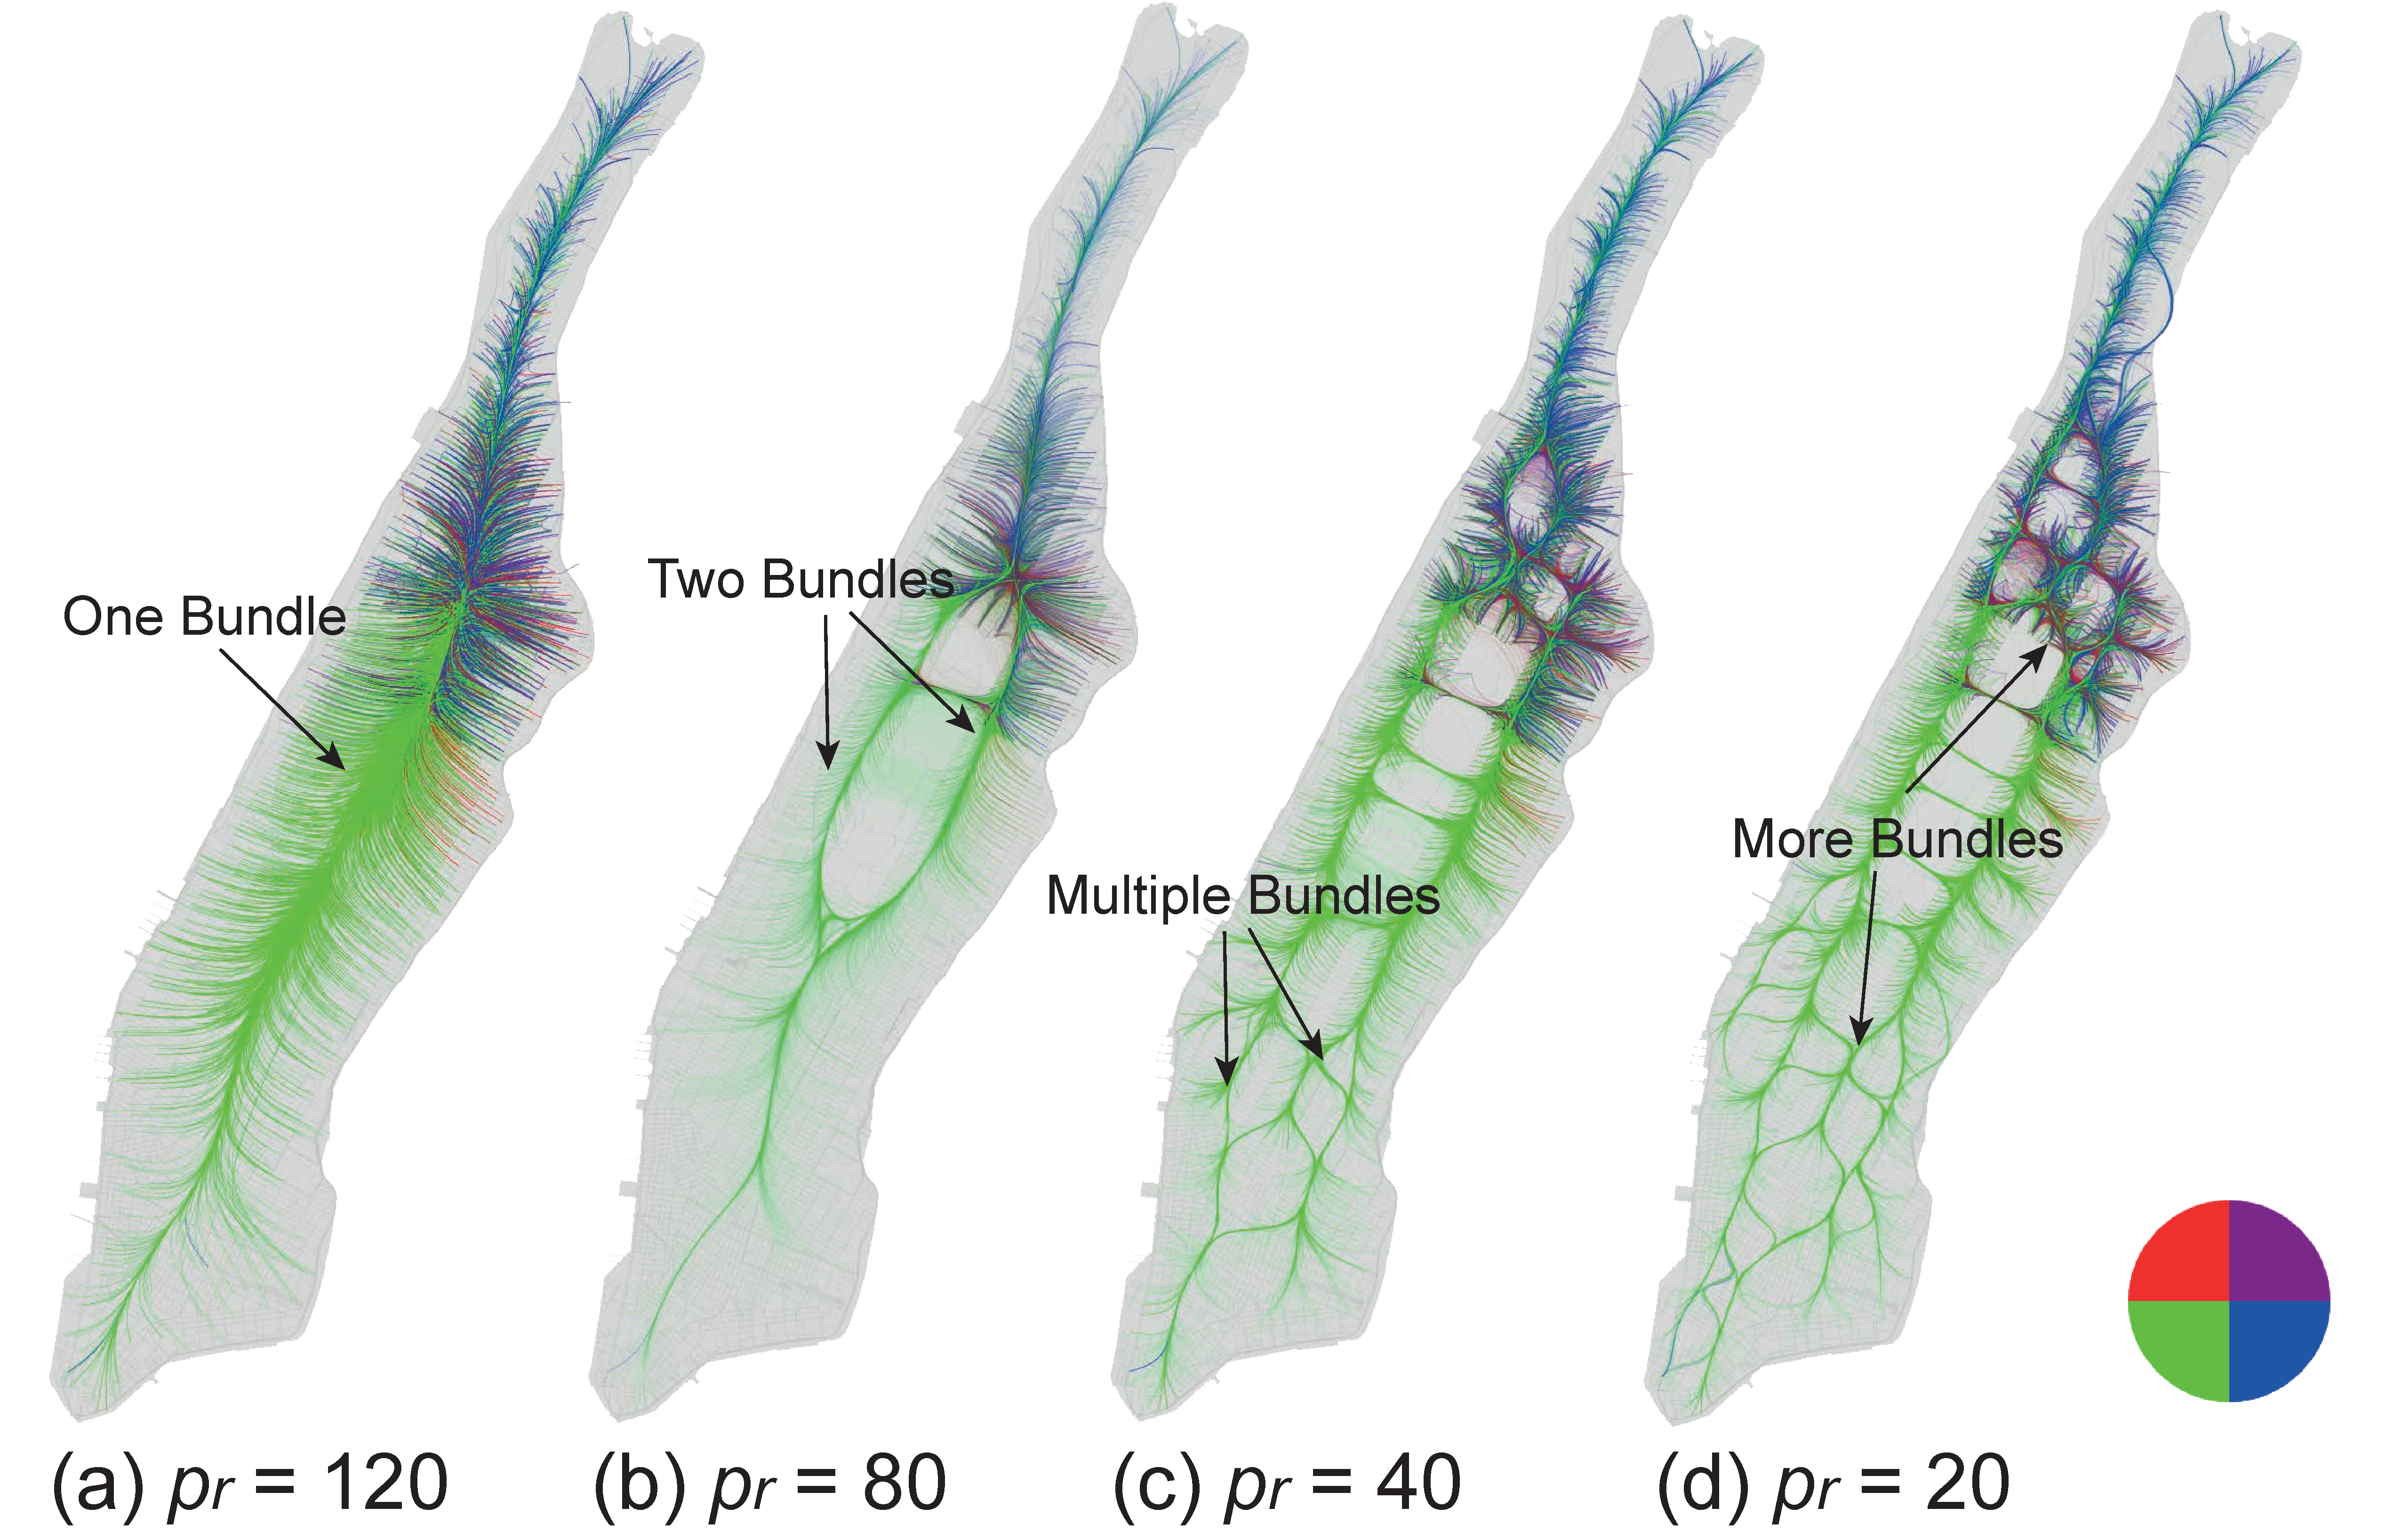
\includegraphics[width=0.495\textwidth]{figure/edgebundling/fig2_kernel_size/kernel_size}
	\vspace{-5mm}
	\caption{KDEEB applied to taxi trips in Manhattan with different kernel sizes $p_r$: (a) 120, (b) 80, (c) 40, and (d) 20.
	More detailed bundles are generated with smaller $p_r$.}
	\label{fig:kernel_size}
	\vspace{-5mm}
\end{figure}

%%%%%%%%%%%%%%%%%%%%%%%%%%%%%%%%%%%%%%%%%%%%%%%%%%%%%%%%%%%%%%%%%%%%
%%%%%%%%%%%%%%%%%%%%%%%%%%%%%%%%%%%%%%%%%%%%%%%%%%%%%%%%%%%%%%%%%%%%

\subsection{KDEEB Algorithm}
\label{ssec:kdeeb}
KDEEB is a fast edge bundling method for visualizing dense graphs.
It employs a general pipeline with edge sampling, splatting, gradient estimation, edge advection, and bundle smoothing.
In edge sampling step, an edge $\textbf{e}_i$ is divided into uniformly-sampled polylines, i.e., $\textbf{e}_i = \{\textbf{x}_j\}$, with user-given sampling step $\sigma$.
After that, KDEEB computes a density map $\rho : \mathbb{R}^2 \rightarrow \mathbb{R}^+ $as

\vspace{-4mm}
\begin{equation}\label{eq:kernel_density_estimation}
\rho(\textbf{x} \in \mathbb{R}^2) = \sum_{\textbf{y} \in D} K (\frac{\|\textbf{x}-\textbf{y}\|}{p_r})
\end{equation}

where $K$ is a parabolic radial kernel and $p_r$ is kernel radius.
Next, each edge sampling site $\textbf{x}_j$ is advected to a new position $\textbf{x}'_j$ as:

\vspace{-5mm}
\begin{equation}\label{eq:advecting_points}
\textbf{x}'_j = \textbf{x}_j + p_r \frac{\nabla \rho}{||\nabla \rho||}
\end{equation}

Finally, a smoothing function is applied on $\textbf{x}_j$ to remove jitters created by the advection step.
These steps are repeated $p_n$ times until stable bundles are generated.

\vspace{2mm}
\noindent
\textit{Parameter Setting}.
KDEEB requires several parameters to be preset by users.
Following settings are recommended~\cite{van2016cubu}:
\begin{itemize}

\item 
Kernel radius $p_r$: Initial value set to 5\% of graph drawing size.
A constant decay ratio $\lambda$ in [0.5, 0.9] is applied to $p_r$ at each bundling iteration $n$.

\item
Bundling iteration $p_n$: An integer in between 10 to 15.

\end{itemize}

\begin{figure*}[t]
	\centering
	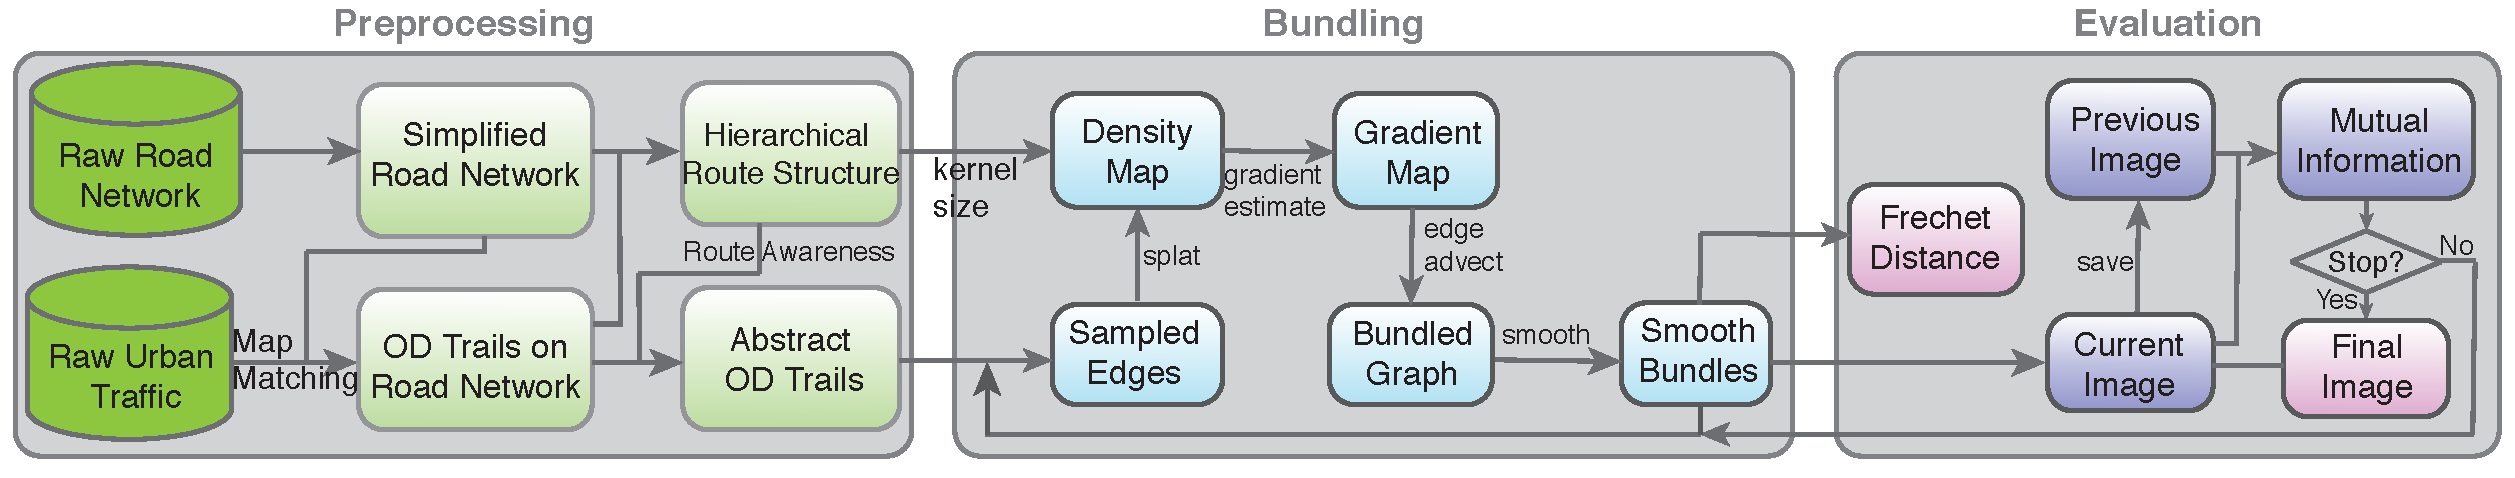
\includegraphics[width=0.995\textwidth]{figure/edgebundling/fig3_framework/framework2.pdf}
	\vspace{-3mm}
	\caption{Overview of RAEB pipeline.
	Our method mainly consists of three phases: \textit{Preprocessing} for creating a proper initial layout, \textit{Bundling} for bundling input OD trails, and \textit{Evaluation} for generating a stable bundle structure.}
	\label{fig:framework}
	\vspace{-4mm}
\end{figure*}

%%%%%%%%%%%%%%%%%%%%%%%%%%%%%%%%%%%%%%%%%%%%%%%%%%%%%%%%%%%%%%%%%%%%
\subsection{Problem Identification}
The parameter settings are recommended for general graphs that consist of fixed nodes and connections between them.
For such a graph, it is free to manipulate node connections into smooth polylines.
However, when applied to OD trails in urban traffic data, KDEEB encounters the following issues.

\begin{itemize}
\item
\textit{P1: Non-optimal Kernel Radius}.
Kernel radius $p_r$ in KDEEB is solely based on graph drawing size, while ignores geometric properties of road network.
Figure~\ref{fig:kernel_size} presents KDEEB results generated with different kernel sizes for taxi trips in Manhattan: 120, 80, 40, and 20 in (a) - (d), respectively.
Sizes for graph drawing are all 720$\times$1440, thus KDEEB would recommend $p_r$ = 80 as 5\% of graph graphing size.
However, smaller $p_r$ generate more detailed and visual appealing bundles, comparing Figure~\ref{fig:kernel_size}(b) to (c) \& (d).
This happens because most space in graph drawing are not utilized, due to the long and thin shape of Manhattan island.
In addition, urban traffic can unevenly spread in a city, such as Shenzhen taxi data (Section~\ref{ssec:study3}), making small $p_r$ preferable.

\vspace{1mm}
\item
\textit{P2: Road Neglect}.
Urban traffic are moving along roads in a city, thus OD trails should be constrained to roads in a city.
However, KDEEB represents each OD connection with a direct line, while ignores information about the road network.
Thus, resulting bundles can be displaced far away from the roads.
This can cause impression of traffic moving in wrong positions, such as those bundles in between Manhattan and Brooklyn (Section~\ref{ssec:study1}).
The displacements can also add difficulty to mentally map original OD trails with resulting bundle lines.
\end{itemize}

\vspace{2mm}
\noindent
Besides, KDEEB lacks a quantitative method to automatically terminate bundling iterations.

\begin{itemize}
\item
\textit{P3: Preset Bundling Iterations}.
KDEEB is an image-based edge bundling method. 
Most of these bundling methods generate bundling results in an iterative way. 
The number of bundling iterations $p_n$ is preset based on practical experience: 10 in KDEEB~\cite{hurter2012graph}, while 15 in CUBu~\cite{van2016cubu}.
The numbers are chosen because tight and stable bundles are generated.
However, these conditions are rather subjective, which can vary among individuals and may be affected by other parameters like image size and sampling step.
\end{itemize}

%%%%%%%%%%%%%%%%%%%%%%%%%%%%%%%%%%%%%%%%%%%%%%%%%%%%%%%%%%%%%%%%%%%%
\subsection{RAEB Overview}
We develop route-aware edge bundling (RAEB), a comprehensive edge bundling method specifically designed for visualizing OD trails in urban traffic.
As illustrated in Figure~\ref{fig:framework}, RAEB pipeline mainly consists of three parts: \textit{Preprocessing}, \textit{Bundling}, and \textit{Evaluation}.

In \textit{Preprocessing}, RAEB first generates a simplified road network from the input one such as open street map (OSM).
Raw OD trails are mapped onto simplified road network using map matching algorithms.
Together with urban traffic information, simplified road network can be organized in a hierarchical route structure.
OD trails can be abstracted accordingly depending on a new parameter of route awareness defined by users.
A value for kernel size is also measured based on geometric property of the route structure.

The abstract OD trails are passed into \textit{Bundling} stage as input graph.
Bundling process is an image-based approach similar to KDEEB workflow.
Specifically, we discard the preset parameter of bundling iteration $p_n$ in KDEEB.
Instead, we introduce a new parameter of bundling stability, which is measured as normalized mutual information between images generated by two consecutive iterations.
The measurement is done in the \textit{Evaluation} stage.
If bundling stability reaches a threshold, we terminate the bundling iteration and export a final image.
Besides, we measure Fréchet distance between generated bundles to OD trails mapped on the road network.
The measurement complements final image with a quantitative metric that reveals quality of a bundling method.

\section{Preprocessing}
\label{sec:preprocess}
%%%%%%%%%%%%%%%%%%%%%%%%%%%%%%%%%%%%%%%%%%%%%%%%%%%%%%%%%%%%%%%%%%%%%%%%%%%%%%%%%%%%%%%%%%%%%%%%%%

This work leverages both OD trails and road network to improve edge bundling quality.
This section introduces major steps in \textit{Preprocessing} stage, including: map matching, hierarchical road structure construction, and trail abstraction.

%%%%%%%%%%%%%%%%%%%%%%%%%%%%%%%%%%%%%%%%%%%%%%%%%%%%%%%%%%%%%%%%%%%%
\subsection{Basic Traffic Concepts}
\textit{Road Network}:
A road network can be modeled as a directed graph $\bar{G} = (\bar{V}, \bar{E})$, where $\bar{V}$ is the set of nodes in $\bar{G}$ and $\bar{E}$ is the set of edges connecting nodes in $\bar{V}$.
Degree of a vertex $\bar{v}$, denoted as $deg(\bar{v})$, indicating the number of edges connected to $\bar{v}$.
By this, a vertex $\bar{v} \in \bar{V}$ can be classified as an endpoint with $deg(\bar{v})=1$, a midpoint with $deg(\bar{v})=2$, or an intersection with $deg(\bar{v})>2$.
To facilitate computation, we can simply $\bar{G}$ into a simplified graph $G = (V, R)$, where $V$ is the union of endpoints and intersections, and $R$ is a set of links connecting nodes in $V$.
Each link $r$ represents a sequence of $n$ consecutive nodes in $\bar{V}$:

\vspace{-7mm}
\begin{equation}
  \begin{aligned}
  	r &:= \bar{v}_1 \rightarrow \bar{v}_2 \rightarrow ... \rightarrow \bar{v}_n, \,\,\, \forall \bar{v}_i \in \bar{V}
  \end{aligned}
\end{equation}

\vspace{-2mm}
\noindent
where $\bar{v}_1$ and $\bar{v}_n$ are endpoints or intersections, while the other nodes are midpoints.
For the sake of clarity, we use the term \textit{route} to describe such a link.
Computation tasks, including shortest path query and map matching, are performed on the simplified graph $G$.

\vspace{1mm}
\noindent
\textit{Urban Traffic}:
Thanks to open data campaign, many urban traffic data are available nowadays.
Typically, raw urban traffic data can come in either of the following forms:

\begin{itemize}
\item
\textit{UT-1}: origin and destination locations only, such as New York taxi trips~\cite{ferreira2013visual} and Singapore public transportation rides~\cite{zeng_2015_visualizing}.
Such a raw trip $t_{raw}$ can be represented as $t_{raw} := l_o \rightarrow l_d$, where $l_o$ and $l_d$ represent origin and destination locations, respectively.

\item
\textit{UT-2}: a sequence of GPS positions, such as Stuttgart scooter fleet~\cite{kruger_trajectorylenses_2013} and Hangzhou taxi trips~\cite{wang_2014_visual-reasoning}.
Such a raw trip $t_{raw}$ can be represented as $t_{raw} := l_1 \rightarrow l_2 \rightarrow ... \rightarrow l_n$, where $l_i \subset \mathbb{R}^2$. $l_1$ and $l_n$ are origin and destination, i.e., $l_o$ and $l_d$.
\end{itemize}

Both forms of urban traffic data can be generalized as a traffic graph $G_t = (L, T)$, where $L$ is the set of locations and $T$ is the set of trips represented as sequential connections of locations.

%%%%%%%%%%%%%%%%%%%%%%%%%%%%%%%%%%%%%%%%%%%%%%%%%%%%%%%%%%%%%%%%%%%%%%%
\subsection{Map Matching}
\label{section:edge_matching}

Constraining movements over an underlying road network, i.e., mapping traffic graph $G_t := (L, T)$ to road network $G := (V, R)$, is usually a preliminary step for urban traffic analysis.
This is necessary.
First, recorded locations get errors due to imprecise GPS localization, while road network is precise and constant.
Second, $G_t$ can be much more complex than $G$:
Taking New York traffic for an example, there are over millions of taxi trips per day, resulting in millions of locations $L$, yet its simplified road network contains less than 100K routes.
Therefore, map matching can enrich effective analysis and visualization.

There are many map matching methods available, including shortest path, minimum turns, and ST-matching~\cite{lou_2009_map} for GPS traces.
These methods are preferable for different dataset.
We employ the following methods for corresponding urban traffic.

\begin{itemize}

\item
For \textit{UT-1}, i.e., $t_{raw} = l_o \rightarrow l_d$, we first find corresponding closest nodes $v_o \in V$, $v_d \in V$ for $l_o$ and $l_d$ respectively.
After that, we search for the shortest path between $v_o$ and $v_d$ in $G$.

\item
For \textit{UT-2}, i.e., $t_{raw} = l_1 \rightarrow l_2 \rightarrow ... \rightarrow l_n$, we use ST-matching algorithm, which considers not only spatial features of road network, but also temporal constraints.
The method was later visually investigated and optimized with an interactive interface~\cite{kruger_2018_visual}.
\end{itemize}

Both methods return a sequence of routes $r_1 \rightarrow r_2 \rightarrow ... \rightarrow r_n$ in $G$ for each OD trail $t_{raw}$.
We then combine the routes with origin ($l_o$) and destination ($l_d$) locations of $t_{raw}$.
Thus, both types of $t_{raw}$ are converted to the same map matching form. 

\vspace{-7mm}
\begin{equation}
  	\begin{aligned}
t_{map} := l_o \rightarrow r_1 \rightarrow r_2 \rightarrow ... \rightarrow r_n \rightarrow l_d.
 	\end{aligned}
\end{equation}
\vspace{-1mm}

Here the OD trail's origin $l_o$ and destination $l_d$ are kept.

%%%%%%%%%%%%%%%%%%%%%%%%%%%%%%%%%%%%%%%%%%%%%%%%%%%%%%%%%%%%%%%%%%%%%%%%%%%%%%%%%%%%%%%%%%%%%%%%%%
\subsection{Hierarchical Route Structure Construction}
\label{ssec:hiera_road}

\begin{table}
	\centering
	\begin{tabular}{|c|c|c|}
	\hline
	Category & Exemplary OSM Indicator & Score ($r_{hier}$)  \\ \hline
	Expressway & motorway, trunk & 1 \\ \hline
	Trunk Road & primary, motorway\_link& 0.75 \\ \hline
	Secondary Road & secondary, tertiary & 0.5 \\ \hline
	Branch Road & unclassified, residential & 0.25 \\ \hline
	\end{tabular}
	\vspace{1mm}
	\caption{Route hierarchy, OSM indicator and hierarchy score} \label{tab:sometab}
	\label{table: road_score}
\vspace{-6mm}
\end{table}

A road network is usually designed in hierarchical levels to avoid dense direct connections among regions.
This inspires us to construct a hierarchical route structure to benefit edge bundling.
Although urban roads are organized hierarchically, it does not consider OD trails.
This work makes use of the following attributes of a route $r$ in $G := (V, R)$ to construct a hierarchical route structure.

\vspace{1mm}
\noindent
\textit{Route length} ($len(r)$).
Visual appearance of each OD trail is determined by its routes on road network.
Longer a route, more it will affect the visual appearance.
Thus an important component affecting route hierarchy is route length.
Here, $len(r)$ is measured in Euclidean space and normalized over the whole road network.

\vspace{1mm}
\noindent
\textit{Road hierarchy} ($hier(r)$).
Urban roads are classified into hierarchies: freeways, arterials, collectors, and local roads.
Similar descriptions can also be found elsewhere~\cite{wang_2014_visual-reasoning}.
A higher level usually indicates faster traffic speed and less access to property.
OSM provides more detailed indicators of road hierarchy, e.g., trunk, primary, tertiary, etc.
To keep consistent, we classify these indicators into four hierarchies.
A route $r$ in each hierarchy is assigned an score according to Table~\ref{table: road_score}. 

\vspace{1mm}
\noindent
\textit{Flow magnitude} ($flow(r)$).
Flow magnitude measures how many OD trails pass through a route $r$.
The previous two factors purely rely on road network, while $flow(r)$ reflects the importance of a route in consideration of OD trails.
Here, $flow(r)$ is measured by counting how many mapped OD trails passing through $r$, and then normalized. 

\vspace{2mm}
By this, each route can be represented by a vector $V(r) := <len(r), hier(r), flow(r)>$.
Score of a route $score(r)$ can be measured as $score(r) = \sum w_i \times V(r)_i$, where the weights $w_i (i = 1, 2, 3)$ controls how much each attribute affects route weight.
We choose 0.3, 0.1, and 0.6 in this work, which highlights the importance of flow magnitude.
In the end, all routes are sorted in descending order according to their weights.
The routes $R$ are further subdivided into multiple hierarchical levels $R^1$, $R^2$, ..., $R^n$.
Each level of routes accounts for top-k routes.

\begin{figure}[t]
	\centering
	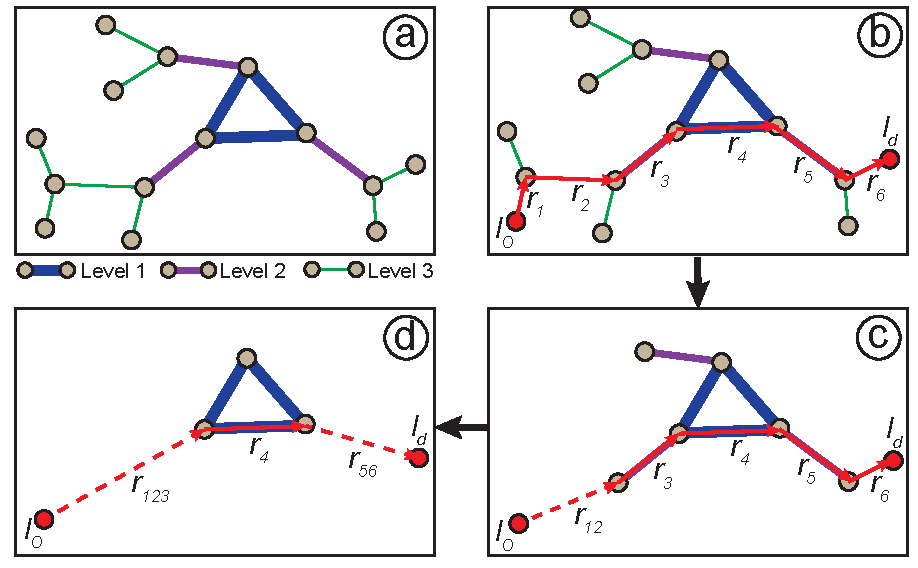
\includegraphics[width=0.7\textwidth]{figure/edgebundling/fig4_od_abstraction/OD_Abstraction.pdf}
	\vspace{-3mm}
	\caption{Illustration of hierarchical route structure and OD trail abstraction:
	(a) Three route levels are constructed colored in blue, purple and green, repsectively; a raw OD trail is abstracted in accordance to route (b) level-3, (c) level-2, and (d) level-1.}
	\label{fig:road_hierarchy}
	\vspace{-1mm}
\end{figure}

%%%%%%%%%%%%%%%%%%%%%%%%%%%%%%%%%%%%%%%%%%%%%%%%%%%%%%%%%%%%%%%%%%%%%%%%%%%%%%%%%%%%%%%%%%%%%%%%%%
\subsection{Trail Abstraction}
\label{section: trail_abstraction}

\textbf{P2} states that road network is omitted in original KDEEB, which can lead to wrong depiction in geographical space and poor support of multi-scale exploration.
We introduce a new parameter of route awareness $p_{ra}$, which defines the level of trail abstraction, to tackle this issue.
Higher $p_{ra}$ indicates that more details of OD trails should be preserved.
Given a hierarchical route structure in $n$ levels, $p_{ra}$ can range from 0 to $n$.
If $p_{ra}$ is set to zero, OD trails will be abstracted to straight lines connecting ODs directly.
If $p_{ra}$ is set to $n$, no abstraction will be applied.
If $p_{ra}$ is set to a value $m$ in [1, $n-1$], routes in level-1 to level-$m$ will be preserved.

Figure~\ref{fig:road_hierarchy}(a) presents an exemplary road network with a hierarchical route structure.
The routes are categorized into three levels: blue thick lines for level 1, purple medium lines for level 2, and green thin lines for level 3.
Figure~\ref{fig:road_hierarchy}(b-d) illustrates an example of how a raw OD trail of $l_o \rightarrow r_1 
\rightarrow...\rightarrow r_6 \rightarrow l_d$ can be abstracted in accordance to the hierarchical route structure shown in Figure~\ref{fig:road_hierarchy}(a).
In Figure~\ref{fig:road_hierarchy}(b), $p_{ra}$ is set 3, and all routes are preserved.
In Figure~\ref{fig:road_hierarchy}(c), $p_{ra}$ is set 2, so route $r_1$ and $r_2$ will be merged together as they are both level-3 routes.
In Figure~\ref{fig:road_hierarchy}(d), $p_{ra}$ is set 1, thus only route $r_4$ will be kept.
\section{Bundling Method}
\label{sec:bundling}

RAEB adapts KDEEB bundling algorithm~\cite{hurter2012graph} to better reveal topology of urban traffic.
This sections presents amendments employed by RAEB, including kernel size measurement and density map generation.

\begin{algorithm}[b]
	\caption{KernelSizeMeasurement}\label{al:kernel_size_measurement}
	\begin{algorithmic}[1]
		\Require Top \textit{N} sorted routes as polyline list $\textbf{P} = \{P_1, ..., P_N\}$
		\Ensure Initial kernel size $p_r$		
		\State Let $d$[ ][ ] denote distance between polyline pairs
		\For {i = 1 to $N$}
			\For {j = i + 1 to $N$}
			\State $d$[i][j] = $d$[j][i] = DiscreteFrechetDistance($P_i$, $P_j$)
			\EndFor
		\EndFor
		\State Let \textbf{C} denote a list of polyline clusters;
		\State \textbf{C} = $DBSCAN(\textbf{P}, eps, minNum)$;
		\State $C_{max}$ = $argmax_{|C_i|}(C_i | C_i \in \textbf{C})$;
		\State Initialize $d_{geo} = 0$;
		\State Let $count = |C_{max}| \times (|C_{max}| - 1)$;
		\ForEach {$P_i \in C_{max}$}
			\ForEach {$P_j \in C_{max}$ \&\& $P_i \neq P_j$}
				\State $d_{geo}$ = $d_{geo}$ + $d$[i][j] / count;
			\EndFor
		\EndFor
		\State $p_r$ = ToDrawingSpace($d_{geo}$ / 2); \\
		\Return $p_r$
	\end{algorithmic}
\end{algorithm}

%%%%%%%%%%%%%%%%%%%%%%%%%%%%%%%%%%%%%%%%%%%%%%%%%%%%%%%%%%%%%%%%%%%%%%%%%%%%%%%%%%%%%%%%%%%%%%%%%%
%%%%%%%%%%%%%%%%%%%%%%%%%%%%%%%%%%%%%%%%%%%%%%%%%%%%%%%%%%%%%%%%%%%%%%%%%%%%%%%%%%%%%%%%%%%%%%%%%%
\subsection{Optimal Kernel Size}
\label{ssec:kernel_size}
KDEEB only considers the size of graph drawing when determining kernel size.
This strategy may not be optimal for bundling OD trails in urban traffic (\textit{P1}).
Ideally, the chosen kernel size should be able to bundle closely-related OD trails (e.g., movements on bi-directional roads), while separate loosely-correlated OD trails (e.g., movements on two different highways).

To address \textit{P1}, both graph drawing size and geometric property of road network should be considered.
We develop an automatic process for measuring initial kernel size, as outlined in Algorithm~\ref{al:kernel_size_measurement}.
Here, top $N$ routes are extracted from \textit{Preprocessing} stage.
The routes are treated as a polyline list \textbf{P}, and inputted into the algorithm.
Pair-wise distance between each pair of ploylines are computed. 
Then a DBSCAN algorithm is applied to group the polylines into polyline clusters \textbf{C}.
The cluster with maximum number of polylines is extracted, and denoted as $C_{max}$.
Average geographical distance $d_{geo}$ is computed for polylines in $C_{max}$.
Finally, half of $dist_{geo}$ is converted to $p_r$ in graph drawing space, and $p_r$ is returned as the initial kernel size.

Basically, the algorithm first computes average geographical route distance in the top $N$ routes, and then converts the distance to graph drawing space.
$N$ should not be too small that the routes are not representative for the whole road network; meanwhile, it should not be too big to overlap route awareness.
From our experiments, we find 1\% of whole route size is appropriate for $N$.
Besides, another important factor is the distance metric between two polylines.
Here, we choose discrete Frechet distance, which measures similarity of two polylines considering both locations and ordering of the points along the polylines.
The metric is one of the most popular methods for movement analysis~\cite{gudmundsson2011computational}, and can be computed efficiently~\cite{eiter_1994_computing}.

%%%%%%%%%%%%%%%%%%%%%%%%%%%%%%%%%%%%%%%%%%%%%%%%%%%%%%%%%%%%%%%%%%%%%%%%%%%%%%%%%%%%%%%%%%%%%%%%%%
%%%%%%%%%%%%%%%%%%%%%%%%%%%%%%%%%%%%%%%%%%%%%%%%%%%%%%%%%%%%%%%%%%%%%%%%%%%%%%%%%%%%%%%%%%%%%%%%%%
\subsection{Density Map Generation}
KDEEB omits trail information (\textit{P3}), as it connects ODs with directed lines.
We aim to keep bundles close to OD trails on road network.
More specifically, in \textit{Preprocessing} stage, each OD trail is abstracted into a sequence of artificial directed lines and real routes in road network.
The artificial directed lines are free to manipulated, while we would like to keep the bundle layout spatially close to the real routes.
In addition, it is preferable to keep the bundling paradigm of advecting sampling sites towards high density directions.

To achieve this goal, we modify the density map generation used by KDEEB.
Let denote a list of routes $R_{aware} \subset \mathbb{R}^2$ are kept for route awareness.
Since sampling sites are advected towards their gradient directions, gradients of points along $R_{aware}$ should be either (1) zero, or (2) pointing to route direction.
To minimize effects on densities surrounding $R_{aware}$, we choose the second option.
Instead of Eqn.~\ref{eq:kernel_density_estimation}, we now use

\vspace{-5mm}
\begin{equation}\label{eq:new_density}
\rho_{od} = \rho + D(\textbf{x} | \textbf{x} \in R_{aware})
\end{equation}
\vspace{-3mm}

\noindent
where $D(\textbf{x}) \in \mathbb{R}^+$ is a constant assigned to a point $\textbf{x} \in R_{aware}$.
High $D$ value will make it more likely that gradient at $\textbf{x}$ points to the same direction with the route.

\section{Evaluation}
\label{sec:eva}

Besides introduction of \textit{Preprocessing} and adaptions in \textit{Bundling}, post hoc bundling evaluation methods are also developed in RAEB.
This section introduces these methods, including mutual information and bundle deviation measurements.

%%%%%%%%%%%%%%%%%%%%%%%%%%%%%%%%%%%%%%%%%%%%%%%%%%%%%%%%%%%%%%%%%%%%%%%%%%%%%%%%%%%%%%%%%%%%%%%%%%
\subsection{Normalized Mutual Information}
After each bundling iteration, a bundling method needs to decide whether the bundling iteration should continue or not.
KDEEB presets a bundling iteration parameter $p_n$, similar to many other bundling methods including SBEB, FTTEB, and CUBu.
$p_n$ = 10 is chosen such that the bundles converge to a stable structure.
Structure stability is basically the perception of visual similarity between images generated in two consecutive bundling iterations.
However, the perception can be easily biased by many factors, including people's color perception difference, lighting conditions, etc.
It lacks a quantitative method for measuring structure stability.

\begin{figure}[t]
	\centering
	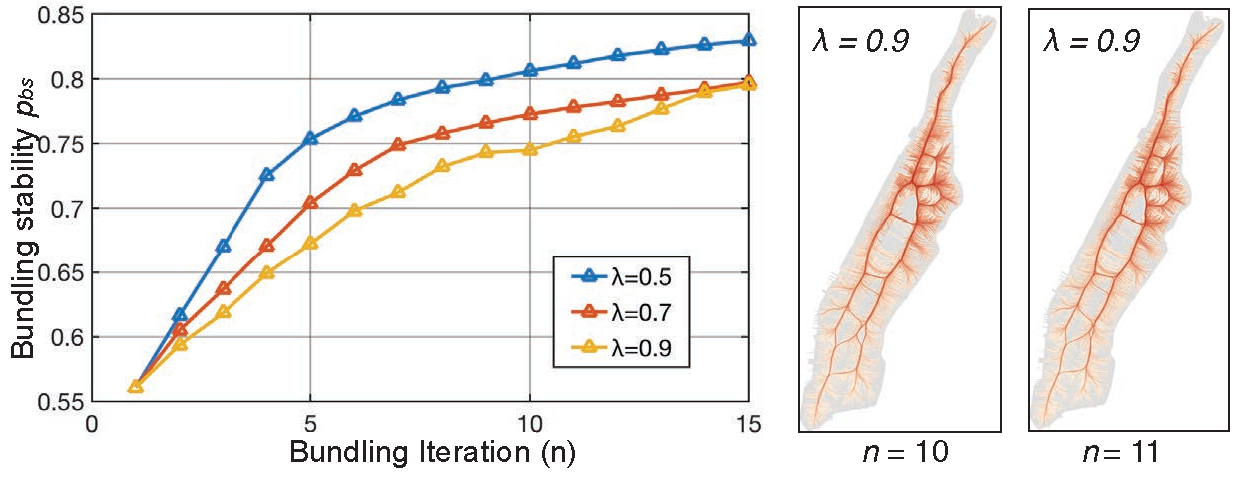
\includegraphics[width=0.7\textwidth]{figure/edgebundling/fig5_NMI/bundle_termination.pdf}
	\vspace{-5mm}
	\caption{(left) Bundling stability $p_{bs}$ measured at each bundling iteration for different decay ratios $\lambda$, (right) visually indistinguishable images are generated at iteration 10 and 11 for $\lambda=0.9$.}
	\label{fig:nmi}
	\vspace{-1mm}
\end{figure}

%%%%%%%%%%%%%%%%%%%%%%%%%%%%%%%%%%%%%%%%%%%%%%%%%%%%%%%%%%%%%%%%%%%%%%%%%%%%%%%%%%%%%%%%%%%%%%%%%%

%%%%%%%%%%%%%%%%%%%%%%%%%%%%%%%%%%%%%%%%%%%%%%%%%%%%%%%%%%%%%%%%%%%%%%%%%%%%%%%%%%%%%%%%%%%%%%%%%%

We employ mutual information (MI) - a basic concept from information theory, as a quantitative indicator for measuring bundling stability.
Maes et al.~\cite{maes1997multimodality} introduced MI to measure statistic dependence between intensities of corresponding voxels in two medical images.
This work measures MI between images generated in consecutive bundling iterations, which are geometrically aligned.
Hence, the measurement is simplified without geometry matching. 
Let denote two input images $X$ and $Y$.
MI is computed as:

\vspace{-6mm} 
\begin{equation} \label{eq:mi}
I(X, Y) = \sum_{x}\sum_{y}p(x,y)log(\frac{p(x,y)}{p(x)p(y)}))
\end{equation}

\noindent
where $p(x)$ and $p(y)$ indicate the intensity at $x \in X$ and $y \in Y$, and $p(x, y)$ measures the joint value between $p(x)$ and $p(y)$.
MI is affected by image size, while we prefer a constant measurement for different graph drawings.
Hence, we adopt normalized MI (NMI):

\vspace{-6mm} 
\begin{equation}\label{eq:nmi}
NMI(X, Y) = \frac{2I(X,Y)}{H(X) + H(Y)} 
\end{equation}

\noindent
where $H(X) = -\sum p(x)log(p(x)))$ that measures entropy for $X$.

We introduce a new parameter of bundling stability $p_{bs}$.
$p_{bs}$ is computed in every iteration as NMI($I_n$, $I_{n-1}$), where $I_n$ and $I_{n-1}$ denote images generated at iteration $n$ and $n-1$, respectively.
Figure~\ref{fig:nmi}(left) presents NMIs at each bundling iteration for three different kernel size decay ratios $\lambda$.
It is observed that NMI increases when bundling iteration increases, and smaller $\lambda$ leads to faster NMI increment.
All NMIs pass over 0.75 around iteration 10, and reach close to 0.8 at iteration 15.
Figure~\ref{fig:nmi}(right) shows two images at iteration 10 and 11 for $\lambda$ = 0.9.
The images are hardly distinguishable from each other.
Thus, we can claim the bundling produces stable results, and the process can terminate.
In this way, we determine a threshold for $p_{bs}$ to control bundle termination.
If a bigger threshold is chosen, more stable results will be generated.

%%%%%%%%%%%%%%%%%%%%%%%%%%%%%%%%%%%%%%%%%%%%%%%%%%%%%%%%%%%%%%%%%%%%%%%%%%%%%%%%%%%%%%%%%%%%%%%%%%
\subsection{Bundle Deviation}
$p_{bs}$ is introduced for measuring visual stability of bundle layouts generated by one bundling method.
However, $p_{bs}$ is not suitable for comparing bundling quality of multiple bundling methods.
Many evaluation metrics can be used for comparing graph layouts, such as edge crossing, ambiguity, and edge direction.
These metrics are suitable for general graphs without a ground truth.
However, OD trails studied in this work are constrained in roads in a city.
We would like to keep the generated bundles close to their OD trails on the road network.
Though map matching algorithm can intrdouces errors, this work treats mapped OD trails as ground truth, instead of raw OD trails.
This is because of: for \textit{UT-1} urban traffic, only origin and destination information are recorded; for \textit{UT-2} urban traffic, accuracy of GPS positions are not perfect.

We introduce a new parameter of bundle deviation, denoted as $p_{d}$, to measure distance between final bundles and OD trails mapped on the road network.
Both bundles and OD trails can be modeled as polylines made up of sequential positions in geographical space.
Thus, the distance between them can be measured using discrete Frechet Distance.
We calculate mean distances for all bundles, and map the mean in graph drawing space.
\begin{figure}[t]
	\centering
	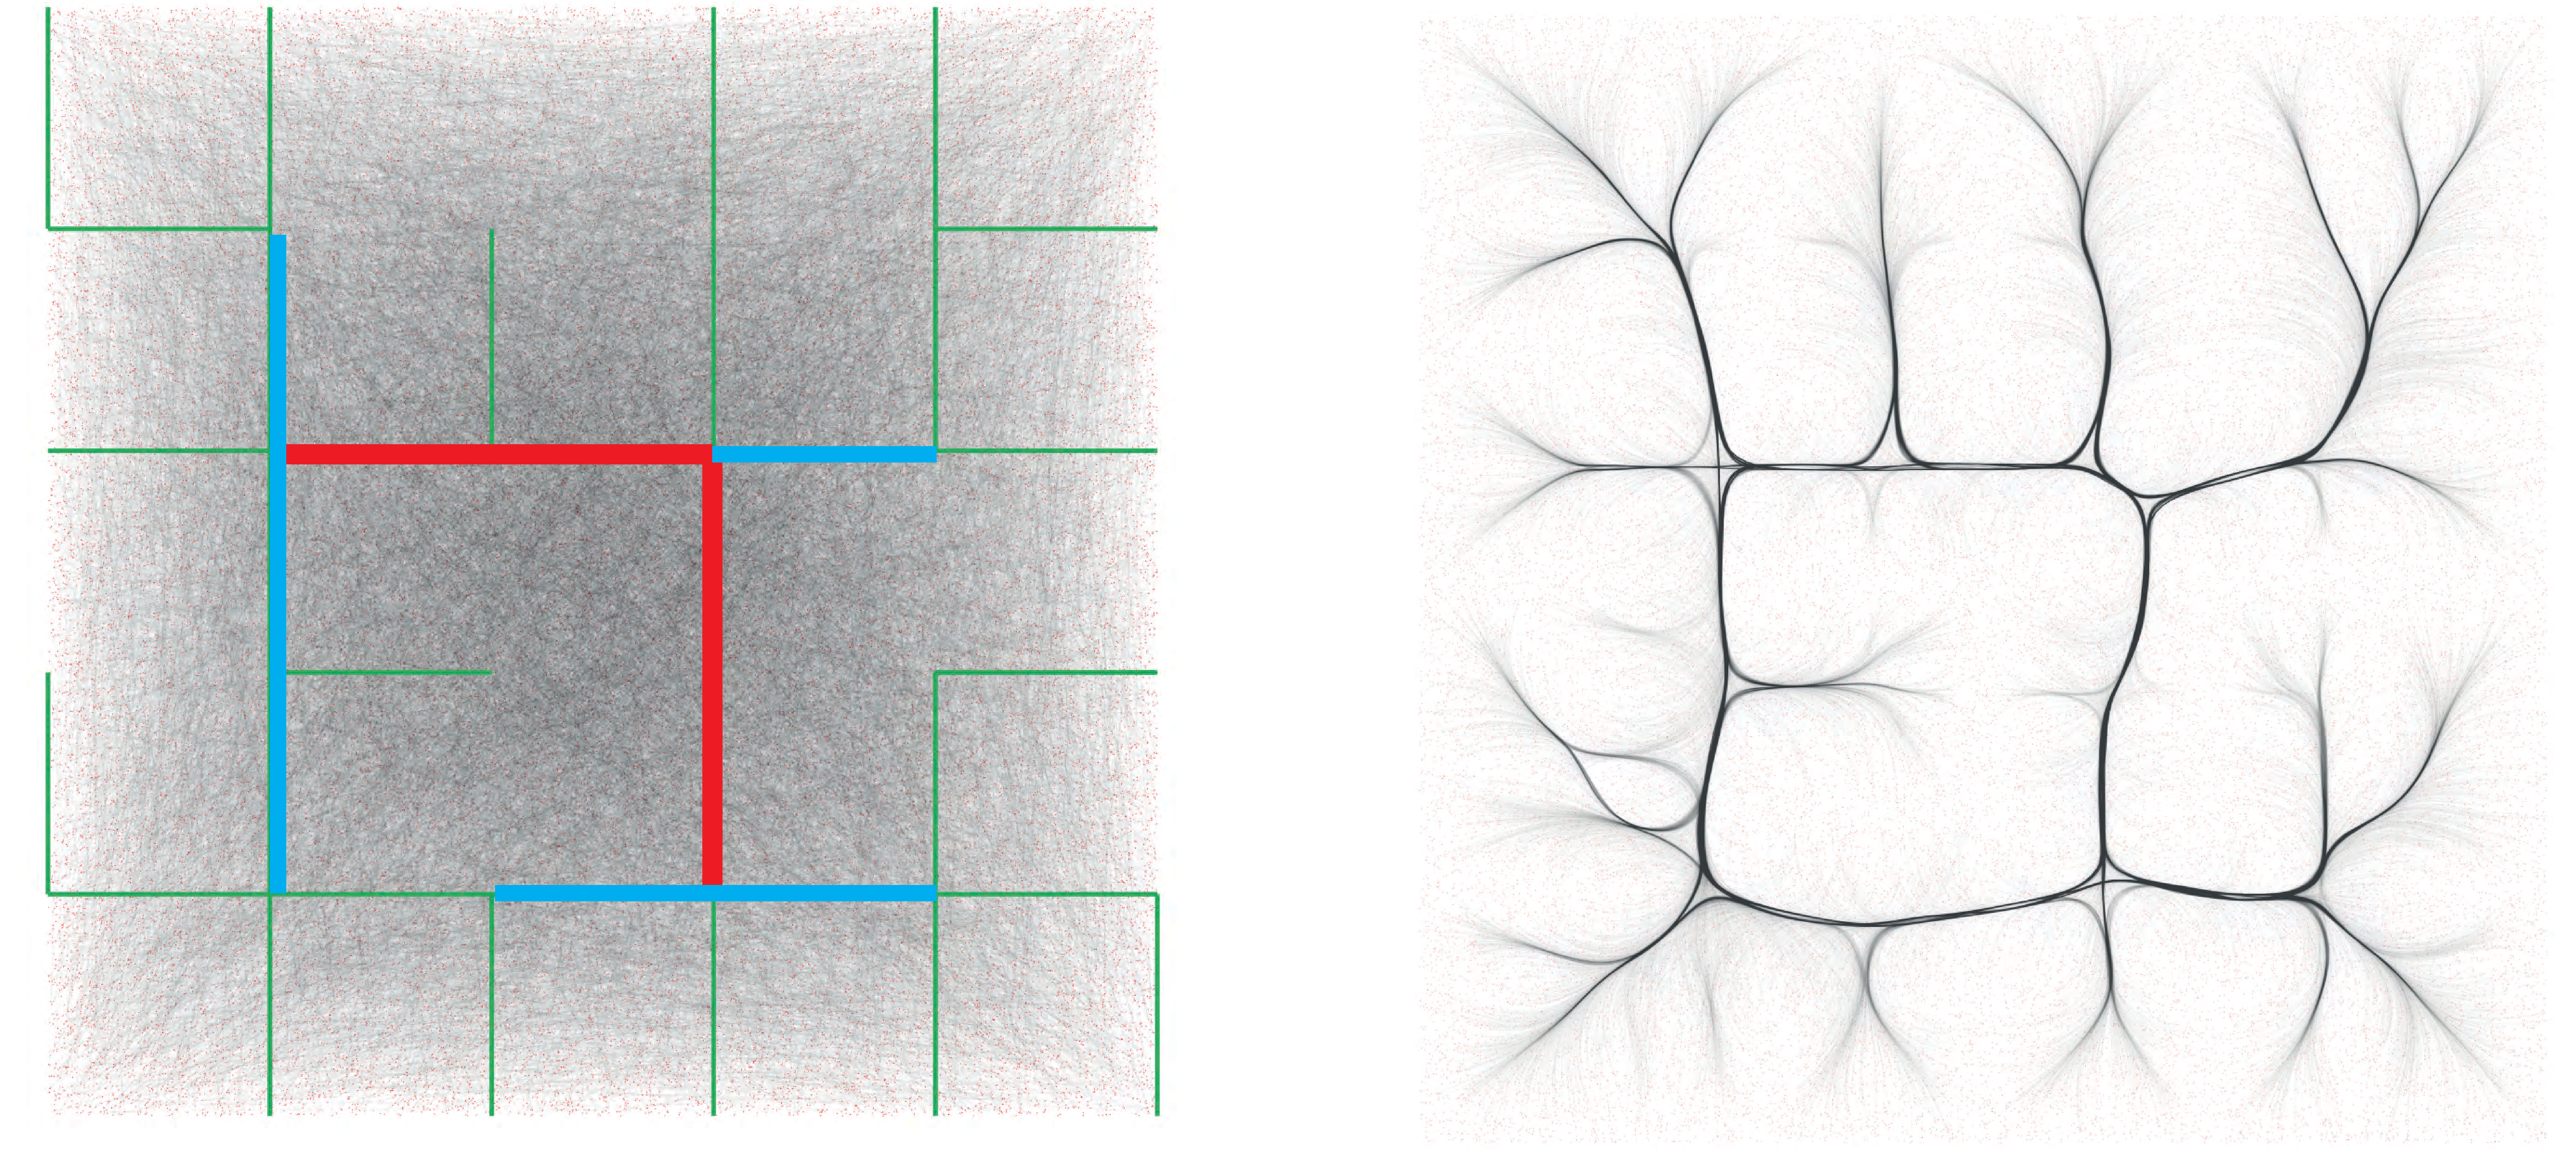
\includegraphics[width=0.49\textwidth]{fig7_hierar/artifical}
	\vspace{-6mm}
	\caption{
		Left: raw 100K artificial OD trails on a hierarchical road network.
		Right: RAEB bundling result with $p_{ra}$ set to 2.
		}
	\label{fig:hier}
	\vspace{-5mm}
\end{figure}

\section{Applications}
This section presents applications of RAEB on artificial OD trails, and real-world taxi data in New York and Shenzhen.
We show advancements of RAEB over KDEEB.

\begin{figure*}[t]
	\centering
	\includegraphics[width=0.995\textwidth]{fig8_study2/NYC}
	\vspace{-2mm}
	\caption{Density maps of NYC taxi trips:
	(a) shortest paths mapped onto the road network, 
	(b) KDEEB bundles with kernel size $p_r$ = 60,
	(c) KDEEB bundles with $p_r$ = 21,
	and (d) our RAEB bundles with $p_r$ = 21.}
	\label{fig:nyc_visual}
	\vspace{-4mm}
\end{figure*}

\begin{figure}[t]
	\centering
	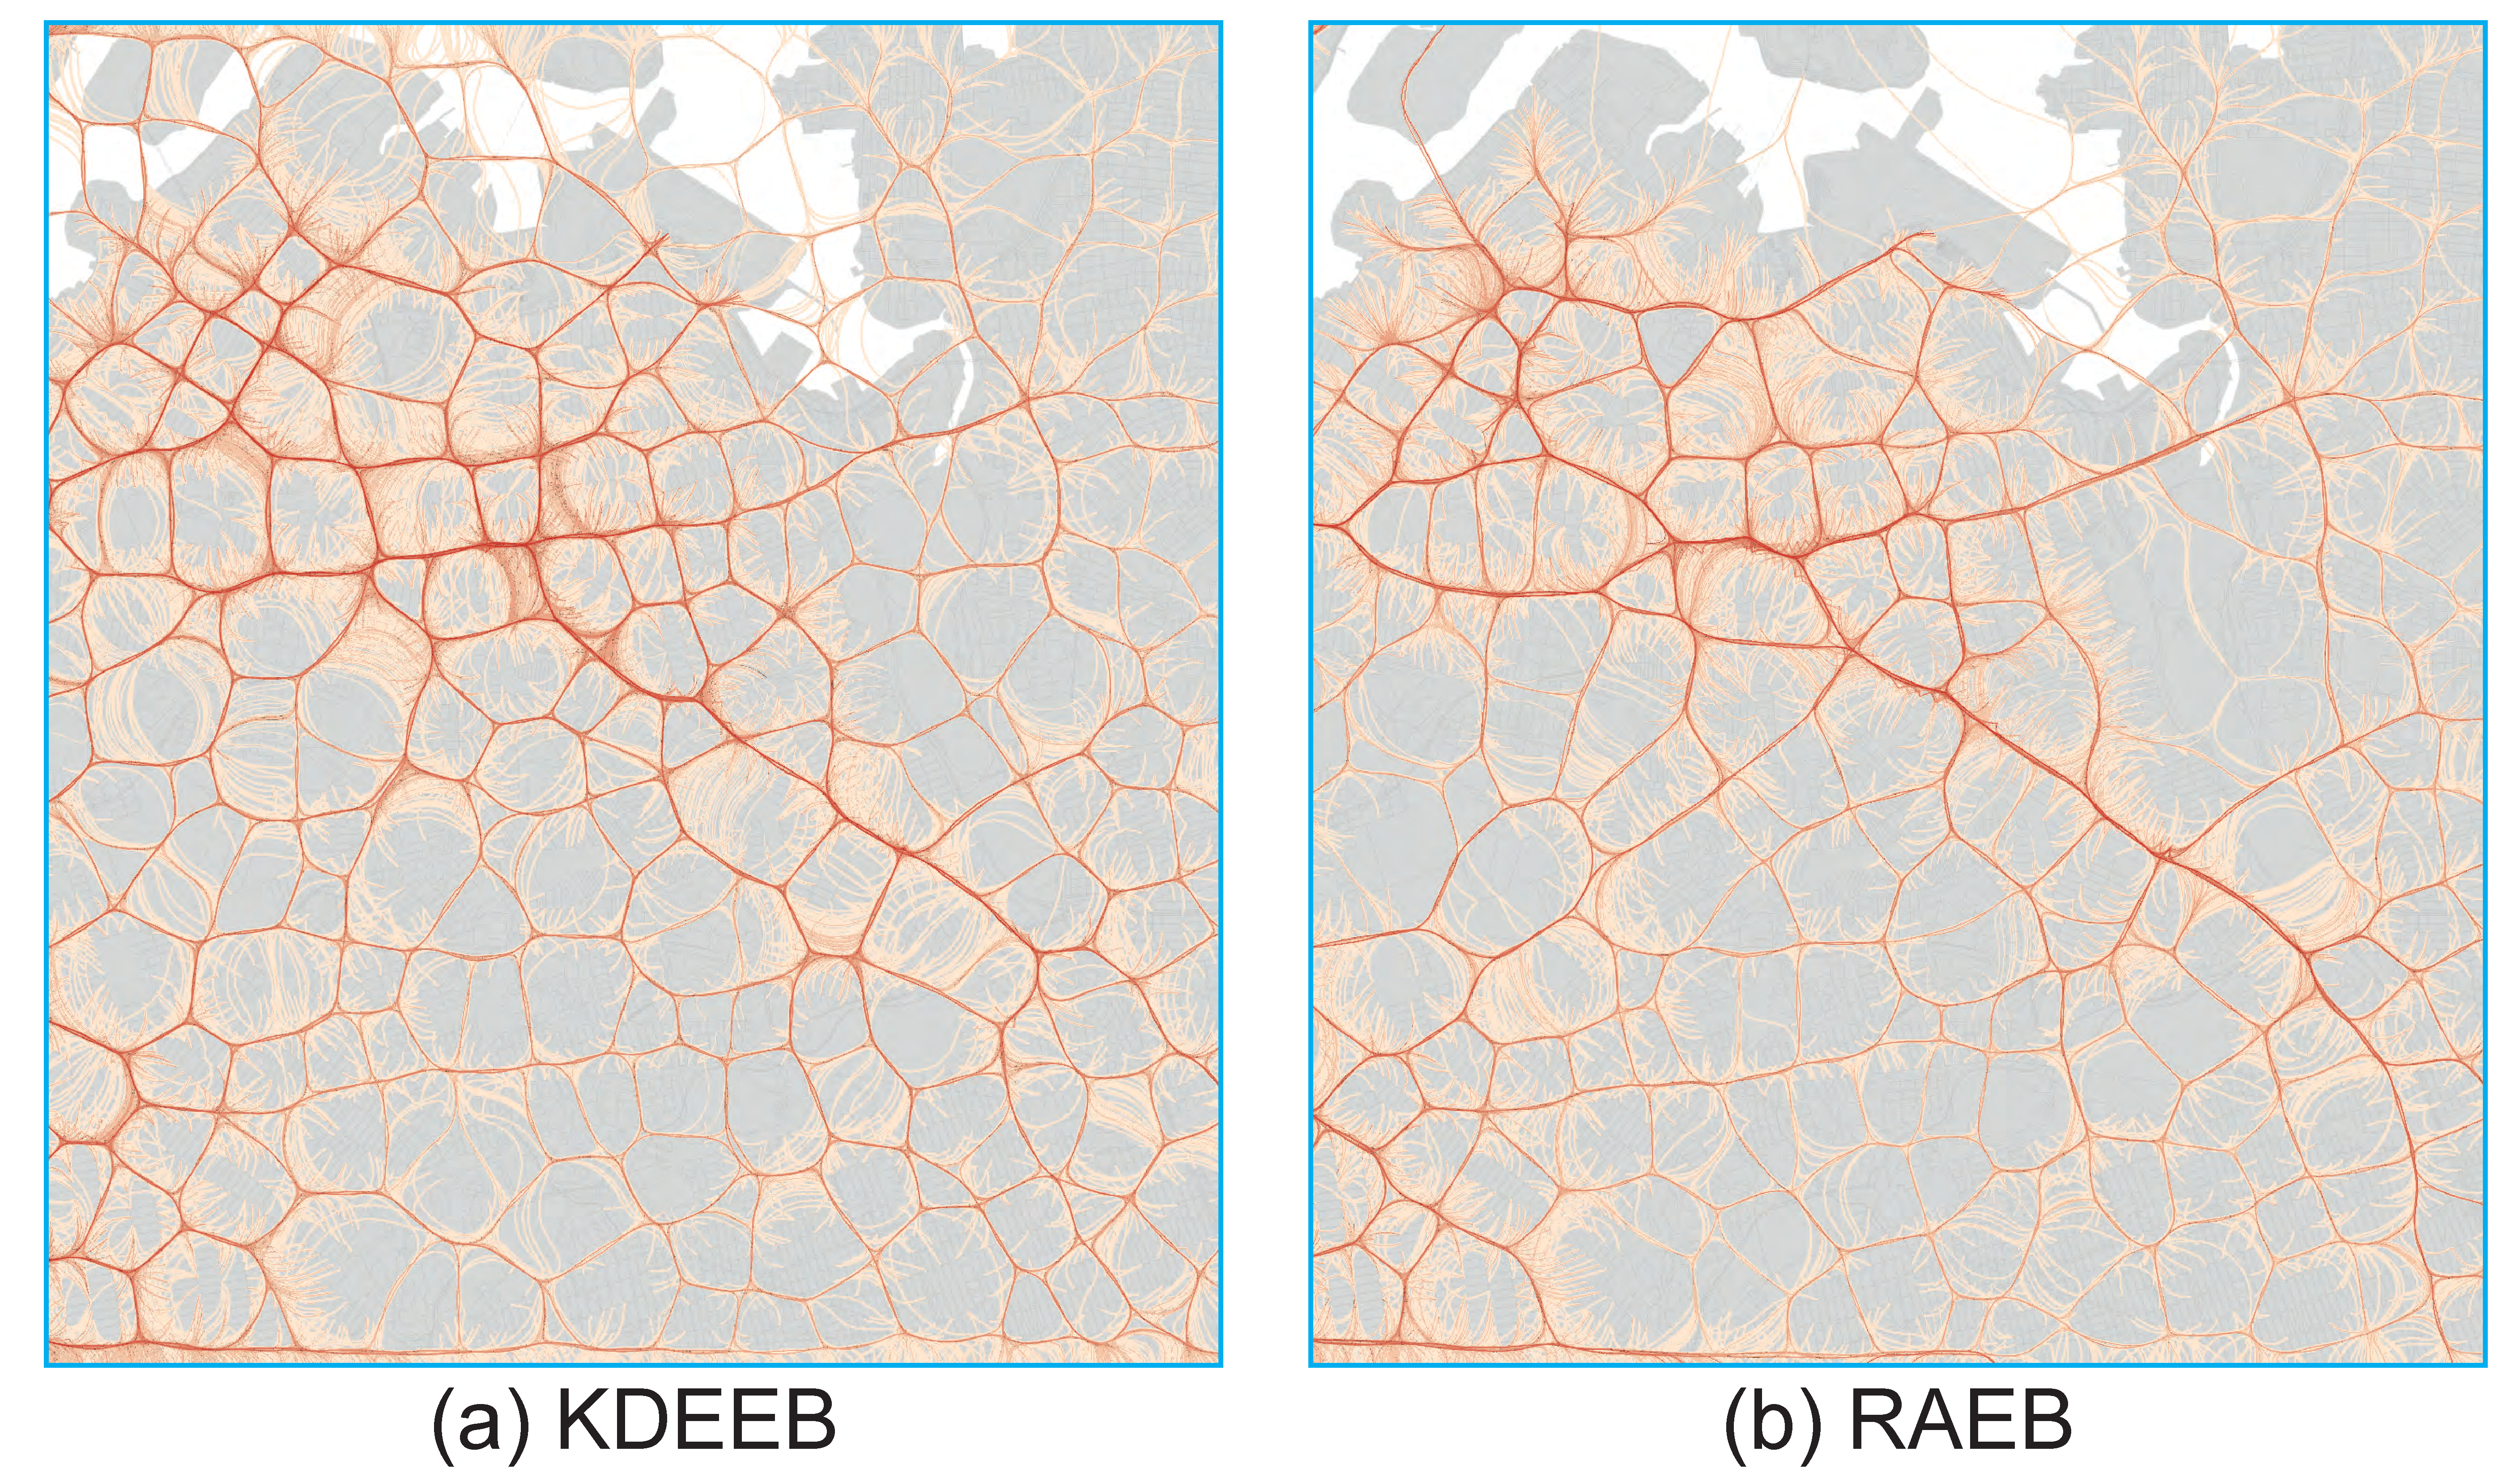
\includegraphics[width=0.45\textwidth]{fig9_study2-2/NYC-zoom}
	\vspace{-3mm}
	\caption{Fine scale density maps of NYC taxi trips in Queens zone generated by (a) KDEEB, and (b) RAEB.}
	\label{fig:nyc-zoom}
	\vspace{-4mm}
\end{figure}

%%%%%%%%%%%%%%%%%%%%%%%%%%%%%%%%%%%%%%%%%%%%%%%%%%%%%%%%%%%%%%%%%%%%%%%%%%%%%%%%%%%%
\subsection{Artificial OD Trails}
\label{ssec:study1}

Our first example uses a random graph with 100K OD trails, and $5 \times 5$ grid and hierarchical reference graphs to simulate conventional road networks.
Raw OD trials and corresponding road networks are shown in the leftmost figures of Figure~\ref{fig:grid} and Figure~\ref{fig:hier}.
The OD trails are first mapped to underlying road networks using shortest path algorithm, and then both road networks are divided into three hierarchies that are colored in red, blue and green, receptively.
In the last, we apply RAEB on the OD trails, with all graph drawing sizes set to 1280$\times$1280 and initial kernel sizes $p_r$ set to 60.

In advance of KDEEB, RAEB allows to preserve route awareness by controlling parameter $p_{ra}$.
To evaluate the effects of $p_{ra}$, we set $p_{ra}$ to 0 - 3, and apply RAEB to OD trails on the grid road network as shown in the leftmost figure of Figure~\ref{fig:grid}.
The results are shown in Figure~\ref{fig:grid} (a) - (d).
In (a), $p_{ra}$ is set to 0, i.e., no route awareness will be preserved.
In this case, RAEB should be equivalent to KDEEB with other parameters the same.
The proof is demonstrated in (a), which shows smooth bundles similar to those in the original KDEEB~\cite{hurter2012graph}.
To preserve level 1 routes, we set $p_{ra}$ to 1, and the result is shown in (b).
As expected, OD trails around the red lines are bundled together with bundles following red lines, while other OD trails are bundled with bundles spreading arbitrarily in the graph drawing.
More route awareness can be preserved as we increase $p_{ra}$ to 2 and 3, as shown in Figure~\ref{fig:grid} (c) \& (d).

More importantly, route awareness $p_{ra}$ can be used to preserve topology of underlying road network.
Figure~\ref{fig:hier} (right) shows bundling result of RAEB applied to OD trails on a hierarchical road network that is shown in Figure~\ref{fig:hier}(left).
Here, $p_{ra}$ is set to 2, such that to preserve both the red and blue lines.
It is clear that the resulting bundles follow the lines, making it easy to trace OD trails.
In contrast, KDEEB will generate the same result with that in Figure~\ref{fig:grid}(a), as the underlying road network information is not used.

\begin{figure*}[t]
	\centering
	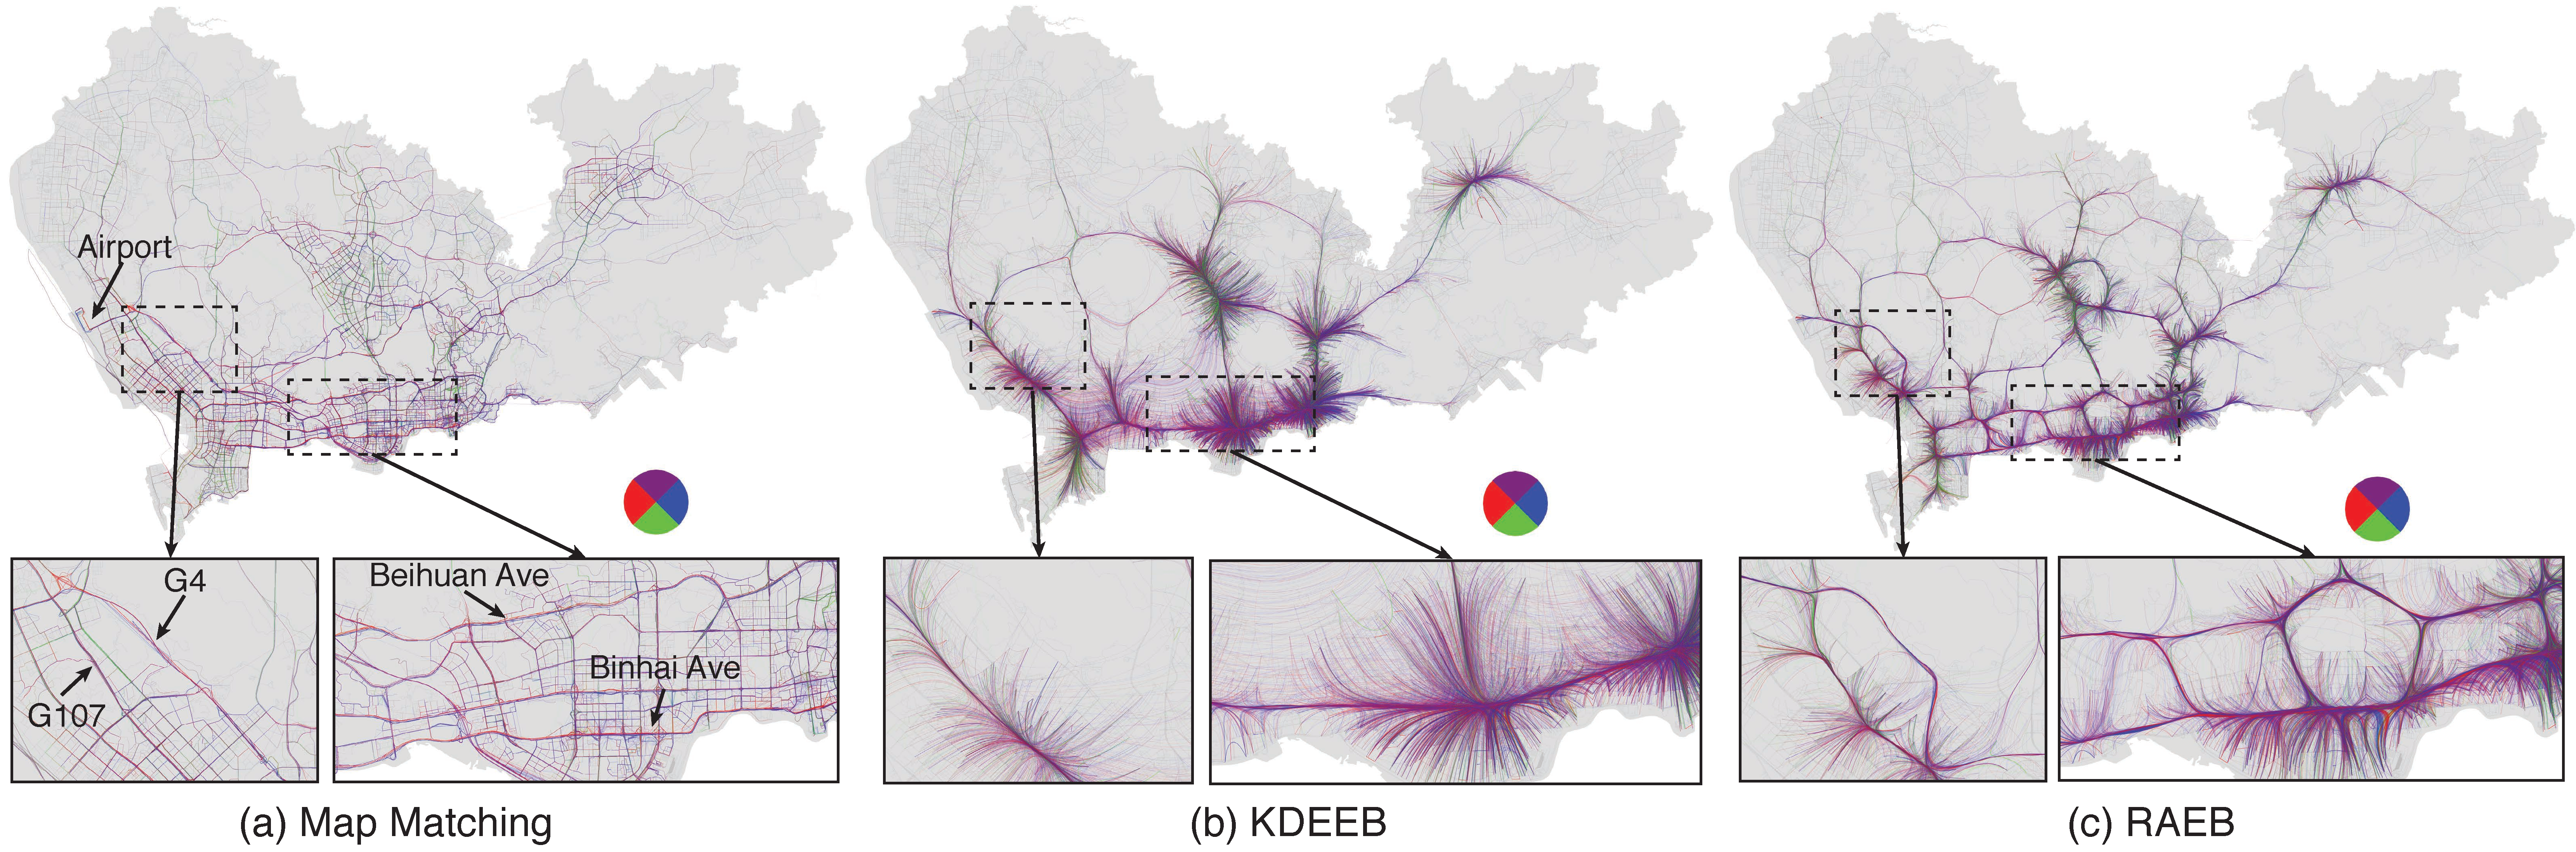
\includegraphics[width=0.995\textwidth]{fig10_study3/shenzhen}
	\vspace{-2mm}
	\caption{
	Density maps of Shenzhen taxi trips: (a) raw GPS records are mapped onto road network, (b) KDEEB bundles trips on close aterial roads together, while (c) RAEB preserves these roads. All lines are colored according to the OD directions.
	}
	\label{fig:shenzhen}
	\vspace{-4mm}
\end{figure*}

%%%%%%%%%%%%%%%%%%%%%%%%%%%%%%%%%%%%%%%%%%%%%%%%%%%%%%%%%%%%%%%%%%%%%%%%%%%%%%%%%%%%
\subsection{New York Taxi Trips}
\label{ssec:study2}

In reality, a road network is usually much more complex, and OD trails are more dynamic than the artificial ones.
In this experiment, we further compare RAEB with KDEEB using results generated from New York taxi trips.

The road network employed in this study is extracted from OpenStreetMap (OSM) within the boundary of Manhattan, Brooklyn, Queens, and Bronx zones, where most origins and destinations are located.
The raw network consists of 133,154 nodes, 166,122 edges, and it is simplified to 97,336 routes.
The OD trails studied in this experiment are 100K taxi trips extracted from one-month trip records.
The original records consist of various attributes for each trip, including vendor id, pickup \& dropoff times and positions, and fare amount, etc.
We use the pickup \& dropoff positions, and map it onto the road network using shortest path algorithm.
Figure~\ref{fig:nyc_visual}(a) presents a density map of the mapped taxi trips.

Figure~\ref{fig:nyc_visual}(b - d) show bundling results generated by KDEEB and RAEB, with graph drawing sizes set to 1080 $\times$ 1440.
The experiment is started with KDEEB recommended settings of kernel size $p_r$ = 60 (about 5\% of graph drawing size) and $p_n$ = 10.
Figure~\ref{fig:nyc_visual}(b) shows the bundling result, which clearly presents several main bundles.
The bundles reveal primary traffic movements over the whole city.
Yet in other ways, the results are heavily bundled, missing details of road network topology.
To show more details, we measure initial kernel size considering both graph drawing and geometric property of road network as described in Section~\ref{ssec:kernel_size}.
$p_r$ is reduced to 21.
Figure~\ref{fig:nyc_visual}(c) shows the corresponding KDEEB bundling results.
More bundles are formed, in line with arterial roads in New York.
However, there are many bundles lying by non-existing roads, as those shown in the highlighted region in-between Manhattan and Brooklyn.
This illustration can cause wrong impression of bridges connecting the zones.
Figure~\ref{fig:nyc_visual}(d) shows results generated by RAEB, with $p_r$ = 21 and route awareness $p_{ra}$ = 1.
The undesirable bundles are removed by our method.

Visualization of urban traffic should support multi-scale exploration $-$ an important characteristic for movement data visualization.
In the context of this work, a good edge bundling algorithm should provide smooth transitions of bundling results at different scales.
We further evaluate multi-scale exploration by zooming into the blue region in Queens zone as in Figure~\ref{fig:nyc_visual}(c) \& (d), and applying KDEEB and RAEB on the OD trails.
The fine scale bundling results are presented in Figure~\ref{fig:nyc-zoom}(a) \& (b), respectively.
More bundles are generated by both methods, as the same effect when zooming into maps.
However, it is difficult to visually match bundles in Figure~\ref{fig:nyc_visual}(c) with those in Figure~\ref{fig:nyc-zoom}(a).
In comparison, bundles in Figure~\ref{fig:nyc_visual}(d) can be more easily identified in Figure~\ref{fig:nyc-zoom}(d).

%%%%%%%%%%%%%%%%%%%%%%%%%%%%%%%%%%%%%%%%%%%%%%%%%%%%%%%%%%%%%%%%%%%%%%%%%%%%%%%%%%%%
\subsection{Shenzhen Taxi Trips}
\label{ssec:study3}

We further evaluate the performance of RAEB using taxi trips in Shenzhen, with road network extracted from OSM.
In total, there are 161K nodes and 177K edges, and the edges are simplified to 51K routes.
The OD trails are one-week taxi trip records.
Unlike New York taxi records with only origin and destination positions, Shenzhen's data contain a sequence of GPS positions recorded in every 20 seconds.
We clean and extract in total 50K taxi trips from the records.
The trips are further mapped onto the road network using ST-matching algorithm~\cite{lou_2009_map}.

Figure~\ref{fig:shenzhen}(a) presents a graph of the map matching results in the size of 2160$\times$1280.
The lines of a trip are colored according to direction from the trip's origin to destination.
The graph shows that most taxi trips are recorded in the southern region of Shenzhen, which borders on Hong Kong and is more developed than other regions.
The unevenly distributed taxi trips make it improper to use kernel size $p_r$ recommended by KDEEB, which is over 100 as 5\% of the graph drawing size.
Instead, our method suggests $p_r$ = 26, considering the road network topology as well.

Using this setting of $p_r$, both KDEEB and RAEB reaches stable states at iteration 8.
Figure~\ref{fig:shenzhen}(b) \& (c) show the corresponding results, respectively.
Both methods create smooth bundles in line with arterial roads in Shenzhen, indicating $p_r$ measured by our method is preferable.
Besides, nearly the same bundles are generated in regions other than south part, except that RAEB's result shows more details.
More dissimilar results are shown in the highlighted areas.
Expressways G4 and G107 lead traffic to Shenzhen airport in the left region, while Beihuan and Binhai avenues holds main traffic in the right one.
KDEEB merges OD trails passing these roads, while our method splits the bundles.
In short, RAEB generates results more similar to real-world scenarios.
\section{Discussion}
\label{sec:discussion}

The experiments demonstrate that RAEB outperforms KDEEB in visualizing OD trails in urban traffic data.
The first experiment with artificial data shows that the introduction of route awareness $p_{ra}$ in RAEB distinguishes grid and hierarchical network structures.
The second experiment presents the comparisons between KDEEB and RAEB using New York taxi data, which records only origin and destination positions. 
The results with different kernel size $p_{r}$ and in multi-scales indicate that, 
(1) $p_{r}$ should be measured based on not only graph drawing size, but also underlying road network topology;
and (2) RAEB supports better multi-scale exploration.
The robustness of RAEB is further demonstrated through the third experiment with Shenzhen taxi data, which records a sequence of GPS positions in every 20 seconds.

The advancements are achieved by parameter settings adopted in RAEB.
This section presents detailed discussion on the parameters, followed by performance comparison between RAEB and KDEEB. 
In the end, we discuss about generality and limitation issues.

%%%%%%%%%%%%%%%%%%%%%%%%%%%%%%%%%%%%%%%%%%%%%%%%%%%%%%%
\begin{table}[h]
	\begin{tabularx}{0.995\textwidth}{|>{\hsize=0.3\hsize}X|
			>{\hsize=0.18\hsize}X|
			>{\hsize=0.52\hsize}X|}
		\hline
		\textbf{Parameters} & \textbf{KDEEB} & \textbf{RAEB} \\
		\hline \hline
		Route awareness ($p_{ra}$)& $-$ & 0 - Number of road hierarchies\\
		\hline
		Kernel size ($p_r$) & Graph drawing & Graph drawing and road network geometry \\
		\hline
		Bundling iterations ($p_n$)& 10 - 15 & $-$ \\
		\hline
		Bundling stability ($p_{s}$)& $-$ & \textit{NMI} between images in consecutive iterations\\		
		\hline
		Bundling deviation ($p_{d}$) & $-$ & of bundles to OD trails\\
		\hline
	\end{tabularx}
	\caption{Main parameter adaptions in RAEB, in comparison with these in KDEEB.}
	\label{tab:parameters}
	\vspace{-1mm}
\end{table}

\subsection{Parameters}
\label{ssec:parameters}

RAEB adapts and introduces new parameters to better visualize OD trails in urban traffic data.
Table~\ref{tab:parameters} presents an overview of these parameter settings in comparison with those in KDEEB.

\begin{itemize}

\item
\textbf{Route awareness ($p_{ra}$):}
An input graph for KDEEB is straight lines connecting end nodes directly.
As discussed in the first experiment with artificial OD trails, such an input graph cannot distinguish grid and hierarchical road networks.
Instead, we introduce route awareness parameter $p_{ra}$ to control layout of input graph.
The first experiment also shows that $p_{ra}$ can be manipulated to generate bundles representing levels of details of road network.
If $p_{ra}$ is set to zero, input graph will be straight lines and the results are the same with KDEEB;
if $p_{ra}$ is set to the highest number of road hierarchies, input graph will be OD trails in line with road network, and more roads can be preserved.

\vspace{1mm}
\item
\textbf{Kernel size ($p_{r}$):}
In the second experiment with New York taxi data, we show that the parameter kernel size $p_r$ can control bundling coarseness.
KDEEB computes $p_{r}$ as 5\% of graph drawing size, which will generate coarse bundles that can only reveal main traffic connections (Figure~\ref{fig:nyc_visual}(b)).
Instead, RAEB suggests $p_{r}$ should be measured based on both graph drawing size and road network geometry.
In this way, a smaller $p_{r}$ is generated, and fine bundles that reveal details of street networks are generated (Figure~\ref{fig:nyc_visual}(c) \& (d)).
The advantage of our approach is further demonstrated using Shenzhen taxi data, which exhibits imbalanced distribution of taxi trips in the city.

\vspace{1mm}
\item
\textbf{Bundling iteration ($p_{n}$):}
KDEEB presets bundling iteration $p_{n}$ to a fixed number in between 10 - 15, such that to terminate the bundling process.
The choice of a suitable $p_{n}$, however, needs much experience and varies among different people. 
Adjustments in other parameters may also require fitting of the parameter.
RAEB discards this subjective parameter.

\vspace{1mm}
\item
\textbf{Bundling stability $p_{s}$:}
Instead, RAEB introduces a new parameter $-$ bundling stability $p_{s}$, to control bundling process termination.
$p_{s}$ is measured as normalized mutual information (\textit{NMI}) between images generated in two consecutive bundling iterations.
\textit{NMI} is a common metric in image processing field, thus can be easily integrated.
When $p_{s}$ reaches a predefined threshold, which means that visually a stable structure is generated, the bundling process will be automatically terminated.


\vspace{1mm}
\item
\textbf{Bundling deviation $p_{d}$:}
While $p_{s}$ measures bundling stability of a bundling method, it still lacks a method to quantitatively compare multiple ones.
The parameter bundling deviation $p_{d}$ is introduced to fill the gap.
$p_{d}$ is measured as average Frechet distance of bundles to corresponding OD trails.
The measurement is widely employed in geographical science, and we compare KDEEB and RAEB regarding the parameter below.

\end{itemize}

Some of these parameters can be automatically computed, including $p_r$ and $p_d$, while settings of $p_{ra}$ and $p_{s}$ can be consistent across different input data.
From the experiments, we recommend 1 for $p_{ra}$ (corresponding to top 5\% ranked routes), and 75\% for $p_{s}$.

%%%%%%%%%%%%%%%%%%%%%%%%%%%%%%%%%%%%%%%%%%%%%%%%%%%%%%%
\subsection{Performance}

\begin{table}[!tb]
	\setlength\extrarowheight{2pt}
	\begin{tabularx}{0.95\textwidth}{|
							  >{\hsize=0.19\hsize}X|
                              >{\hsize=0.16\hsize}X|
                              >{\hsize=0.05\hsize}X|
                              >{\hsize=0.17\hsize}X|
                              >{\hsize=0.13\hsize}X|
                              >{\hsize=0.17\hsize}X|
                              >{\hsize=0.13\hsize}X|}
	\hline
	Graph & Edge & $p_n$ & \multicolumn{2}{c}{Time (sec.)} \vline & \multicolumn{2}{c}{Deviation (pixel)} \vline \\
	& Samples & & KDEEB & RAEB& KDEEB & RAEB \\
	\hline \hline
	Random (grid) & 4.6M & 13 & 40.3 & 50.7 & 18.37 & 12.58 \\ 
	\hline
	NewYork & 3.1M & 11 & 34.3 & 42.9 & 15.40 & 9.88 \\
	\hline
	Shenzhen & 1.3M & 8 & 13.8 & 22.8 & 13.71 & 10.53 \\
	\hline
	\end{tabularx}
	\caption{Statistics comparison of KDEEB and RAEB for datasets used in the experiments. }
	\label{tab:statistics}
\vspace{-1mm}
\end{table}

Table~\ref{tab:statistics} shows comparison of KDEEB and RAEB for the datasets used in the experiments.
Both methods are implemented in Java running on a MacBook Pro with a 3.1 GHz Core i7 and Radeon Pro 560 graphics.
We employ the same kernel size $p_r$ and bundling iterations $p_n$ measured by our approach for both methods.

KDEEB's bundling process include sampling, splatting, advecting and smoothing steps.
Bundling time for each iteration is mainly determined by number of edge samples and kernel size.
Since kernel size measured by our approach is generally smaller than that by KDEEB, bundling time is reduced. 
The total running times for KDEEB methods are comparable with those in the original work~\cite{hurter2012graph}.
RAEB requires an additional step of bundling stability measurement, which is determined by the graph drawing size.
This adds in a running time of less than 1 seconds in each iteration for all three experiments.
The measurement is computed in every bundling iteration, thus we can shorten time by reducing the measurement frequency.
All the steps can be further accelerated using GPU e.g. CUDA~\cite{van2016cubu}.

On the other side, bundles generated by our method are more close to OD trials, as revealed by comparison regarding bundling deviation. 
From the table, RAEB reduces about 1/3 deviations of those in KDEEB for artificial and New York taxi datasets. 
The improvement is smaller for Shenzhen taxi data, though graph drawing in Shenzhen experiment is bigger.
This is probably because taxi trips are concentrated in a small area in the south of Shenzhen.
Nevertheless, the result image by RAEB shows more improvements than that by KDEEB (Figure~\ref{fig:shenzhen}(c) vs (b)). 


%%%%%%%%%%%%%%%%%%%%%%%%%%%%%%%%%%%%%%%%%%%%%%%%%%%%%%%
\subsection{Applicability and Limitations}
\label{ssec:app}

The experiments have shown the applicability of RAEB for bundling and visualizing OD trails in urban traffic using real-world taxi data.
RAEB introduces new parameters of route awareness $p_{ra}$ and bundling deviation $p_d$, and adapts existing measurement of kernel size $p_r$, to better fit road network topology.
The approach can be extended to other types of urban traffic data, such as commuter trips using public transportation, or people traces derived from call detail records.
These dataset consists of both OD trails and underlying road network.
Through advanced map matching algorithms, urban traffic's real paths on a road network can be recovered.
However, the parameters are not applicable to general graphs with information of only node connections, except for bundling stability $p_{bs}$.

Edge bundling methods face a common issue of unrealistic bundle lines.
Specifically for OD trails in urban traffic, bundle lines should not be far away from real paths.
RAEB mitigates the issue with route awareness $p_{ra}$ for controlling edge layout of input graph, and bundling stability $p_{bs}$ for generating stable results.
The first experiment shows that $p_{ra}$ can preserve certain routes on demand, while the second experiment reveals that RAEB supports better multi-scale exploration.
Experimental results of bundling deviations $p_{d}$ further proves the advantage of RAEB over KDEEB.
Nevertheless, these parameters can only constrain bundle layout in certain extent, as resulting bundle lines are still displaced from OD trials.
In scenarios requiring precise positions, such as query movements passing through a waypoint~\cite{kruger_trajectorylenses_2013} or road segment~\cite{wang_2014_visual-reasoning}, visual hints are required to remind the displacement.

Bundles generated by RAEB can show clear traffic patterns, meanwhile preserve road network topology better than KDEEB in a city.
These main goals of this work have been successfully achieved, as demonstrated by the experiments.
On the other hand, RAEB is not able to reveal detailed traffic patterns such as directional movements.
Direction is of recognized importance for studying OD trails in urban traffic~\cite{zeng_2015_visualizing}.
This limitation can be addressed by including directional information in density estimation or edge advecting functions, as described in CUBu~\cite{van2016cubu}.
Besides, RAEB is an image-based edge bundling method, constraining its applicability for 2D rendering only.
Applications such as to bundle movements~\cite{lambert20103d, thony2015vector} and fiber tracts~\cite{hurter_2018_functional} in 3D, and graphs in virtual reality~\cite{kwon_2016_study}, need spring- or geometry-based bundling methods.
\section{Conclusion and future work}
\label{sec:con}

OD visualization is challenging $-$ no universally good technique is available for visualizing arbitrary ODs~\cite{andrienko_visual_2012}.
In particular, this work studies OD trails in urban traffic.
We identify inconsiderate settings of existing kernel density estimation edge bundling (KDEEB) method when applied in the scenario.
This is because KDEEB was developed for general graphs such as airlines and migrations, while ignores data nature of urban traffic data.
These inconsiderate settings can cause domain-specific problems such as no preservation of road network topology and poor support of multi-scale exploration.
We contribute to the field with a new technique, namely route-aware edge bundling (RAEB). 
The bundling process is complemented with preprocessing that generate more proper input edge layout, and evaluation that create more stable visual results.
A series of parameter adaption and introduction are made to better cater to geometric properties of OD trails and road networks.
We compare RAEB with KDEEB in regarding to bundling time and deviation using artificial and real-world taxi data.
The experiment results show that RAEB outperforms KDEEB in reducing bundling deviation meanwhile achieving comparable computation speed.

Even though RAEB is specifically designed for bundling OD trails in urban traffic, some parameters such as bundling stability $p_{bs}$ can be applicable to other iterative edge bundling methods, including SBEB~\cite{ersoy2011skeleton} and FDEB~\cite{holten2009force}.
We would like to try integrating these parameters in the bundling methods, such that to make them more controllable.
We also realize many computation tasks in RAEB can be parallelized, thus bundling efficiency can be improved by GPU acceleration.
It would be worthy to reimplement RAEB in GPU, similar to CUBu~\cite{van2016cubu}.
Besides bundling control and efficiency issues, how to access bundling quality and faithfulness are the main challenges hindering the applicability of edge bundling methods~\cite{lhuillier2017state}.
Our experiences in developing RAEB suggest that in specific application scenarios, these challenges can be solved with domain knowledges.
On the basis of treating OD trails mapped onto road network as ground truth, our proposed parameter of bundling deviation $p_d$ is a quality and faithfulness metric in certain extent.
The parameters is derived from Frechet distance that is a common metric in geographical science.
In the future, we would like to apply RAEB in other fields such as to visualize neural connections in brain~\cite{2014_bottger_three-d, yang2016blockwise}.
Adaptions are most likely required, and we envision close collaborations with domain experts can facilitate the development.

% \chapter{Visual Interpretation of Recurrent Neural Network on Multi-dimensional Time-series Forecast}\label{chap:c3_intro}
Recent attempts at utilizing visual analytics to interpret Recurrent Neural Networks (RNNs) mainly focus on natural language processing (NLP) tasks that take symbolic sequences as input.
However, many real-world problems like environment pollution forecasting apply RNNs on sequences of multi-dimensional data where each dimension represents an individual feature with semantic meaning such as $PM_{2.5}$ and $SO_2$.
RNN interpretation on multi-dimensional sequences is challenging as users need to analyze what features are important at different time steps to better understand model behavior and gain trust in prediction.
This requires effective and scalable visualization methods to reveal the complex many-to-many relations between hidden units and features.
In this work, we propose a visual analytics system to interpret RNNs on multi-dimensional time-series forecasts.  
Specifically, to provide an overview to reveal the model mechanism, we propose a technique to estimate the hidden unit response by measuring how different feature selections affect the hidden unit output distribution. 
We then cluster the hidden units and features based on the response embedding vectors. 
Finally, we propose a visual analytics system which allows users to visually explore the model behavior from the global and individual levels.
We demonstrate the effectiveness of our approach with case studies using air pollutant forecast applications.


%!TEX root = ../article.tex
% \section{Introduction}
\section{Introduction}
\label{section:introduction}
Recurrent neural networks (RNNs) have been widely applied in various natural language processing (NLP) tasks such as machine translation and sentiment analysis. 
% Compared with other network architectures like fully connected networks, RNNs can effectively model sequential data.
Benefiting from the capacity to model sequential data, RNNs have been extended to other domains of sequential data beyond NLP, such as weather forecast\cite{xingjian2015convolutional, cao2012forecasting, shi2017deep} and air pollutant prediction\cite{oprea2016neural, zhou2017prediction, li2017long}. 
% and even stock market\cite{kim2018forecasting,nelson2017stock,akita2016deep}.
Compared to NLP tasks that take latent embeddings as inputs, the input features in these applications are usually multi-dimensional time series where each dimension has its own semantic meaning.
For example, in air pollutant forecast, RNN models are widely adopted by domain experts where input sequences are hourly recorded series of high-dimensional pollutants (\emph{e.g.}, $SO_{2}$) and meteorology features (\emph{e.g.}, \textit{wind speed}).
% After developing RNN models for forecasting air pollutant concentration, the domain researchers aim to further understand how RNNs model time-series data and if the model's behaviour is consistent with their domain knowledge, thus gain trust in prediction. 
% The time-series data in this application are sequences of hourly recorded high-dimensional vectors in which each dimension indicates a feature related to the air pollutant such as \textit{wind speed} or the concentration of $SO_{2}$.
% The sequence length ranges between 6 and 72 to record the historical data from the previous 6 to 72 hours.

Despite the competitive performance of RNNs, the lack of understanding of their internal mechanisms makes the models untrustworthy and further limits their extension to other domain applications. 
During model development, the domain experts usually want to better understand the models' forecast.
They tend to learn whether the model's behavior confirms any hypotheses according to existing domain knowledge, which helps gain confidence in prediction for decision making.
On the other hand, the experts also aim to identify the patterns that have not been observed before by exploring different cases to enrich their knowledge of the domain problem.
\UC{In addition, understanding RNNs also helps model designers to choose appropriate model architecture and hyper-parameters.}
% Understanding RNNs also helps model designers better choose models and tune hyper-parameters, adjust the model's architecture, and remove unnecessary features in the input space.
% unobserved -> unknown

% In this work, we are motivated by the requirements of air pollutant forecast. 
% The domain researchers have developed RNN models to forecast the concentration of air pollutants.
% They aim to understand how RNNs model time-series data and if the model's behaviour matches their domain knowledge, thus increasing confidence in the models. 
% The time-series data in our application are sequences of hourly recorded high-dimensional vectors in which each dimension indicates a feature related to the air pollutant such as \textit{wind speed} or   
% the concentration of $SO_{2}$.
% The sequence length ranges between 6 and 72 to record the historical data from the previous 6 to 72 hours.


% Existing work on RNN interpretation such as mainly focuses on NLP tasks. 
% For example, LSTMVis~\cite{strobelt2018lstmvis} uses parallel coordinates to visualize the periodic patterns of hidden states in order for experts to verify their hypotheses.
% RNNVis~\cite{ming2017understanding} models the input text and hidden units as a bipartite graph and uses co-clustering techniques to cluster the hidden units and text simultaneously to present more structural information learned by the model. 
% Both of these two works interpret hidden units by providing their relevant words as language contexts.
% However, existing techniques cannot be directly applied in RNNs for high-dimensional time-series forecasts.
% \UC{Merge with the next paragraph}

Existing work on RNN interpretation such as LSTMVis~\cite{strobelt2018lstmvis} and RNNVis~\cite{ming2017understanding} mainly focus on NLP tasks. 
Both of these two works interpret hidden units by providing their relevant words as language contexts.
However, existing techniques cannot be directly applied in RNNs for high-dimensional time-series forecasts.
First, the high dimensionality of the input sequence makes it difficult to discover relationships between features and hidden states. 
Since different features at various timestamps are correlated, traditional techniques are not applicable as they are not designed to reveal how feature importance changes over time, which hinders the domain experts' ability to analyze if the prediction is consistently generated.
Analyzing this complex temporal multi-dimensional data requires an effective visualization design that can reveal both cross-dimension data relationships and the model's temporal behavior.
Moreover, in real-world applications, the input dimension size may be from hundreds to thousands, and the hidden unit size of the RNN models can also be large.
This requires the visualization methods to have good scalability in order to demonstrate the distribution and complex relationships of hidden units and input features.
% \zw{try to illustrates challenges using our domain words like spatio-temporal, multi-dimensional, multi-scale, comparative.}

% Second, as RNN models capture and utilize the temporal sequence information for prediction, the hidden states are affected by both the features at current time step and the hidden units from previous time steps. 
% This adds an additional complexity in both interpretation and system scalability.


% To address these challenges, We propose a visual analytics system to help domain experts to understand RNN in high-dimensional time series forecast tasks by uncoverng the relationship between input features and hidden states. 
% Specifically, we develop a co-clustering view (\zw{Fig.~\ref{fig:teaser}(xxx)?}) to visualize the relations between hidden units and input features and support flexible interactions to allow users focusing on interested features or feature value ranges.
% We also propose a sequence view (\zw{Fig.~\ref{fig:teaser}(xxx)?}) to summarize and compare the temporal hidden unit and feature importance along the sequences with good scalability.

\UC{To address these challenges, we propose MultiRNNExplorer, a visual analytics system to help domain experts understand RNNs in high-dimensional time-series forecasts from two aspects: model mechanism and feature importance. 
To understanding model mechanism, we estimate the overall response from hidden units to features and generate response embedding for both hidden units and features.
We then cluster the hidden units and features respectively to reveal the high-level knowledge captured by the models.}
To measure the feature importance, we calculate the gradient for all features at all timestamps with respect to a given case.
% To facilitate case-based exploration, we use gradient-based techniques to measure the feature importance.  The gradients at all timestamps are calculated for all cases to measure the local importance of features. 
Then a visualization interface with coordinated views is designed, enabling the users to interactively explore the model behavior. 
% Specifically, we design a Cluster View (Fig.~\ref{fig:teaser}A) to visualize the hidden units' response to features. 
% The hidden units are visualized in a distribution chart and the features are visualized as a glyph. Then the Feature Importance View (Fig.~\ref{fig:teaser}C) summarizes the temporal importance of all features. Finally, the individual level behaviors of RNNs are visualized in a \UC{Individual View} (Fig.~\ref{fig:teaser}D) which visualizes the feature trend, cluster importance trend and the top features for each individual case.

Our contributions can be summarized as follows:
\setlist{nolistsep}
\begin{itemize}[noitemsep]
%   \itemsep0em 
  \item \UC{A new method for estimating neuron response to multi-dimensional time-series data by measuring hidden unit response distribution on different value ranges of input features.}
  \item A visual analytics system that help users to explore, interpret, and compare RNNs on multi-dimensional time-series data. 
  \item Several case studies on air pollutant datasets to demonstrate the effectiveness of the proposed system and the insights revealed during exploration.
\end{itemize}






%!TEX root = ../article.tex
\section{Related Work}
\label{sec:rel}

\subsection{Recurrent Neural Networks}
\label{sec:rnn}
Recurrent Neural Networks (RNNs) is a class of neural networks that contains feedback connections~\cite{hochreiter1991untersuchungen}.
Compared with fully connected neural networks, this architecture is capable of processing temporal data and learning sequences.
Many RNN variants have also been developed in the past decades.
One typical work is Long-Short Term Memory (LSTM)~\cite{hochreiter1997long}.
By integrating several gate functions and appending an additional cell state to the vanilla RNN, LSTM avoids the gradient vanishing problem when processing the long sequences.
A similar but computationally more efficient approach is the Gated Recurrent Unit (GRU)~\cite{cho2014learning}, which simplifies the model architecture by using only two gate functions: update gate and reset gate.
To better utilize more data along the sequence, the bi-directional RNN~\cite{schuster1997bidirectional} is proposed to capture both past and future information to improve prediction.
Greff et al. proposed a comprehensive survey~\cite{greff2017lstm} to summarize and compare these RNN variants in order to guide model selection under different scenarios.

RNN-based models have not only been proven successful in performing Natural Language Processing (NLP) tasks such as machine translation~\cite{sutskever2014sequence} and question answering~\cite{hermann2015teaching}, but have also been adopted in broader domains such as weather forecasting~\cite{xingjian2015convolutional} and environmental factor prediction~\cite{chen2018applications}.
For example, Oprea et al. proposed an RNN-based architecture to forecast $PM_{2.5}$ air pollutants~\cite{oprea2016neural}.
Compared with the NLP domain, these critical areas not only require good model performance but also need humans to understand how a prediction is generated and whether the results are trustable for guiding further decision makings~\cite{lipton2017doctor}.
However, understanding RNNs in such scenarios is challenging.
On the one hand, as each input dimension is usually informative and usually indicates an interpretable factor compared with word embeddings used in NLP, analyzing which features have the most impact on prediction results is important.
On the other hand, users also need to explore and understand how the hidden states evolve over time in order to reveal the underlying working mechanism of the RNN along the sequence.
We propose MultiRNNExplorer to better understand and interpret RNN models, especially when the model input is multi-dimensional as with the above critical areas.

\subsection{Machine Learning Interpretation}
\label{sec:mlinter}
In recent years, many machine learning interpretation methods have been developed, which can mainly be categorized into two groups: model reduction and feature contribution.

Model reduction methods usually learn a surrogate model to approximate the original complex model.
The surrogate model is usually simple and interpretable, such as linear regression~\cite{ribeiro2016should} and decision trees~\cite{craven1996extracting}. 
Depending on the ways of approximating the original model's behaviors, there are three main ways to conduct model reduction: decompositional, pedagogical, and eclectic~\cite{andrews1995survey}.
Decompositional methods are usually model dependent and simplify the original model structure, such as the layer and weights of the neural network.
Pedagogical methods only utilize the input and output information to mimic the original model.
Eclectic methods are either a combination of the previous two approaches or are distinctively different from them.
Though model-reduction-based methods are flexible and easy to understand, it is questionable whether or when the surrogate model truly reflects the original model's behaviors.
We thus discard this approach in our work.

Feature contribution methods help users understand the relationships between input features and the output prediction.
They usually assign each feature an importance score to indicate how it impacts the final prediction.
One classical work is Partial Dependence Plot (PDP)~\cite{friedman2001greedy}, which depicts how feature value changes affect predictions.
A PDP is usually visualized as a line \textbf{}chart in which the x-axis represents feature values and the y-axis represents prediction possibilities (partial dependence scores).
For each feature, its partial dependence scores are usually calculated by iteratively fixing the feature input of all the data points to a certain value and getting the average prediction.
One recent work, SHAP~\cite{lundberg2017unified}, also calculates feature attribution, but from a local perspective.
SHAP is based on the ideas of Shapley Values from game theory, which calculates the feature contribution of a data instance by comparing it with a set of reference data points.
Compared with global solutions, it is more consistent and locally accurate.
One major limitation of feature contribution methods is is that they are computationally expensive.
In this work, we alleviate this problem by adopting a pre-processing stage before interactive exploration.

Apart from the above work that focuses on describing the input-output relationship,
some work focuses on understanding and analyzing the internal working mechanism of RNNs, especially the hidden layer behaviors, by utilizing visualization techniques.
Karpathy et al. first conducted some explorative studies on hidden cell activation on different sequence items~\cite{karpathy2015visualizing}.
LSTMVis~\cite{strobelt2018lstmvis} further analyzed and compared the activation changes of each individual cell to demonstrate that different cells may capture different language patterns over time.
Ming et al. developed RNNVis~\cite{ming2017understanding} to depict the co-clustering patterns between hidden states and input words.
There is also some other work that focuses on a particular model or domain.
For example, Seq2Seq-Vis~\cite{strobelt2019s} mainly focuses on the sequence-to-sequence model and RetainVis~\cite{kwon2019retainvis} enables experts to analyze electronic medical data using a RNN model.
Though these methods show how the relationships between hidden units and input data change over time, they fail to capture the importance evolution of each individual input dimension, which prevents them being adopted in critical areas such as finance and environmental factor forecasting.
We aim to solve this problem by revealing the activation sensitivity of hidden units to different features and highlighting what features mostly affect the final prediction the most over time.


\section{Application and Models}
\subsection{Application}
\label{section:application}
In this paper, we focus on a particular type of regression task on multi-dimensional time-series data: air pollutant forecast of \textbf{target pollutants} at \textbf{target locations}.
We collaborate with a group of domain researchers who use RNNs to conduct air pollutant forecasting.
Specifically, they choose 16 air quality monitoring stations in Hong Kong with the stations' locations as the \textbf{target locations} and select $PM_{2.5}$, $PM_{10}$, $NO_{2}$, $SO_{2}$, and $O_3$ as the \textbf{target pollutants}.
Though the RNNs can provide high accuracy, the researchers are more interested in understanding why the models make certain predictions so that they can decide whether to trust the models for decision making based on their domain knowledge.
% \zw{needs more details here. analytical goals come too late. move here?}
We thus develop MultiRNNExplorer to help the domain researchers explain the RNNs' behavior on their temporal multi-dimensional air pollutant dataset.


% According to the requirement, for each model, on of the 16 air quality monitoring stations at Hong Kong as are chosen as\textbf{ target station}. 
% \yh{We may only describe our task and end users in Sec. 3.1 and remove other materials.}
% Our targeted problem is understanding RNN behaviour in air pollutant forecast. 
% The air pollutant has raised more and more attention of researchers. 
% As one of the most studied problems, traditional techniques such as CMAQ(Community Multi-scale Air Quality)~\cite{byun1999science} and ADMS-Urban~\cite{stocker2012adms} have been developed for long time air quality forecasting.
% However, the accuracy of these techniques relies on an updated pollutant source list which is very difficult to produce and update ~\cite{xi2015comprehensive}.
% Machine learning techniques are applied in this task~\cite{zhou2017prediction, reddy2018deep, ong2016dynamically} for the precise short-term prediction since it can leverage the real-time observation data. 

% \QM{Here we need to discuss the end user? This paragraph should be modified.}

% With the fast development of machine learning tools such as Tensorflow, Keras, Pytorch and Caffe, it becomes easier and easier for the environment researchers with no deep knowledge of machine learning to design and train models for the forecasting tasks. 
% Strobelt et al.\cite{strobelt2018lstmvis} has summarized three users roles: architects, trainers and end users. Our target users is between the trainer and end user. They utilize RNNs as tool and have domain knowledge about the atmosphere and air quality. They want to explore what the model learn and exam if the model capture reasonable factors to the forecasting.   



\subsection{Data Description}
\label{section:datadescription}

The dataset includes hourly observations of the air pollutant and meteorology data from different air quality monitoring stations in China from Jan. 01 2015 to Dec. 31 2018.
The features are listed in Table ~\ref{table:feature_list}.

\begin{table}[h!]
\centering
\caption{There are two types of features taken as input: air pollution and meteorology. }
\begin{tabular}{|p{2cm}|p{5.2cm}|} 
\hline
 Category & Feature type \\ [0.5ex] 
\hline
    Air pollutant&$PM_{2.5}$, $PM_{10}$, $NO_{2}$, $NO_{x}$, $SO_{2}$, $CO$, $O_3$\\[0.4ex] 
\hline
    Meteorology&\textit{Wind Speed(Wind), Wind Direction(WD), Dew Point(DP), Relative Humidity(RH), Temperature(Temp), Sea Level Pressure(SLP), Station Pressure(SP), Cloud Cover(CC)}\\
\hline
\end{tabular}
\label{table:feature_list}
\end{table}

% Since the monitoring stations which are too far away from the target locations have very few influence to the target location, the model only takes the observations from nearby stations as the input.
% Furthermore, even the spatial distance of the neighbor stations are limited, if all observations are fed into the model directly still cause trouble in the training and prediction with limit training data because the features collected from the stations may be redundant. 
Similar to other work on air pollutant forecasts~\cite{zheng2015forecasting}, when forecasting the air pollutants at a target location, we divide the regions around the target location into different spatial partitions and aggregate the data observed by all the stations within each group in order to generate features.
% Inspired by~\cite{zheng2015forecasting}, a similar spatial partition method are applied to aggregate the observation features(~\QM{as Fig.\ref{fig:teaser} B}). 
% \yh{Above sentences may be confusing...need discuss}
Specifically, as shown in Fig.~\ref{fig:teaser}B, we divide the nearby regions into five non-overlapping rings centered at the targeted location with radii of 10km, 30km, 100km, 200km, and 300km.
Each ring is further divided into 8 sectors with the same angle such that the whole area around the target location is partitioned into 40 sub-regions. 
For each sub-region, we use the air pollutant and meteorology data observed by the monitoring stations located in the corresponding sub-region as the features.
If there are multiple monitoring stations in a sub-region, we aggregate their data and use mean values as the features.
% The same features from the monitoring station located into a same region within a same time range(e.g. 1 hour) will be averaged by mean value of this region. 
In this way, each feature can be identified as a triplet $(distance, direction, feature\_type)$; for example, $(10km, E, NO_{2})$ indicates $NO_{2}$ concentration observed at \textit{10km} away \textit{East} of the target location. 
For each time step, we use a vector to represent all the features where each dimension indicates a feature triplet.
In this way, the data within a time peroid can be represented as a multi-dimensional sequence. 
% \QM{For each timestamp, we format all of the aggregated features at same timestamp as high-dimensional data and the data within a time range as a high-dimensional sequence.}

\subsection{Models Description}
\label{section:model_description}
RNNs take a sequence as input with fixed length $T$: $\{x_0, x_1,... x_{T-1}\}$ and predict the value at timestamps equal to or greater than $T$, where $x_{t} \in \mathbb R^{m}$. 
% To train and test the model, we use a sliding-window method with the window size between 6 and 48 to gradually scan all time-series data.
% \UC{So in the testing process, the input data $x$ will be read $T$ times and generate $T$ outputs from the hidden units.}
% \yh{To me, above 2 sentences describe how we generate sequences from data and can be removed / or moved to the data description sec.. I feel it is not direcctly relevant to model description.}
% and $x_{t}^k \in x_{t}$ is the value of $k^{th}$ at time-stamp $t$. Each dimension of $x$ are scaled in the range of [0, 1]. 
A hidden state $h_t$ is updated according to the input of timestamp $t$ and previous hidden state $h_{t-1}$.
\QM{In vanilla RNNs, the hidden states are updated by:} 
\begin{equation} 
h_t = \sigma(Wh_{t-1} + Vx_t)
\end{equation}

Where $W$ and $V$ are weight matrices and $\sigma$ is the $tanh$ function which constrains the output of the hidden states to $(-1, 1)$. We consider three types of architectures shown as Fig.~\ref{fig:model_type}. 
\textbf{RNN}: the final timestamp hidden state is directly connected to the output layer (Fig.~\ref{fig:model_type}A). \textbf{RNN-Dense}: there are several dense layers between the final timestamp and output layer (Fig.~\ref{fig:model_type}B). 
% In model of Fig.\ref{fig:model_type}A, the final time-stamp hidden state is directly connected to the output layer. For the model of Fig.\ref{fig:model_type}B, there are several dense layers between the final time-stamp and output layer. The model of Fig.\ref{fig:model_type}C has time-distributed dense layer between the RNN layer and output layer. In theory, the time-distributed layer can better capture the temporal dynamics\cite{teijeiro2017arrhythmia}.
In addition to vanilla RNNs, we also consider two variants: GRU and LSTM, which mitigate the gradient vanishing issue and enable the models to memorize long-term information by adding the ``gating'' mechanism.


\begin{figure}[t]
	\centering
    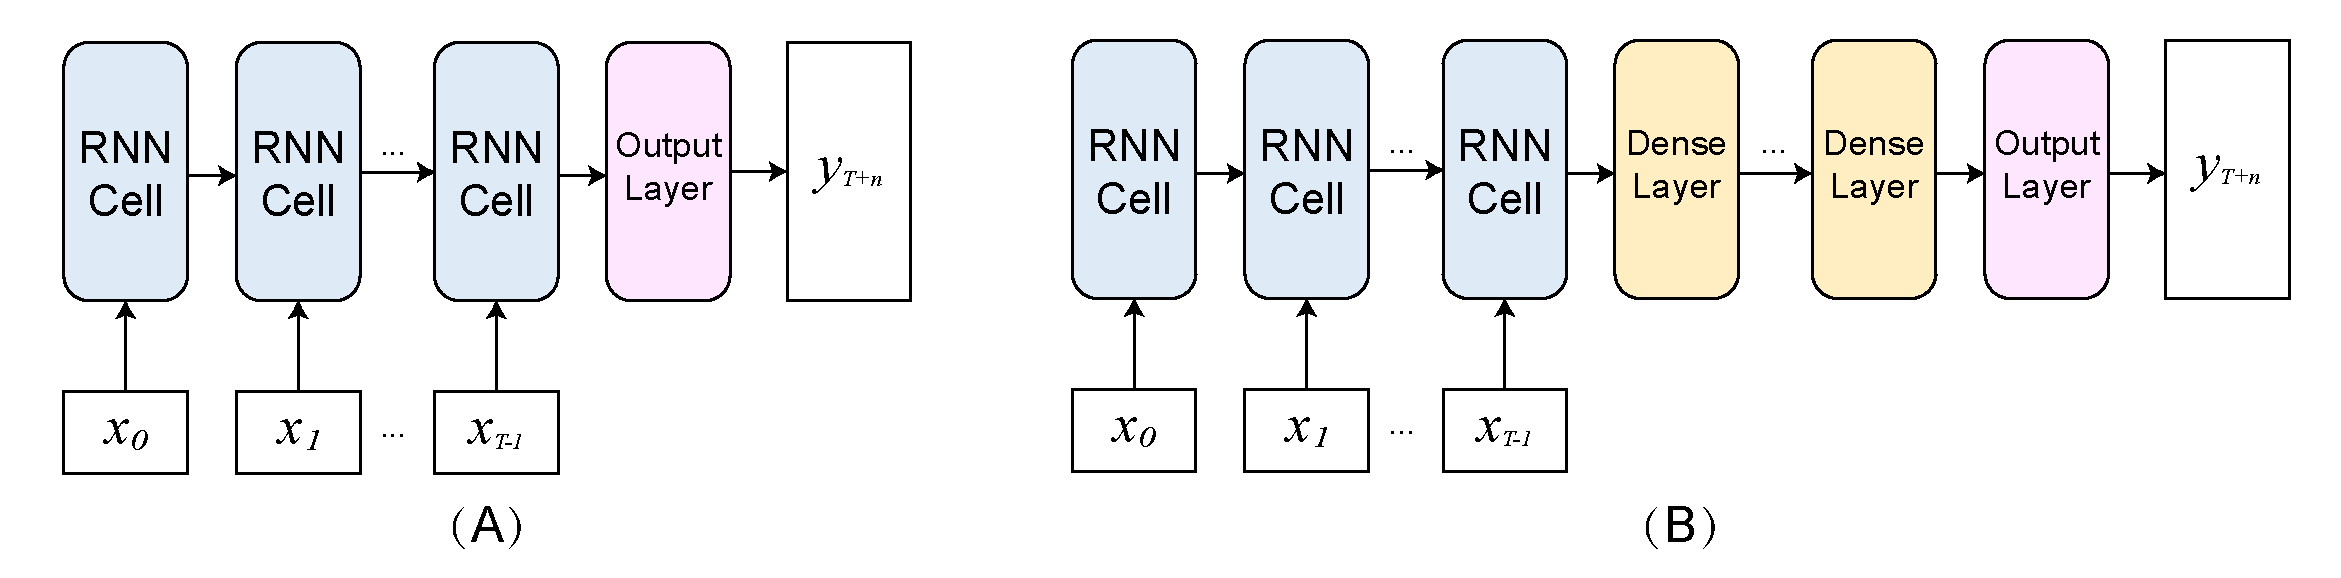
\includegraphics[width=0.9\textwidth]{figure/MultiRNNExplorer/model_description/model.pdf}
	\vspace{-5mm}
	\caption{\UC{RNN Architectures considered in our experiments: A) RNN: the RNN layer is directly connected to the output layer; B) RNN-Dense: adding dense layers between the RNN layer and the output layer.}
	}
	\label{fig:model_type}
\end{figure}


\section{System design}
In this section, the requirement and tasks are discussed. Over the past 12 months, we closely worked with two domain researchers in urban air quality analysis and forecasting. 
One researcher \UC{(R1)} studies the atmospheric diffusion of air pollutants and has interest in what machine learning model learns.
The other researcher (R2) is working on air pollutant forecasts through machine learning techniques. Both of them have strong domain experience in air quality forecasting. 

% \subsection{Analytical  Goals}
% We have distilled the following goals based on an informal interview with domain experts who work on utilizing RNN models to predict weather pollution. 
\subsection{Task analysis}

During the discussions, three general goals were distilled:
G1: Understand the RNN model behavior/mechanism in high-dimensional forecasts. 
G2: Understand the feature importance. 
G3: Support case-based exploration.

% \textbf{G1: Understand the RNN model behavior/mechanism in high-dimensional forecasts.} 
% Since the target users already have basic knowledge about the RNN models including their structure and theory, the crucial requirement to understand the model is to explain how such structure works for the forecasting tasks. 
% For example, how do the hidden units capture the information from the time-series data? 
% Understanding the hidden units is challenging because of the complicated many-to-many relationship which exists among hundreds of hidden units and features. 
% Compared with tasks related to natural language or image processing, it is difficult to extract semantic information from  high-dimensional time-series data. 
% An effective way to calculate, summarize, and visualize the relationship as well as the high-dimensional time-series data is required. 

% \textbf{G2: Understand the feature importance.} 
% Unlike R1, the feature importance explains the machine learning model by considering the model as a black box. 
% In general, the feature importance measures the contribution of features to the forecasting result and can be effectively understood by the end user who has rich domain knowledge. 
% In this discussion session, the domain experts are extremely interested in which features always have a large contribution to the output while some of the features influence the result only under specific conditions. 
% Understanding the feature importance reflected by deep learning models can increase the trust of the end users or allow the users to justify the result.  
% Existing techniques include back-propagation-based approaches and perturbation-based forward-propagation approaches. 
% However, most of these methods target calculating the feature importance/contribution at the individual level and fail to provide an overview across all the features.  

% \textbf{G3: Support case-based exploration.} 
% Case-based exploration is one of the most effective strategies for humans to interpret machine learning models. 
% It is based on the assumption that a new problem can be resolved by the solutions of previous similar problems, which can serve as a scaffold for understanding the challenges. 
% Adopting case-based exploration can facilitate users in obtaining an overview of RNN models such as observing which types of data the model tends to make errors or identifying the most critical features that can affect a prediction. 
% Users can compare two similar sequences to see if the model performance is consistent or examine the predictions at consecutive time steps to estimate when the model's behavior changes dramatically. 
% However, providing case-based exploration for RNN models is challenging as the system needs to flexible enough for users to filter and search the cases of interest. 
% To examine a case, which consists of high-dimensional vectors from multiple time steps, the system is also required to be scalable and able to provide informative memorization at the same time. 
% We aim to provide users a flexible and effective case-based exploration workflow.

% \subsection{Design Tasks}
\label{section:design_tasks}
To fulfill the these analytics goals, we have specified the following analytical tasks:

\textbf{T1: Encode hidden state statistics.}
Hidden states, a direct reflection of a model's intermediate results, are critical for revealing the information captured by a model (\textbf{G1, G2}).
Visualizing hidden state statistics can provide a holistic picture of a model's capacity and behavior.
% By linking the hidden state activeness with data and prediction results, users can also identify the blind points where models tend to predict incorrectly.
% Thus, our system should support encoding various hidden state statistics such as value distribution and the data coverage.

\textbf{T2: Measure and encode feature importance at multiple scales.}
% The appropriate technique should be embedded in the system to measure feature importance. 
% Also, 
The visual analytics system should allow users to explore feature importance at different scales(\textbf{G2}). 
For example, the overview level ranks and presents feature importance summarized from the whole dataset. The individual level will focus on importance of single case.
% The group level exploration enables users to select a subset of cases and explore the feature importance distribution, while the individual level will focus on the feature importance of the single case.


\textbf{T3: Analyze the response between features and hidden states.}
Measuring the response relationship between features and hidden states is the key factor in revealing what patterns are captured by the model (\textbf{G1}). 
% By inspecting what features can activate certain hidden units, users can know how the model pays attention to different factors. 
% This also enables users to see if the model has utilized all the features or only focus on the most important ones. 
% In addition, 
Targeting at the complicated many-to-many relationship, the hidden states as well as the features should be clustered to alleviate the burden on end users. 


\textbf{T4: Support temporal analysis.}
One major advantage of RNNs is that they can capture time-dependent sequence information.
% The prediction is affected not only by the features from the last time step, but also the historical information being passed along the sequence.
Showing what information is preserved along the sequence and what information is discarded helps users better understand how the temporal information is utilized by the model(\textbf{G2, G3}).
In addition, users can identify the most critical time step that causes a significant change in the model's prediction.
% For these reasons, the system should be able to support temporal analysis when interpreting the model's behaviors.

\textbf{T5: Identify data clusters and outliers.}
To support case-based reasoning, users need to first obtain a data overview by identifying the data clusters and outliers (\textbf{G1, G3}).
This provides concrete examples to guide users in further exploring the data of interests.
% For example, users can estimate how many categories of data share the same or similar prediction results by observing data clusters.
Users can also inspect the outliers that have distinct prediction results to detect if the model behaves incorrectly according to certain domain knowledge.
% We aim to provide users an overview of the data and enable them to compare different data and their resulting predictions.

\textbf{T6: Explore the case-based model behaviour.}
The system needs to enable the users to explore how a model behaves for individual cases such as build the correlation between feature trend and feature importance trend(\textbf{G3}). 
Since hundreds of temporal features are taken as input for each case, the effective summary is required.


% \textbf{T6: Enable case comparison.}
% As the key concept of case-based exploration is to use existing knowledge to solve similar new problems, enabling sequence comparison is necessary for interpreting RNN models (\textbf{R1}). 
% Many scenarios require users to compare the prediction processes of multiple sequences at the same time.
% For example, users may need to examine two similar but slightly different sequences to identify at which time steps the model behaves differently.
% Conversely, users may also compare multiple sequences with similar prediction results to identify their common features.
% Therefore, the system needs to enable sequence comparison in different perspectives including both the hidden states and raw features.


% \textbf{T7: Support interactive model exploration}.
% All the tasks listed above require the system to provide interactive model exploration.
% For example, users may filter certain hidden states and want to inspect the features that can only activate these selected hidden states.
% Users may also need to select a few interesting sequences for comparison and focus on certain time steps.
% These requirements need the system to support a set of interactions for interactive exploration.

\subsection{System Overview}

\begin{figure}[t]
	\centering
    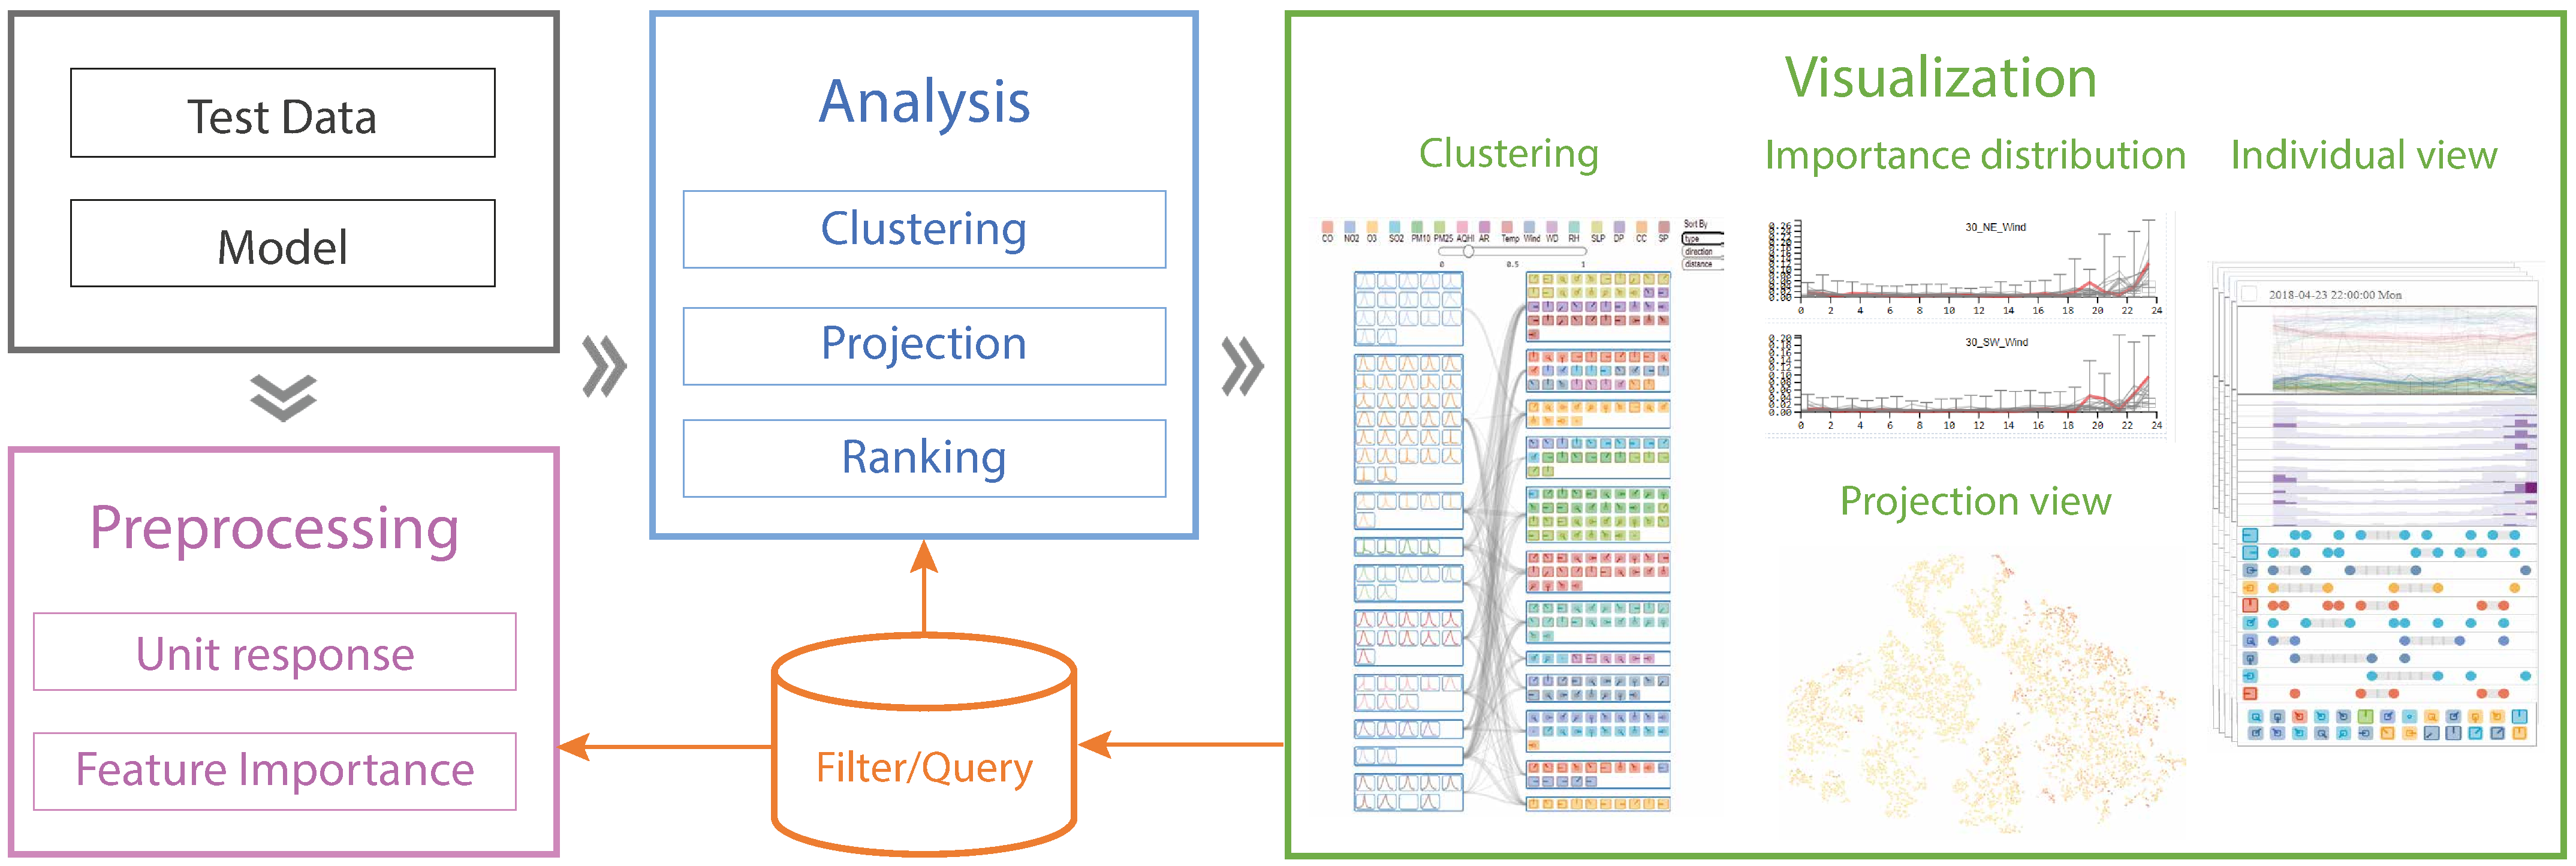
\includegraphics[width=0.95\textwidth]{figure/MultiRNNExplorer/System_framework.pdf}
	\vspace{-3mm}
	\caption{The system overview. There are three major modules in our system: Preprocessing module, Analysis module and Visualization module. 
% 	The preprocessing module estimates the hidden unit response and calculate the feature importance; the analysis module discovers patterns of the model's behaviors; the visualization module provides interfaces for the users to explore the model behavior.
	}
	\label{fig:system_framework}
	\vspace{-4mm}
\end{figure}


We implement MultiRNNExplorer as a web-based system using Flask, VueJS, and D3. 
The system consists of three modules: 1) preprocessing, 2) analysis, and 3) visualization.
% With chosen models, the preprocessing module is responsible for providing the raw data that need to be analyzed, including extracting hidden states and generating feature importance estimated from the testing data.
With chosen models, the preprocessing module generates the raw data that need to be analyzed, including estimating the response relationship and feature importance.
% extracting hidden states and generating feature importance estimated from the testing data.
We then apply various data analysis techniques such as clustering, projecting, and ranking in the analysis module to provide the data structure required by the visualization module.
The visualization module integrates coordinated views to support interactive interpretation of and reasoning about the model behavior at different perspectives. 

% \UC{need to move to design part.}
% The cluster view summarizes the hidden units' response to features.
% The projection view projects the individual cases by using t-SNE, which provides the users an overview of all individual cases.  This view also allows users to find and select cases of interest for further analysis.
% The importance distribution view shows the feature importance by timestamps. The ranking of the general importance will be updated according to the selected individual cases.  
% The sequence view enables users to explore the data at an individual level including the feature trend, cluster importance and the top features. 
% A rich set of interactions are also supported to link different views together.


% In this section, the system overview are discussed as Fig ~\ref{fig:system_framework}. The whole system consists of three components: model manager, model interpreter and visualization. 

% The model manager is designed to manipulate trained models and enable users to select the dataset they are interested in. With a choosing model and dataset, the model manager will manage the input data, output of each hidden states, and the gradient of input with respect to the hidden states output into the files.    

% With the output of model manager, then the model interpreter calculates the distribution of hidden states output first. Then it extracts the correlation graph by analyzing the difference of these distributions. At last, the model interpreter discover the dependency relations between the hidden state through the input gradient which will be discussed in section 5. 

% The distribution, correlation graph and dependency table will be finally provided to the visualization module. The visualization~\ref{fig:teaser} has six components, the control panel enable users to select the test data, trained model and configure parameters. The cluster view visualize the overview relationship between the variables and hidden units, users are allowed to interactively verify if a pattern is captured by the RNN model. The projection view projects the filtered sequence by using tsne which allow users identify how the hidden states are able to \QM{distinguish the different patterns}. The sequence view enable users to explore the data at individual level, where the temporal dependency between each hidden states and the dependency between the hidden states and input data will be visualized. All views are linked when common items are selected. 


\section{Model Interpretation}
This section first describes how we analyze the relationships between features and hidden states (\textbf{T3}).
Specifically, we propose an efficient method to calculate how sensitive each hidden state is to certain feature changes and apply a clustering method to group response relationship patterns for better scalability.
This provides users an overview on how the model categorizes different features and perturbing features to what value ranges may largely affect model behaviors.
We also introduce a gradient-based method to identify the most important features that can impact the prediction over time (\textbf{T2, T4}).
This provides another perspective on analyzing how feature importance changes along the sequence.
These two approaches are complementary to each other in enabling users'  understanding and explaination of model behaviors.

\subsection{Relationships between Hidden States and Features}

To measure how feature changes can affect hidden states (\textbf{T4}), one common approach is perturbing feature values and measuring how the hidden state distribution changes compared with the original data.
However, perturbation-based methods are usually time-consuming and not applicable when different features are correlated.
Inspired by~\cite{sun2015deeply}, we adopt another method that directly compares the hidden state distributions of different feature value ranges.
This approach is computationally efficient and provides a good approximation for whether a hidden state is sensitive to feature changes.
This section introduces how we generate the hidden state distribution for different value ranges of each feature and how we quantitatively measure the relationship strength between features and hidden states based on the generated distribution.

\subsubsection{Hidden State Distribution}
\label{section:response_and_activation}

As discussed in Sec.~\ref{section:datadescription}, the model input is a sequence of features $X=\{x_0, x_1, ..., x_{T-1}\}$ where $x_t$ indicates a multi-dimensional feature vector at time step $t$. 
Each feature dimension is denoted as $x_t^f$ in which $f$ represents a feature triplet $(distance, direction, feature\_type)$ at time step $t$.
Similarly, we use $H=\{h_0, h_1, ..., h_{T-1}\}$ to indicate the hidden state sequences at different time steps where $h_t = \{h_t^0, h_t^1, ..., h_t^{D-1}\}$ indicates the hidden state distribution at time step $t$ and $D$ denotes the hidden unit size.
As $h_t$ is computed by feeding $x_t$ into an RNN model $L$, we denote $h_t$ = $L(x_t)$.
Considering a dataset  $\mathbb{X} = \{X_0, X_1, ..., X_{N-1}\}$ consisting of $N$ sequences, we can collect a feature vector set $\mathbb{V} = \{x~|~x \in X, X \in \mathbb{X}\}$ where $|V| = N \times T$. 
Based on the value ranges of a feature $f$, we can further divide $\mathbb{V}$ into different groups $\mathbb{V}_g^{f}=\{x~|~\Theta_g^{lower} \leq x^f < \Theta_g^{upper}, x \in \mathbb{V}\}$ where $\Theta_g^{lower}$ and $\Theta_g^{upper}$ denote the feature range thresholds of a group $g$.
In this chapter, we set the number of groups to be $3$ where the thresholds are the $25^{th}$ and $75^{th}$ percentiles of each feature.
We denote these three groups as $\mathbb{V}_{perc<0.25}^{f}$, $\mathbb{V}_{0.25~\leq~perc<0.75}^{f}$, and $\mathbb{V}_{perc~\geq~0.75}^{f}$. 
As we can obtain the hidden states by feeding the data into the RNN model, we can compute the corresponding hidden state set $\mathbb{H}_g^{f} = \{L(x)~|~x \in \mathbb{V}_g^{f}\}$ for a feature group $\mathbb{V}_g^{f}$.
In this way, the distribution of the $j^{th}$ hidden unit for feature group $\mathbb{V}_g^{f}$ can be denoted as $\mathsf{H}_g^{j, f}=\{h^j~|~h \in \mathbb{H}_g^{f}\}$.
Measuring the distribution of $\mathsf{H}_g^{j, f}$ enables us to compare the outputs of different hidden units when a feature value falls into a certain range and infer if these hidden units are sensitive to feature value changes.
For example, Fig.~\ref{fig:unit_distribution_subgroup} shows the distribution of the $92^{th}$ and $93^{th}$ hidden units for feature $PM_{2.5}$ and $SO_2$ respectively.
We can see that the $92^{th}$ hidden unit has distinct distributions for different value ranges on feature $PM_{2.5}$.
Meanwhile, for feature $SO_2$, the distributions look identical.
This indicates that the $92^{th}$ hidden unit is more sensitive when the value of $PM_{2.5}$ changes compared with $SO_2$.
Similarly, we can observe that the $93^{th}$ hidden unit is more sensitive to $SO_2$ changes, which indicates that different hidden units can capture distinct feature patterns.


\subsubsection{Relationship Strength Estimation}
\label{section:qualify_response}
% todo + reasoning
We estimate the relationship strength of a hidden unit with a feature by measuring the distances between the hidden unit distributions of different feature value ranges.
To measure distribution distance, we apply Two-sample Kolmogorov Smirnov (KS) statistics which can be presented in following formulation:
\begin{equation} 
KS(S1, S2) = max_{sup_x}(|F_{S_1}(x) - F_{S_2}(x)|)
\end{equation}
where the $sup_x$ is the supremum of the set of distances, $F_{S_1}$ and $F_{S_2}$ are the cumulative empirical distribution functions of the first and the second sample respectively, and $sup$ is the supremum function.
Given significance level $\alpha$ (generally 0.05) the null hypothesis of two samples having different contributions, the reject co-efficient can be calculated as follows:
\begin{equation} 
Rej(S1, S2) = c(\alpha)\sqrt{\frac{|S1| + |S2|}{|S1||S2|}},  c(\alpha) = \sqrt{-\frac{1}{2}\ln\alpha }
\end{equation}

Based on the KS statistics, the distance between two samples can be measured as follows:
\begin{equation} 
Dis(S1, S2) = \left \{
  \begin{aligned}
    &KS(S1, S2), && \text{if}\ KS(S1, S2) > Rej(S1, S2)\\
    &0, && \text{otherwise}
  \end{aligned} \right.
\end{equation}

\begin{figure}[t]
	\centering
	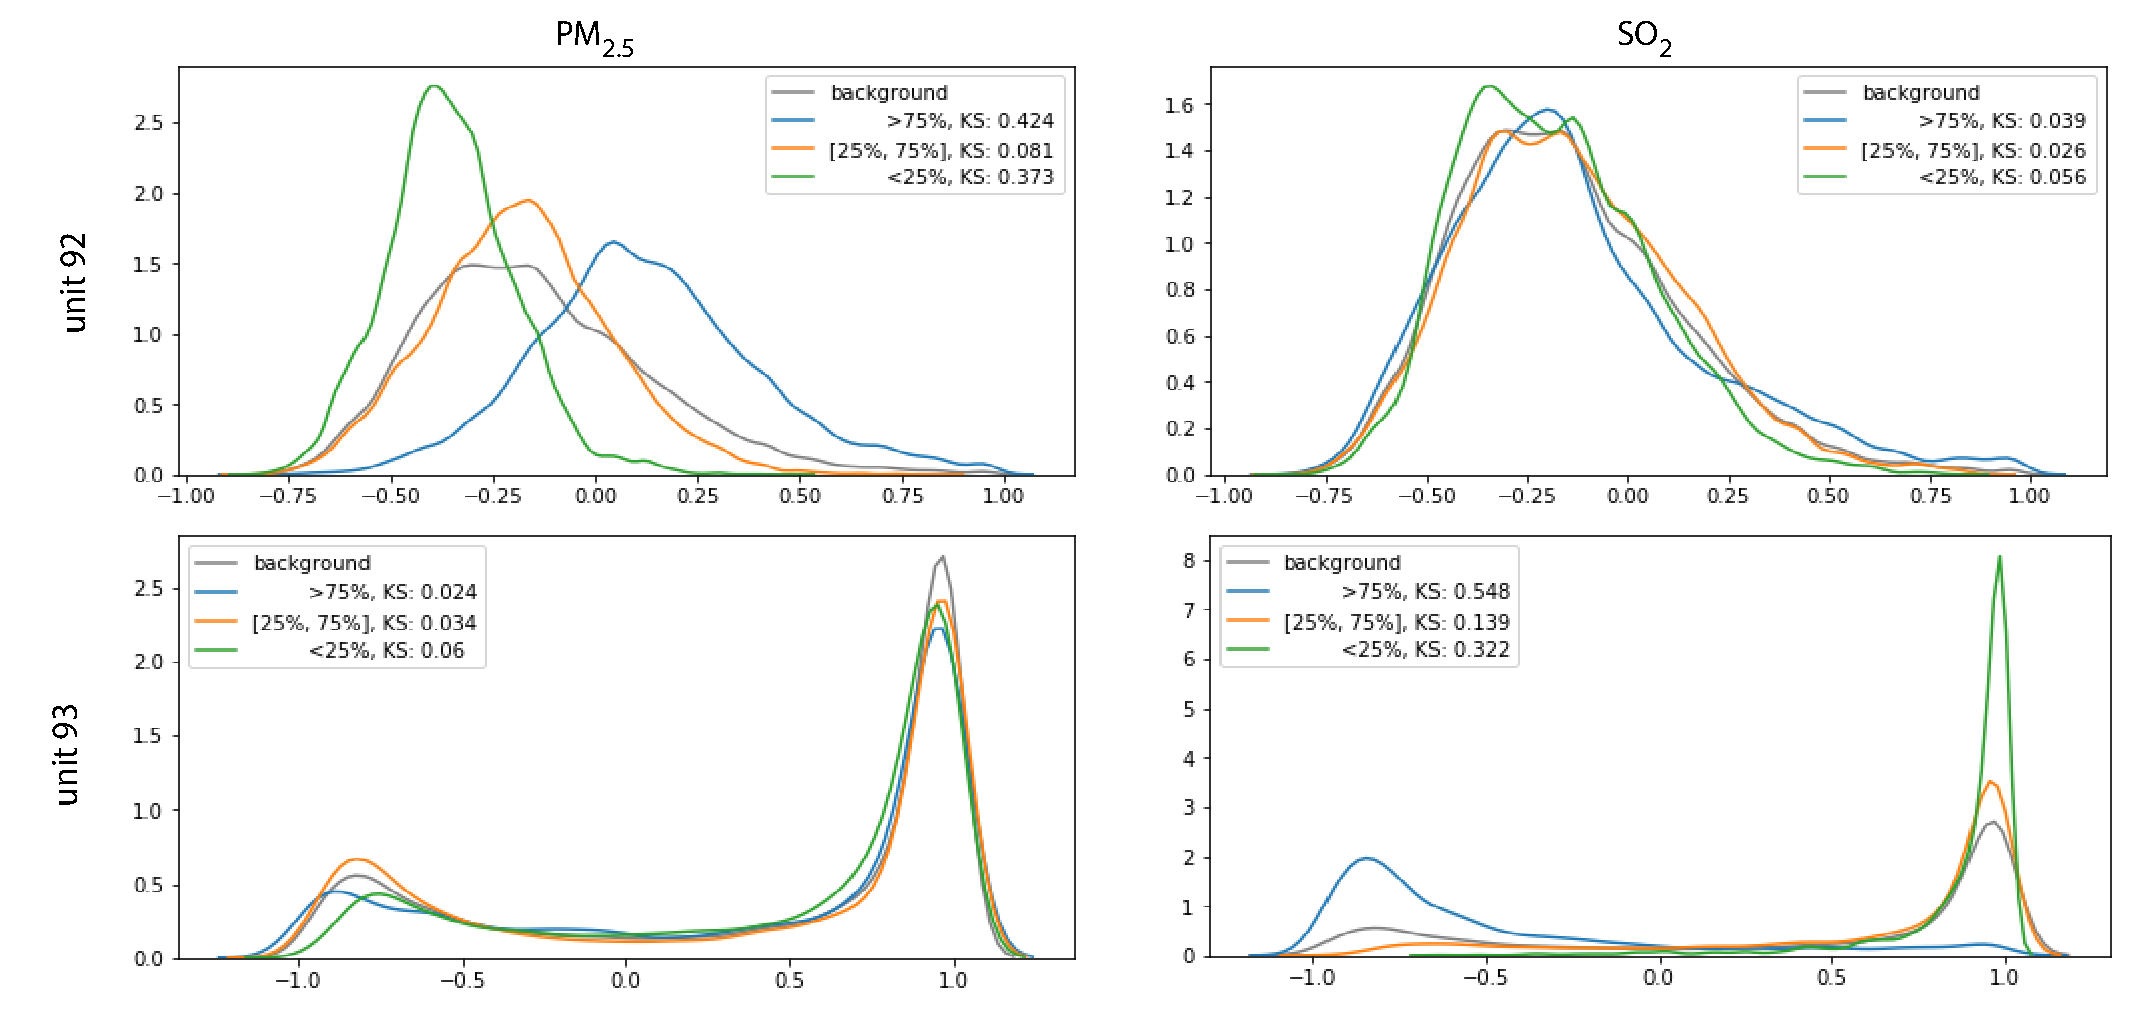
\includegraphics[width=0.95\textwidth]{figure/MultiRNNExplorer/methods/unit_response_kdeplot.pdf}
	\vspace{-3mm}
	\caption{Compare the response of hidden units(92 and 93) to features ($PM_{2.5}$ and $SO_2$). 
% 	Top left and bottom right: the distribution of the background is different from the distribution of other feature selections, which shows the hidden unit 92 and 93 response to $PM_{2.5}$ and $SO_2$ respectively.
	}
	\label{fig:unit_distribution_subgroup}
	\vspace{-1mm}
\end{figure}


To quantitatively measure the relationship strength between a hidden unit and a specific input feature, we compare the hidden unit distribution of data in different feature ranges with the distribution of all the data.
A larger difference indicates a stronger relationship as the hidden unit will generate different values when the feature value changes. As shown in Fig.~\ref{fig:unit_distribution_subgroup}, the ks-statistics of unit 92-$PM_{2.5}$ and unit 93-$SO_{2}$ are significantly larger than the other two combinations, indicating the statistics can effectively measure the distribution difference.
% Specifically, the relationship strength between the $j^{th}$ hidden unit and feature $f$ can be calculated as:
Specifically, the relationship strength between the $j^{th}$ hidden unit and feature $f$ can be measured as the maximum ks-statistics among all different feature selections:
\begin{equation}
    \label{equation:qualify_response}
    \begin{split}
    RS(j, f) = & max(Dis(\mathsf{H}^{j, f},~\mathsf{H}_{perc<0.25}^{j, f}), \\ 
    & Dis(\mathsf{H}^{j, f},~\mathsf{H}_{0.25~\leq~perc<0.75}^{j, f}), \\ 
    & Dis(\mathsf{H}^{j, f},~\mathsf{H}_{perc~\geq~0.75}^{j, f}))
    \end{split}
\end{equation}

\subsection{Hidden Unit and Feature Clustering} \label{section:clustering}
Another major challenge for interpreting RNN models on multi-dimensional sequential data is scalability.
RNN models usually contain hundreds to thousands of hidden units for each layer, which makes it ineffective to display the activation distribution of every hidden unit to users.
To address this challenge, previous work on visual interpretation of machine learning models usually use clustering~\cite{ming2017understanding, liu2017towards} or sampling~\cite{pezzotti2018deepeyes} techniques to reduce the number of visual elements displayed.
In this work, we choose clustering methods over sampling since clustering can better preserve the hidden units' response relationship to features. It also provides a good summary of the knowledge that the model learned. 

With the measurement of unit response, we can generate a 2D table with the size of $D \times\ M$, where $D$ and $M$ are the size of hidden units and features respectively. The cell of $j^{th}$ row and $k^{th}$ columns is the response of hidden unit $h^j$ to feature $f^k$: $RS(j,f^k)$. Then we can define the response embedding vector for both features and hidden units. For any feature $f^k$ and hidden unit $j$, the response embedding vectors are $vec_{f^k}= [RS(0, f^k), RS(1, f^k), ..., RS(D-1, r^k)]$ and $vec_{j}= [RS(j, f^0), RS(j, f^1), ..., RS(j, f^{M-1})]$, which are the specific columns and rows respectively. 

To analyze the relationship between hidden units and features, Yao et al.~\cite{ming2017understanding} used a bipartite graph to model the many-to-many relationship and used co-clustering algorithms~\cite{dhillon2001co} to group hidden units and input features simultaneously. We test co-cluster techniques: Spectral Co-clustering(SCoC) as well as other techniques including Agglomerative Clustering(AC) and Spectral Clustering(SC) on our dataset. The clustering methods other than SCoC take response embedding vectors as input to cluster features and hidden units respectively. To rank the performance of different clusters with different cluster numbers, we use the Silhouette Coefficient~\cite{rousseeuw1987silhouettes} to evaluate the quality of the clusters. Silhouette Coefficient ranges from -1 to +1,  with higher values of this coefficient meaning the cluster quality is more appropriate. 


Fig.~\ref{fig:cluster_parameters} shows cluster quality for features (left) and hidden units (right). We found that the Spectral Co-clustering method has a low Silhouette Coefficient score because it keeps creating a one-to-one relationship between the feature cluster and the hidden units cluster. In this case, it can be found that Agglomerative Clustering with cluster number of 12 and K-Means with cluster number of 10 show the best performance for feature and hidden units respectively.
With the Silhouette Coefficient, our system can automatically choose the clustering algorithms and cluster number.
Users can also manually choose different clustering algorithms and change the number of clusters based on their analysis requirement.



\begin{figure}[t]
	\centering
	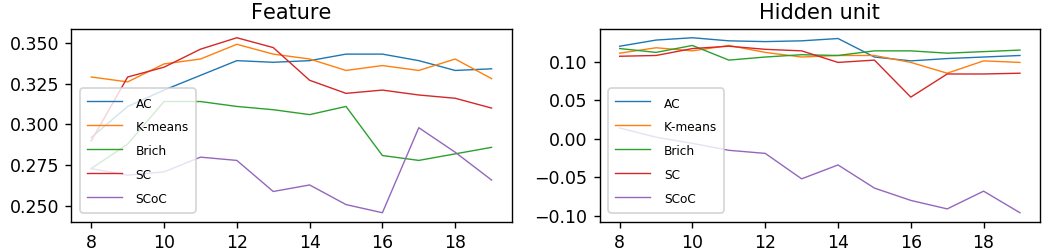
\includegraphics[width=0.95\textwidth]{figure/MultiRNNExplorer/methods/cluster_parameters.png}
	\vspace{-3mm}
	\caption{Cluster score with different cluster number. Left: feature cluster. Right: hidden unit cluster. The horizontal axis represents the cluster number, the vertical axis represents the cluster score. 
% 	A good choice of the cluster method and cluster number is K-means and 12 for the feature cluster, Agglomerative Clustering (AC) and 10 for the hidden units cluster.
	}
	\label{fig:cluster_parameters}
	\vspace{-1mm}
\end{figure}

The clustering results can be modeled as bipartite graph $\mathbb{G} = (\mathbb{V}_H, \mathbb{V}_F, \mathbb{E})$, where $\mathbb{V}_H$ is the hidden unit cluster set and $\mathbb{V}_F$ is the feature cluster set. $\mathbb{E}$ indicates the weighted edge set between unit clusters and input dimension clusters with the weight of $E_{H,F} = \displaystyle\sum_{h \in H}\displaystyle\sum_{f \in F}RS(h, f)$ where $H \in \mathbb{V}_H$ and $F \in \mathbb{V}_F$. 

This bipartite graph of features and hidden units can help users understand the information captured by different hidden unit clusters by examining which feature clusters have strong relationships with them.



\subsection{Local Feature Importance}\label{section:feature_importance}

Inspired by back-propagation in machine learning, we conduct the individual level analysis based on the local gradient which is used to present the word saliency in NLP tasks~\cite{li2015visualizing}. 
Given the output of feature $y^l$, we use the local gradient with respect to feature $x_t^k \in x$ to present the feature importance as:

\vspace{-3mm}
\begin{equation}
    \label{equation:feature_gradient}
    \begin{multlined}
    w(y^l, x_t^k) = |\frac{\partial(y^l)}{\partial(x_t^k)}|
    \end{multlined}
\end{equation}


The absolute value of gradient $w(y^l, x_t^k)$ indicates the sensitiveness of $x_t^k$ to the final decision of  $y^l$ with the given input sequence of $x$. This measurement shows how much the specific feature at a specific time contributes to the final output~\cite{li2015visualizing}.
However, for input $x$ with the length of $T$,  the total number of all feature importance scores is $N \times T$ which causes difficulty in showing the overview. To address this challenge, we leverage the clustering result from Sec.\ref{section:clustering} and define the cluster importance of features as:
\begin{equation}
    \label{equation:cluster_gradient}
    \begin{multlined}
    W(y^l, H^i_t) =\displaystyle\sum_{x^k_t \in H^i_t}|w(y^l, x^k_t)|
 \end{multlined}
\end{equation}
\QM{Thus, the size of the cluster importance for all timestamps is $C \times T$ where $C$ is the number of clusters ($C<N$)}. 

\section{Visualization Design}


In this section, we introduce the visual design based on the design tasks discussed in Sec.\ref{section:design_tasks}.  As shown in Fig.~\ref{fig:teaser}, the visual analytic system consists of six coordinated views. Starting from the configuration panel Fig.~\ref{fig:teaser}B, the users are able to select the target feature and the model to be analyzed. The region partition will be shown as Fig.~\ref{fig:teaser}B after the model is selected. To support exploring the model mechanism, the Cluster View is displayed to summarize the hidden units' response to the features (Fig.~\ref{fig:teaser}A) and the Feature Importance View (Fig.~\ref{fig:teaser}C) is shown to visualize the temporal importance of each feature. Furthermore, the users can select the individual cases in the Projection View (Fig.~\ref{fig:teaser}E) and all the selected individual cases are grouped by similarity and displayed in the Individual View (Fig.~\ref{fig:teaser}D).


\begin{figure}[t]
	\centering
	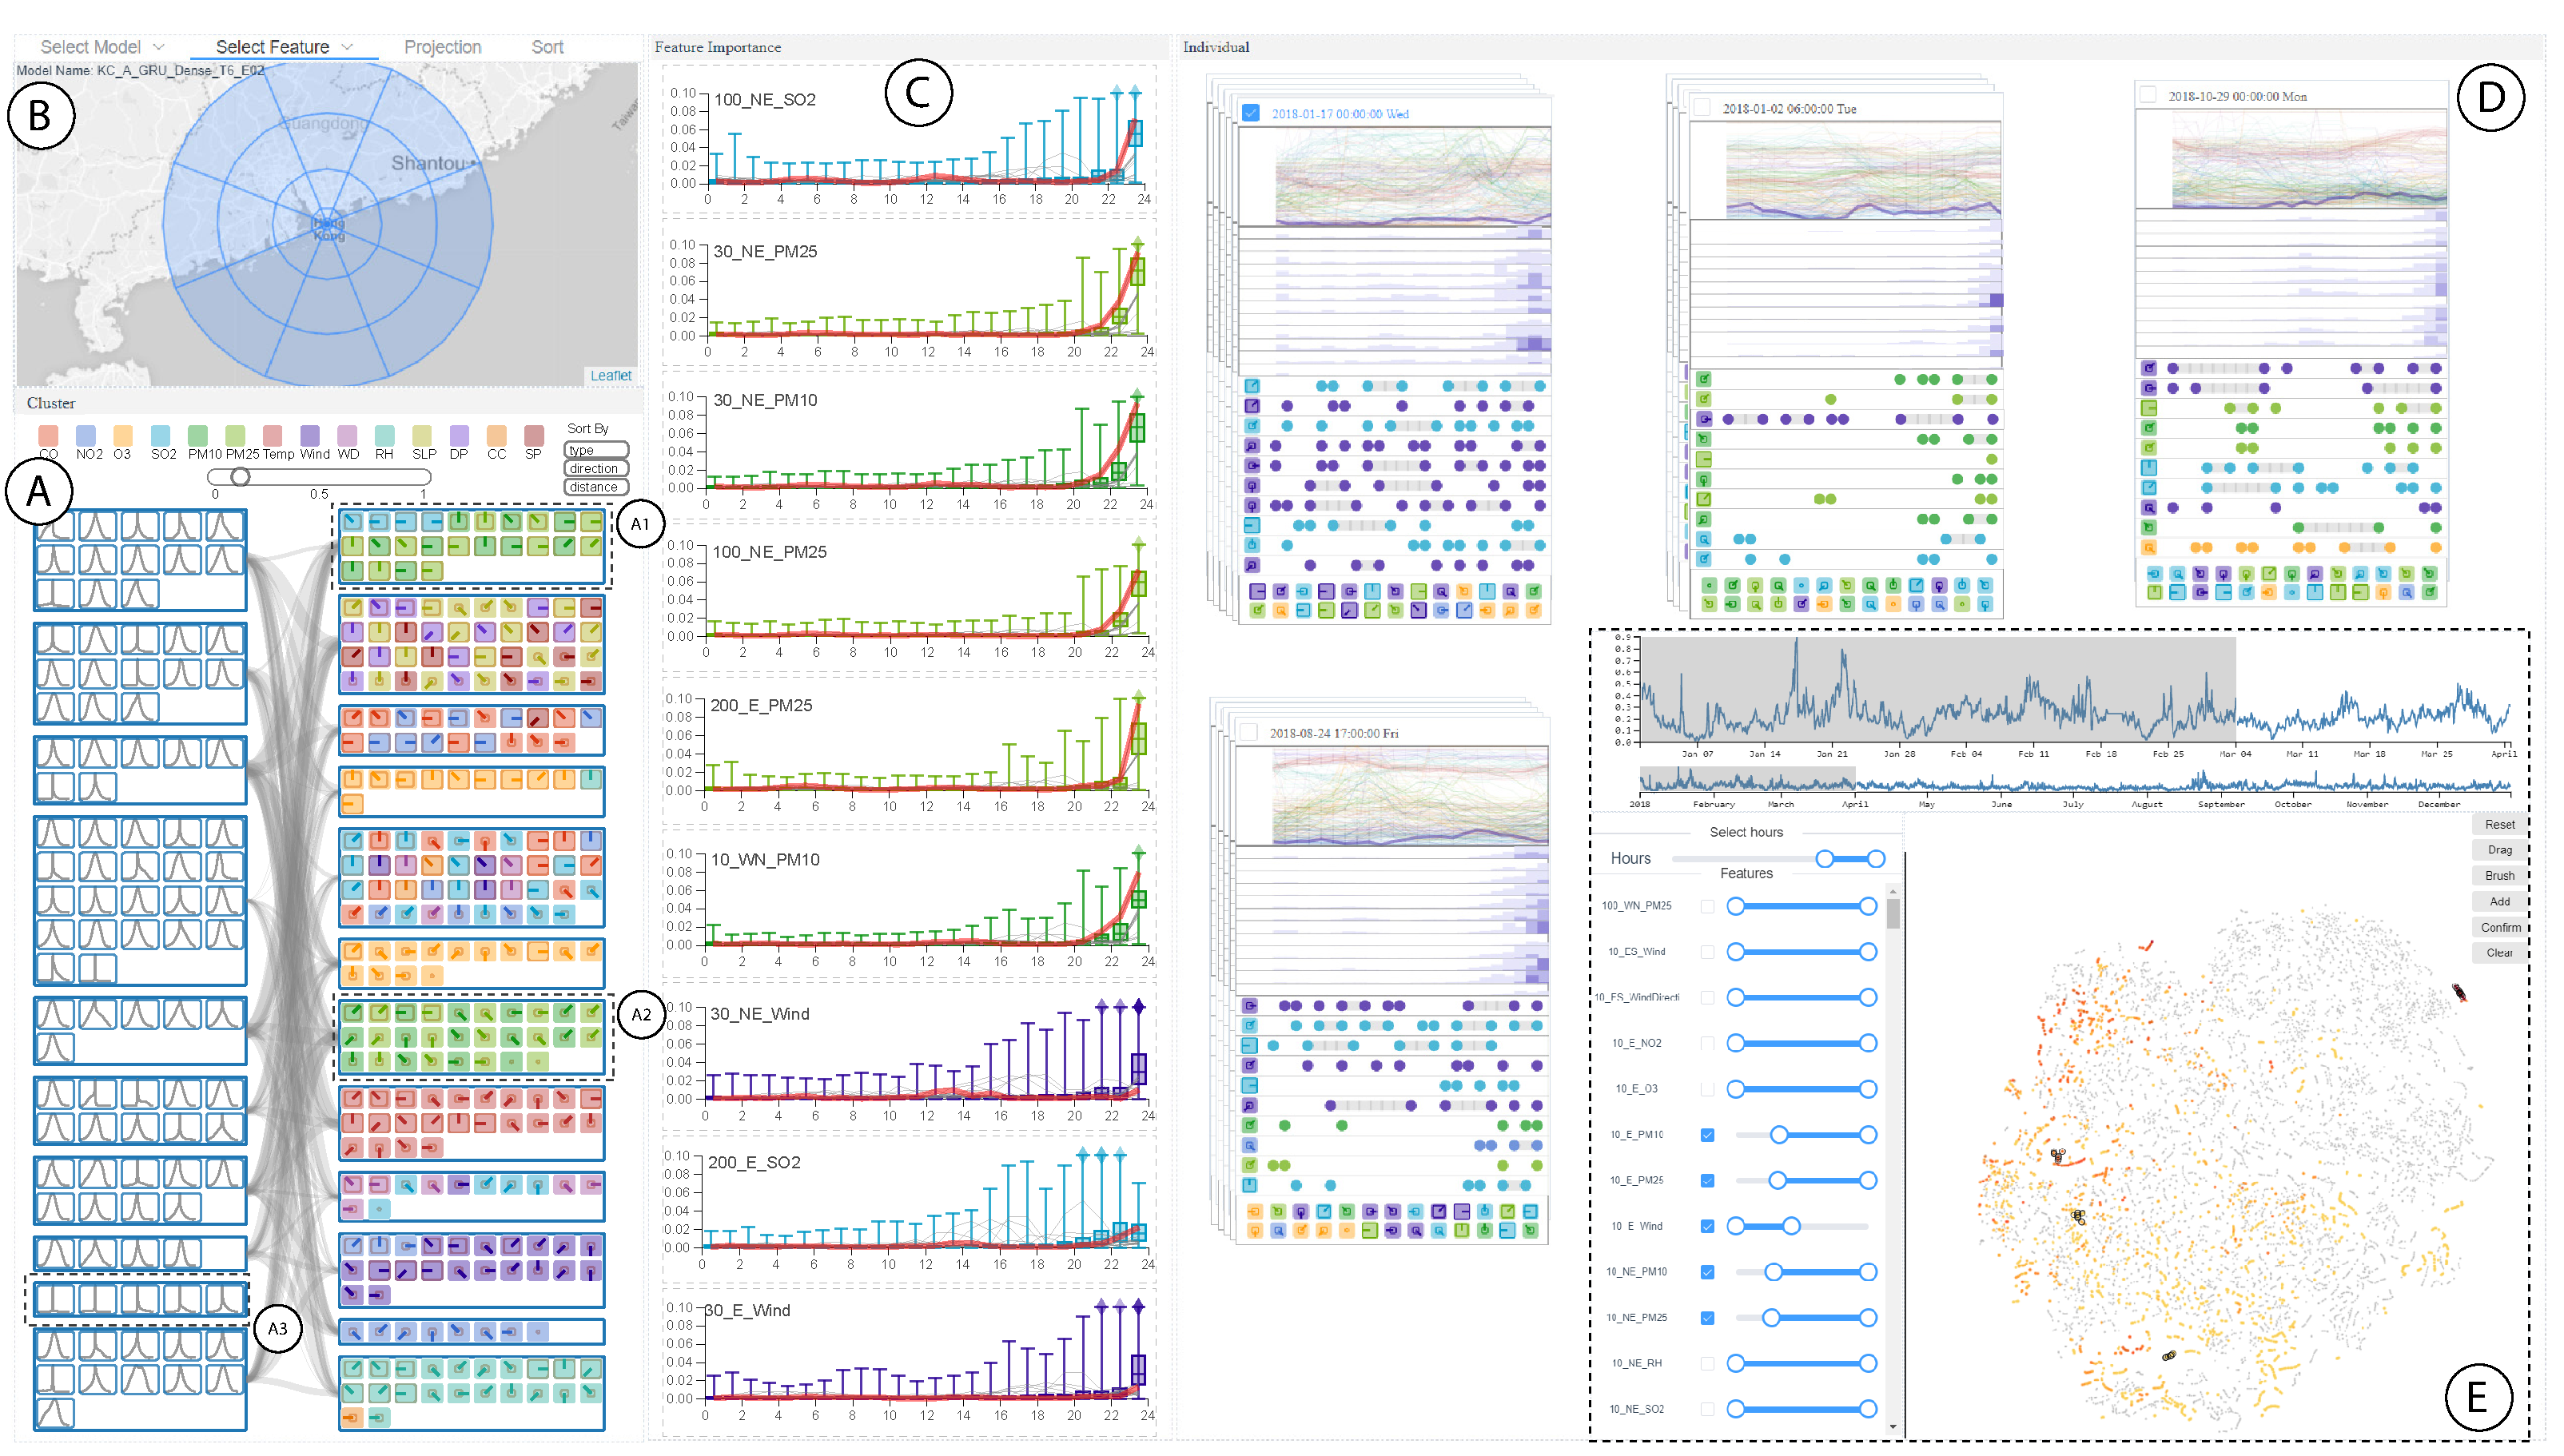
\includegraphics[width=0.95\textwidth]{figure/MultiRNNExplorer/teaser.pdf}
	\vspace{-3mm}
	\caption{Design of Hidden unit distribution and feature glyph. A) Hidden unit cluster; B) Hidden unit distribution; C) Feature cluster; D) Feature distribution for selected features; E) Feature glyph design; G) Response link MultiRNNExplorer contains multiple coordinated views to support exploring and understanding RNNs' behaviors on multi-dimensional time-series data, especially on hidden unit response and feature importance.
		The Configuration Panel (B) allows users to select a RNN models and configure parameters. 
		To reveal model mechanism, the Cluster View (A) summarizes the hidden unit clusters' response to feature clusters, and the Feature Importance View (C) summarizes the temporal importance of input features. 
		The Projection View (E) displays a data overview, allowing users to identify and select sequence instances of interest for further analysis. 
		The selected instances will be shown by the Individual View (D). }
	\label{fig:teaser}
	\vspace{-1mm}
\end{figure}
%!TEX root = ../article.tex
\subsection{Cluster View}
% To enable users to observe the statistics of both the features and hidden states (\textbf{T1},\textbf{T2}), we develop the Cluster View (Fig.~\ref{fig:teaser}).
% It shows the overview of response relationship (\textbf{T3}) between the hidden units and features. The hidden units and features are visualized as the Hidden State Distribution and the Feature Glyph respectively.

The Cluster View (Fig.~\ref{fig:teaser}A) shows the overview of response relationship (\textbf{T3}) between the hidden units and features. The hidden units and features are visualized as the Hidden State Distribution and the Feature Glyph respectively.


\begin{figure}[t]
	\centering
    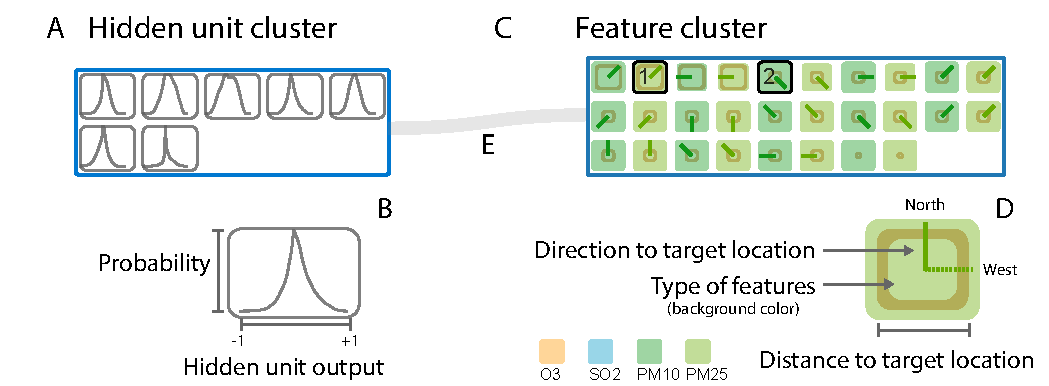
\includegraphics[width=0.95\textwidth]{figure/MultiRNNExplorer/design/cluster_design.pdf}
	\vspace{-3mm}
	\caption{Design of Hidden unit distribution and feature glyph. A) Hidden unit cluster; B) Hidden unit distribution; C) Feature cluster; D) Feature distribution for selected features; E) Feature glyph design; G) Response link}
	\label{fig:cluster_design}
	\vspace{-1mm}
\end{figure}


\textbf{Hidden State Distribution.}
The left column on the Cluster View is the Hidden State Distribution component.
As shown in Fig.~\ref{fig:cluster_design}A, each row represents a hidden unit cluster.
% The row height increases with the number of hidden states in each cluster.
Each hidden unit in a cluster is represented as a line chart that shows its activation distribution(\textbf{T1}).
The x-axis represents the hidden unit output ranging from $-1$ to $+1$ and the y-axis represents the \UC{corresponding probability} (Fig.~\ref{fig:cluster_design}B).
From the line chart, users can observe and compare the activation distribution patterns of different hidden units. 

\textbf{Feature Glyph.}
The right column of the Cluster View is the Feature Glyph component (Fig.~\ref{fig:cluster_design}C).
Similar to the Hidden State Distribution, each row represents a feature cluster in which a glyph (Fig.~\ref{fig:cluster_design}D) represents a feature.
As described in Sec.~\ref{section:application}, we define our usage scenario as air pollution forecasting.
Each feature has three identifiers: the feature category, the direction, and the distance from the feature to the target location.
The background color of the feature glyph cell encodes the feature category.
We use a categorical color scheme to encode different categories, and users can find the color legend at the top of the Cluster View.
\UC{In each feature glyph, the distance and direction to the target location are presented by a rectangle and a line segment with one end point at the center.}
The angle of the direction bar encodes the direction, and the width of the distance rectangle represents the distance(Fig.~\ref{fig:cluster_design}D).

\textbf{Interactions.}
We also support various interactions to allow users to dynamically explore this view.
The curves linking the hidden state cluster and feature cluster with the width indicate the response strength (Fig.~\ref{fig:cluster_design}E). Users can also filter the link according to the response strength by adjusting the slider bar. 
When hovering over a hidden state cluster or a feature cluster, the corresponding links and linked clusters will be highlighted.

In this view, the users can obtain an overview of the response relationship between hidden units and features, for example, we can find that there are not strong links connecting to cluster 8 (Fig.~\ref{fig:teaser} A$_3$), this may be because that all the hidden units are ``weakly'' activated in cluster 8.
% Users can also select a feature for further examination by clicking the corresponding feature cell.
% After clicking, a line chart will be appended to the right of the Feature Distribution component (Fig.~\ref{fig:cluster_design}D) to show the feature's value distribution.

\subsection{Feature Importance View}
The feature importance view allows users to explore the feature contribution to model output (\textbf{T2}).
As discussed in Sec.\ref{section:feature_importance}, with an input case, we are able to measure the importance of a single feature as a sequence of importance scores which correspond to the importance at all timestamps (Fig.~\ref{fig:teaser}C). 

Since the importance score only provides a local description for the feature importance, an effective visualization is needed to show an overview of each feature's importance. We choose boxplot for this task since it can present the statistics overview. To show the temporal trend of a feature, we group the importance score of all test cases by the timestamps and make statistics group by group. For the test sequence with a length $T$, will use the feature importance charts which contain $T$ boxplots to show the trend of feature importance (Fig.~\ref{fig:teaser}C).

The horizontal axis indicates the timestamps and the vertical axis indicates the feature importance score. The top line, upper edge, middle line, bottom edge and bottom line of the boxplot indicate the maximum,  $75^{th}$ percentile, mean, $25^{th}$ percentile and minimum of the importance scores.  Since sometimes the maximum will much larger than the $75^{th}$  percentile value, which makes the box vary flat and difficult for users to explore the temporal pattern, we limit the maximum score $Ms$ shown in the view. If a boxplot has scores larger than $Ms$, a diamond symbol appears on the top of the boxplot. The opacity of the diamond indicates the magnitude of the absolute difference between the largest score and $Ms$.    

We also define the overall importance score for a single feature as the sum of the mean score at all timestamps. By default, the boxplot charts will be ranked according to the overall feature importance score. Due to the large number of features, only the top 10 feature importance charts are visualized. Users may observe other features by using the scroll bar or filtering the features from the projection view (Fig.~\ref{fig:teaser}C). 


%!TEX root = ../article.tex
\subsection{Projection View}
To help users obtain an overview of case clusters and outliers (\textbf{T5}), we design the Projection View (Fig.~\ref{fig:teaser}E) which supports various interactions such as zooming and brushing to allow users to select a subset of data for further examination.

In the Projection View, each circle represents a individual case. There are many multi-dimensional reduction methods such as MDS and PCA; we select t-SNE as it can strongly repel dissimilar points and show clusters clearly.
For each case, we collect the feature cluster importance over all time steps (discussed in Sec.\ref{section:feature_importance}) as the input vectors of t-SNE.
% \QM{Given an individual case, we flatten the cluster importance at all timestamps (discussed in Sec.\ref{section:feature_importance}) to 1-dimensional as the t-SNE embedding vector.}
% \yh{?}
Thus, the positions of the circles reflect the similarity of their cluster importance.

% Add to increase the space
% When multiple data subsets are selected, we use a categorical color scheme to fill the circles so that the data sequences from the same data subset will have the same color in both components.
% Users can brush to select data sequences for detailed examination in the Sequence View.

% One major consideration in developing the Projection View is the scalability problem.
% When the number of circles is large, the circles may overlap with each other, and the Projection View can be cluttered.
% We adopt a node overlap removal algorithm for the similarity projection and support panning and zooming to allow users to explore a data subset.

Furthermore, to improve the flexibility of the case selection, we add a two-scale timeline (Fig.~\ref{fig:teaser}E top) to show the target feature trend, enabling user filtering of the cases by time, and a feature selection component (Fig.~\ref{fig:teaser}E left) to filter the cases by feature value.  


%!TEX root = ../article.tex
\subsection{Individual View}
After observing an overview on data similarities, users may need to drill down to a few individual cases of interest for detailed examination.
We develop the Individual View for users to explore and compare the different individuals over time (\textbf{T6}).
% Specifically, our goal is to identify the important features at different time steps and their relationship to raw feature values (\textbf{T2}, \textbf{T4}).


\begin{figure}[t]
	\centering
    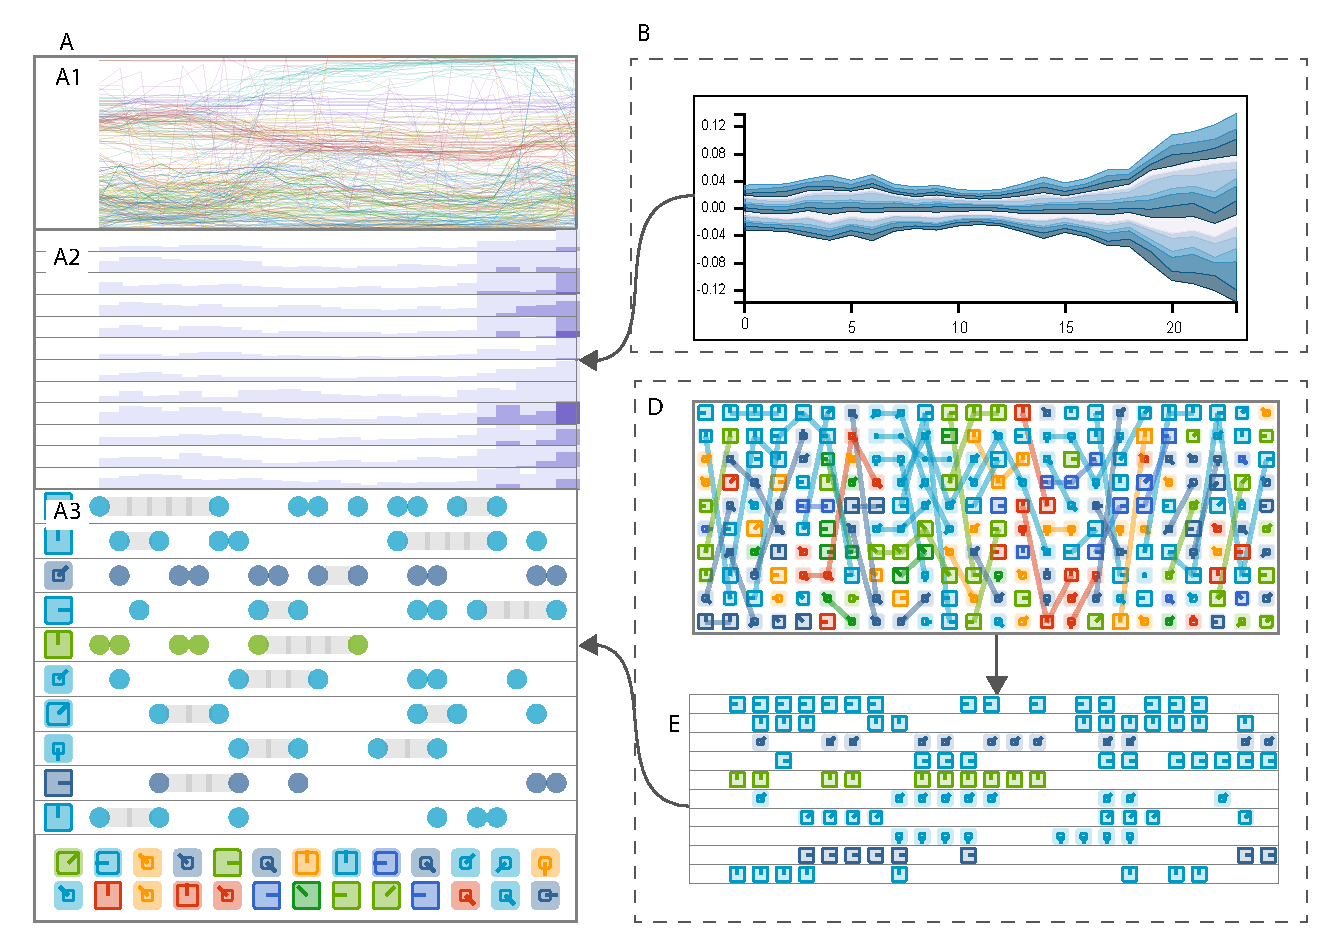
\includegraphics[width=0.90\textwidth]{figure/MultiRNNExplorer/design/alternative_design.pdf}
	\vspace{-3mm}
	\caption{Individual design and the alternative designs. A) Individual View. A1) Feature Trend Chart; A2) Cluster Importance Chart; A3) Top Features Chart. B) themeriver as the alternative design of the Cluster Importance Chart; C) and D) node-like sequence and node sequence as the alternative design of Top Features List.}
	\label{fig:individual_view}
	\vspace{-1mm}
\end{figure}

% cell -> card
\UC{The selected individual cases are visualized as several stacks of \UC{cell} as in Fig.~\ref{fig:individual_view}A.
Each cell consists of three components: the Feature Trend Chart (Fig.~\ref{fig:individual_view}A$_1$), the Cluster Importance Chart (Fig.~\ref{fig:individual_view}A$_2$), and the Top Feature List (Fig.~\ref{fig:individual_view}A$_3$).
All these three components share the same x-axis which represents the time where time steps increase from left to right.}

Feature Trend Chart is a multi-line chart that depicts how different features' values change over time. 
The y-axis represents normalized feature values where the feature value increases from bottom to top ranging between 0 and 1.
Each line represents a feature and the line color encodes feature category the same as in the Cluster View.
The corresponding lines are highlighted when hovering on any feature glyph in the Cluster View or hovering on feature importance view. 
% to enable users to focus on the features in the current context and avoid visual clutter.

The middle component is the Cluster Importance Chart, which is a list of horizon bar charts that summarize how each feature group's gradient changes over time.
Each feature group is represented as a \UC{horizon bar chart} and aligned vertically in the same order as the Cluster View.
For a horizon bar chart, each bar represents the averaged gradient for the corresponding feature group at one time step. 
We use both the bar height and bar color to encode the gradient value.
As shown in  Fig.\ref{fig:individual_view}A$_3$, the first visual channel to encode gradient value is bar height where a greater height indicates a larger gradient value.
When the gradient value exceeds a certain limit, we clip the bar and overlay another darker bar with the same height as the clipped part at the same position for better vertical space efficiency.
We have also considered other design choices such as a themeriver (Fig.\ref{fig:individual_view}B) in which each colored flow indicates a feature group. 
However, comparing different feature groups may be difficult and it requires more space when the gradient is large.
Thus, we abandon this alternative choice and adopt the current design.

\UC{
Though the Cluster Importance Chart provides an overview of how each feature cluster's importance changes over time, users still need to link this component to the Cluster View to observe which features are considered important by the model.
We design a Top Feature List to visualize the important features over time. 
Our first design is shown in Fig.~\ref{fig:individual_view}D. where the top $N$ features ranked by importance are visualized as feature glyphs at each timestamp. 
We draw links to connect glyphs that represent the same feature in consecutive time steps.
However, this design leads to serious visual clutter due to link overlap when feature ranks are frequently changed over time. 
To alleviate users' mental burden, we develop a new design as shown in Fig.~\ref{fig:individual_view}E.
% We visualize the top $N$ features that have the largest average gradients over time. 
Each feature is represented as a row and we draw its corresponding feature glyph at the timestamps when this feature is ranked in the top $N$ most important features. 
To simplify this visual design, we position the feature glyph at the beginning of each row. 
% As a feature has different gradients over time, the importance ranking of a feature can also vary at different steps.
We then use two colored circles linked with gray lines to indicate at which time steps the corresponding feature is ranked in the top $N$ mostly important features.
The circle color is consistent with the feature glyph color.
To make the Top Feature List space efficient, we only show ten rows by default, and other features are collapsed as feature glyph rows as shown in the bottom at Fig.\ref{fig:individual_view}A$_3$.
Users can click the glyph rows to select different features to analyze.
}

\UC{The three components enable users to observe which features are considered important by the model over time and how the importance is related to feature value changes.
Users can also append multiple cells to the Sequence View to compare different sequences side by side. 
When the number of cells becomes large, we use dbscan to cluster the similar individual cases by the fatten cluster importance(discussed in sec. \ref{section:feature_importance}) into one stacked cells with one randomly selected case as the representative case at the top of stack.}

\subsection{Interactions and Linkage}
To better facilitate the interactive exploration of RNNs, our system supports cross-view interactions. 
% In this section, we summarize the interactions and linkage among all four views.

\textbf{Cross-view highlight.} 
There are three key visualization components appearing across different views: \textbf{features}, \textbf{feature clusters}, and \textbf{cases}. 
These components are visualized and encoded in different approaches in across views to support various analysis requirements. 
% For example, a feature is visualized as a glyph (Fig.\ref{fig:cluster_design}E) in the cluster view,  visualized as a series of boxplots (Fig.\ref{fig:teaser}C) in the Feature Importance View and shown as both a line chart (Fig.\ref{fig:individual_view}A$_1$) and a sequence (Fig.\ref{fig:individual_view}A$_3$) in the individual view. 
If one feature is selected, its corresponding visual elements in other views will be highlighted.

% In summary, there are three key visualization components appearing across different views: \textbf{feature}, \textbf{feature cluster} and \textbf{case}. These components are visualized in different forms in different views to support various analysis requirements. For example, a feature is visualized as a glyph (Fig.\ref{fig:cluster_design}E) in the cluster view,  visualized as a series of boxplots (Fig.\ref{fig:teaser}C) in the Feature Importance View and shown as both a line chart (Fig.\ref{fig:individual_view}A$_1$) and a sequence (Fig.\ref{fig:individual_view}A$_3$) in the individual view. If one feature is selected by mouse hover, the corresponding visualization element in other views will be highlighted with a border stroke.

\textbf{Linkage between individual view and feature importance view.} 
When multiple individual cases are selected, the feature importance by time will be visualized as multi-line charts as Fig.~\ref{fig:teaser}C shows. 
When users hovering over an individual case , the corresponding line-chart will be highlighted. 
% If the user selects multiple individual cases using check boxes, the corresponding line charts will be highlighted in red color.


% \textbf{Linkage between individual view and feature importance view.} 
% When multiple individual cases are selected, in addition to visualizing these cases in individual views, the feature importance by time will be visualized as a line chart in the corresponding feature importance views as Fig.\ref{fig:teaser}C shows. When the user chooses an individual case by mouse hover, the corresponding line-chart will be highlighted by border stroke width. If the user selects multiple individual cases using check boxes, the corresponding line charts will be highlighted in red color.


\section{Case study}
% \yh{We may 1) change terms like the epoch 5, 40 to the $5^{th}$, $40^{th}$ epoch; and 2) Capitalize the first letter of each word in view names such as cluster view to the Cluster View.}

In this section, we demonstrate the effectiveness of MultiRNNExplorer in analyzing model behaviors and feature importance. 
We use the air pollutant data between 2015 to 2017 to train the model and use 8,375 cases in 2018 as testing data for analysis. 
% Notice that feature importance and hidden unit response are calculated on testing data,  
% The testing dataset contains the 8,375 individual cases in the year 2018.
The accuracy and hyper-parameters of different models are listed in Table~\ref{table:model_configuration}. 
We demonstrate our system to the domain expert and analyze the trained models on several tasks.

\begin{table}[h!]
\centering

\begin{tabular}{|p{3cm}|p{1cm}|p{3cm}|p{3cm}|} 
 \hline
 Model & Size & Dense Layer & MSE ($PM_{2.5}$) \\ [0.5ex] 
 \hline \hline
    Vanilla RNN&100&No&5.31 $\pm$ 0.98 \\
    GRU&100&No&4.32 $\pm$ 0.51\\
    LSTM&100&No&4.81 $\pm$ 0.31\\
    GRU-Dense&100&3&4.25 $\pm$ 0.21\\
    LSTM-Dense&100&3&4.53 $\pm$ 0.53\\
\hline
\end{tabular}
\caption{Configuration and performance of RNNs, including vanilla RNN, GRU, LSTM, and the RNNs with dense layer (e.g., RNN-Dense). The performance is evaluated by the mean square error (MSE) of $PM_{2.5}$; low MSE represents better performance.}
\label{table:model_configuration}
\vspace{-8mm}
\end{table}


\subsection{Changes Over Epochs}
To explore the model behavior over the training process, we manually select the RNN model trained after 5, 40, 120, and 200 epochs. Fig.~\ref{fig:evolution_epochs} shows the projections and top five most important features at different epochs.

In the Projection View (Fig.~\ref{fig:evolution_epochs}A), we choose $PM_{2.5}$ as the target feature and use a sequential color schema to indicate the predicted value where a darker color indicates a higher $PM_{2.5}$. 
At early stages ($5^{th}$ and $40^{th}$ epochs), we find that the points in a darker color are distributed uniformly in the projection and are mixed together with the points with a light color. 
This indicates that the cluster gradients are not able to present the distribution of the target feature yet.
After training more epochs, the dark points become more concentrated. 

In addition, the Feature Importance View (Fig.~\ref{fig:evolution_epochs}B) shows that the magnitude of the gradient starts from a small value and then keeps increasing in the training process. 
We also find that in the $5^{th}$ and $40^{th}$ epochs, the top five important features are $\color{PM25Color}{PM_{2.5}}$ and $\color{PM10Color}{PM_{10}}$ while in the $120^{th}$ epoch, the feature of wind speed is also ranked in the top five most important features. 
In the $200^{th}$ epoch, more features related to wind speed are listed in the top five features.
Another finding is that in the $5^{th}$ epoch, we observe that only the features from the last time steps are considered important while the models at the $40^{th}$, $120^{th}$, and $200^{th}$ epochs leverage more timestamps in the forecast.  
The domain experts indicate that the $PM_{2.5}$ and $PM_{10}$ at nearby locations are the most intuitive features to forecast $PM_{2.5}$ ($PM_{10}$ and $PM_{2.5}$ are always highly correlated).
Moreover, the last time step is very important because it is the closest one to the final prediction. 
Based on these observations, we infer that the features that are directly related with the targeted air pollutant are considered important in the early stage of the training process.
After more epochs, the model starts to learn other features that may indirectly influence the forecast, such as the \textit{\color{WINDColor}{Wind Speed}} and other pollutants ($\color{SO2Color}{SO_2}$ or $\color{NO2Color}{NO_2}$) (shown as Fig.~\ref{fig:evolution_epochs}B, 20$^{th}$,200$^{th}$ epochs). 

\UC{According to official website of United States Environmental Protection Agency (EPA): ``$SO_x$ can react with other compounds in the atmosphere to form small particles. These particles contribute to particulate matter (PM) pollution"\cite{SO2TOPM25}.
We also discussed the reason that $SO_2$ becomes important later in training with the domain experts. 
They said it is also possible that the $SO_2$ relates some industrial activity which results in the high-air pollutant. }
% They explained that the sulfur oxides ($SO_x$) react with other compounds in the air and form tiny particles which contribute to the particulate matter. 
% A "Report on the Environment" from the EPA (United States Environmental Protection Agency) indicates that ``SO2 emissions are an important environmental issue because they are a major precursor to ambient $PM_{2.5}$ concentrations"\cite{SO2TOPM25}.
Moreover, the domain experts explain that the wind speed is important for several reasons: 1) the air pollutants will  be blown away if the wind speed is high; 2) since the north and west of the target location have more factories which are the major source of air pollutants, the appropriate wind speed and direction will bring the air pollutants to Hong Kong.
Moreover, the data also show different patterns in the Cluster View during the training process. 
For example, as shown in Fig.~\ref{fig:evolution_epochs}B, we found that in the $5^{th}$ epoch almost all three types of features: \textit{\color{SLPColor}{Sealevel Pressure}}, \textit{\color{DPColor}{Dew-point}} and  \textit{\color{SPColor}{Station Pressure}} are grouped into one cluster. 
After the $40^{th}$ epoch, we notice that this cluster is split into two clusters.
With these observations, we derive the conclusion that the model gradually learns the high-level knowledge in the training process.

\begin{figure}[t]
	\centering
	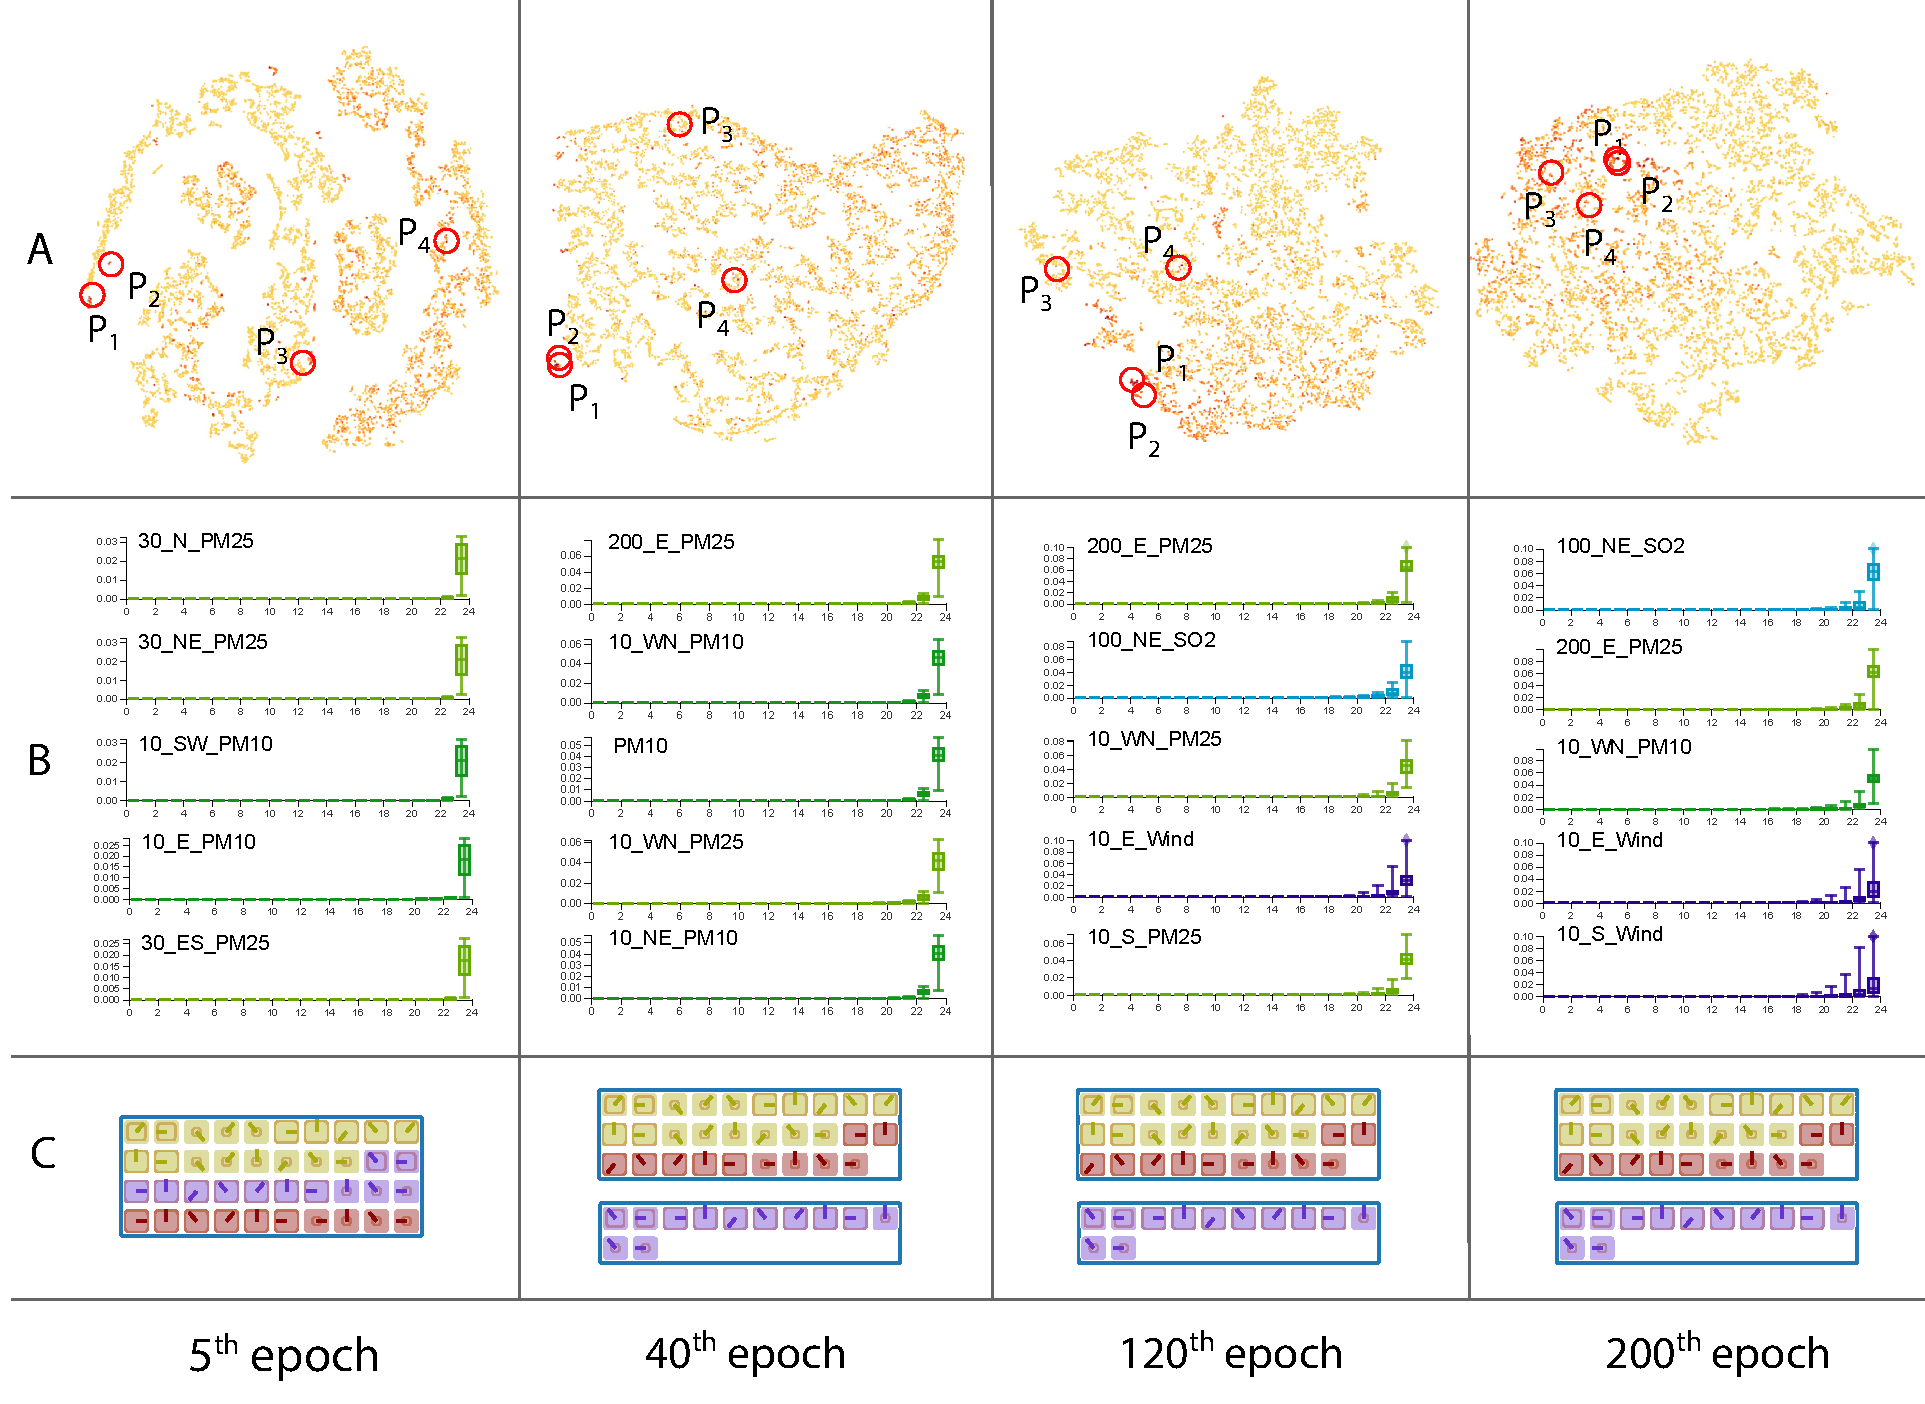
\includegraphics[width=0.45\textwidth]{figure/MultiRNNExplorer/Evaluation/evolution_epochs.pdf}
	\vspace{-3mm}
	\caption{\UC{The RNN model shows different behaviors along the training process. A, B, and C show the Projection View, top five important features, and feature clusters respectively at different epochs.}
% 	A: Projection Views shows the high-pollutant points gradually gathered during the training process; B: the top five important features at the corresponding epochs; C: the feature cluster change at each epoch.
	}
	\label{fig:evolution_epochs}
	\vspace{-4mm}
\end{figure}



\subsection{Understand Model Behaviors}
\begin{figure}[t]
	\centering
	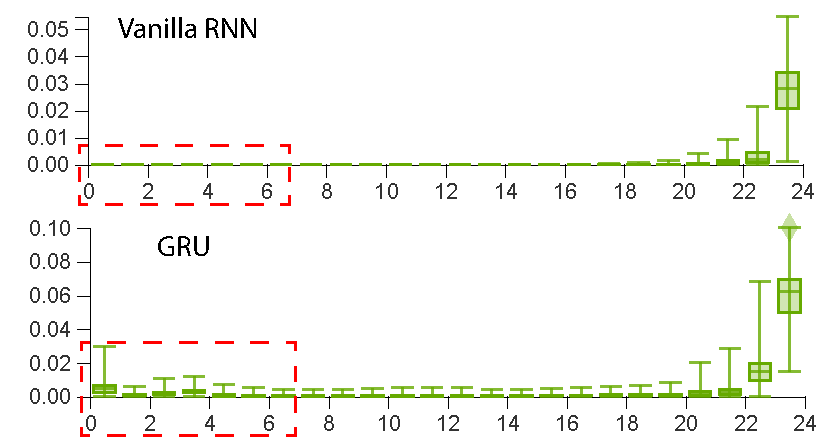
\includegraphics[width=0.40\textwidth]{figure/MultiRNNExplorer/Evaluation/FI_comparison.pdf}
	\vspace{-3mm}
	\caption{Compare the temporal importance of \textit{100\_NE\_PM25}  across different models. 
% 	The dashed rectangle show both GRU has a "tail" while vanilla RNN does not.
	}
	\label{fig:gru_vs_rnn}
	\vspace{-4mm}
\end{figure}

\subsubsection{Model Mechanism}
This case study is conducted to understand what RNN models learn and to compare different models trained for air pollutant forecasting. 
With MultiRNNExplorer, we are able to select models at any epoch. Fig.~\ref{fig:teaser}A shows the Cluster View of GRU-Dense; by observing the cluster of features, we find that the features with same feature types are likely to cluster together such as the \textit{\color{RHColor}{Relative Humidity}} and \textit{\color{DPColor}{Dew-point}}, are exactly grouped into two separated clusters shown as Fig.~\ref{fig:teaser}A$_4$.
Moreover, we find that the $\color{PM25Color}{PM_{2.5}}$ and $\color{PM10Color}{PM_{10}}$ are always clustered together as shown in Fig.~\ref{fig:teaser}A$_1$ and Fig.~\ref{fig:teaser}A$_2$.
The domain expert explains that $\color{PM25Color}{PM_{2.5}}$ and $\color{PM10Color}{PM_{10}}$ are highly correlated because they are always generated together.
% On the other hand, we notice that all the features on \color{PM25Color}{$PM_{2.5}$} and \color{PM10Color}{$PM_{10}$} are also grouped by the distance: Fig. \ref{fig:teaser}A$_1$ and A$_2$ show that the features far away from (200km and 300km) or nearby (closer than 30km) the target location are clustered in different groups. 
This  shows that the model GRU-Dense is able to learn the information related to spatial locations.  

% Another thing of interest is the hyper-parameters of the model such as the RNN size. 
% \yh{How the hidden unit size relates with the observation below?}
% In the cluster view, we notice that a cluster of hidden units have very weak relationship to feature clustersi(Fig. \ref{fig:teaser} a4. \QM{explain?}.
% Such pattern also appears in the exploration of other models.

\begin{figure}[t]
	\centering
	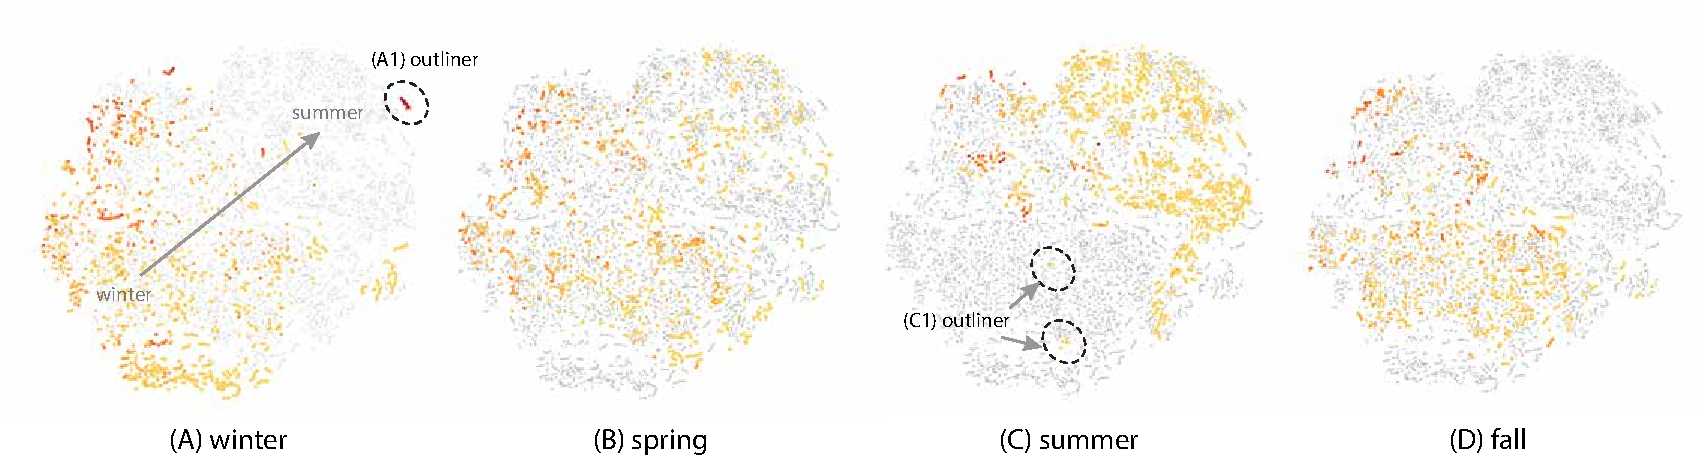
\includegraphics[width=0.45\textwidth]{figure/MultiRNNExplorer/Evaluation/seasonal_behavior.pdf}
	\vspace{-3mm}
	\caption{Projection View across four seasons whose time range are defined by local standards.}
	\label{fig:seasonal_feature}
	\vspace{-4mm}
\end{figure}

\subsubsection{Feature importance}
We select the individual sequences of Fig.~\ref{fig:teaser}D$_2$ and re-sort the features by the importance. 
From the Feature Importance View, the top important features are listed as Fig.~\ref{fig:teaser}C, and we observe that most of them are related to feature $\color{SO2Color}{SO_{2}}$ and \textit{\color{WINDColor}{Wind Speed}}.
Then, top features change to $\color{SO2Color}{SO_2}$ and $\color{PM25Color}{PM_{2.5}}$ in later epochs. 
This observation shows that feature importance may vary across different individual cases. 
By default without selecting any sequences, the features are ranked according to their average importance over of all the test cases. 
We find that the \textit{\color{WINDColor}{Wind Speed}} is a major factor that influences the forecast because the wind related features are ranked in front.
% ~\yh{how? larger wind speed indicates higher predicted value?}. 
The domain experts point out that as there are very few factories in Hong Kong, the local emissions are not a major reason that influences the forecast result. 
Instead, the $PM$ pollutants are easily transported from the north, west, and east of mainland China, thus the $wind$ plays an important role in the forecast of $\color{PM25Color}{PM_{2.5}}$ and $\color{PM10Color}{PM_{10}}$.
% 0.76
% \begin{figure*}[ht]
% 	\centering
% 	\includegraphics[width=1\textwidth]{pictures/Evaluation/winter_exploration.pdf}
% 	\vspace{-3mm}
% 	\caption{
% 	Case exploration for the $PM_{2.5}$ forecast in winter. A, B) Filter and highlight the individual cases in January 2018; C1, C2) Two groups of individual cases are selected by brushing; D) The top 10 importance features for the group selected in C1; E1, E2) Representative cases of C1 and C2.}
% 	\label{fig:winter_exploration}
% 	\vspace{-4mm}
% \end{figure*}

\begin{figure}[t]
	\centering
	\includegraphics[width=0.45\textwidth]{figure/MultiRNNExplorer/Evaluation/winter_exploration.pdf}
	\vspace{-3mm}
	\caption{Case exploration for the $PM_{2.5}$ forecast in winter. A, B) Filter and highlight the individual cases in January 2018; C1, C2) Two groups of individual cases are selected by brushing; D) The top 10 importance features for the group selected in C1; E1, E2) Representative cases of C1 and C2.}
	\label{fig:winter_exploration}
	\vspace{-4mm}
\end{figure}
During the exploration of different models, we notice that the temporal pattern of the Feature Importance View is very different across different models. 
Fig.~\ref{fig:gru_vs_rnn} compares the feature importance for vanilla RNN and GRU.
With the selected feature of \textit{100\_NE\_PM25}, one observation is that the Feature Importance Views of model GRU has a ``tail" (Fig.~\ref{fig:gru_vs_rnn}) especially for the first three timestamps, which is not observed in vanilla RNN.
% While the corresponding feature for vallina RNN have no such kind of pattern. 
This solves one question raised by the domain experts: is it necessary to use such complex models like RNN to conduct air pollutant forecasting tasks?
It is a controversial question~\cite{brownlee2017long} as in some applications all important information is included within within recent small time ranges~\cite{gers2002applying} and do not necessarily require complex machine learning models. 
By using our system, we can find that the GRUs are able to memorize more long-term information than vanilla RNNs. 
Since the air pollutant and meteorology features (such as temperature) have a daily periodic pattern, the input features around 24 hours ahead are also considered relevant to the forecast. 
In addition, since the GRU model have better performance compared with vanilla RNNs from Table~\ref{table:model_configuration}. 
% ~\yh{requires some logic to connect to gated RNN.}
We think the gate RNNs are applicable for the air pollutant forecast. 



\subsection{Case exploration}

In Hong Kong, air quality always have seasonal patterns such as the ``large winter-summer contrasts in $PM_{2.5}$ mass" due to the Asiatic monsoon~\cite{louie2005seasonal}. 
We conduct this case study to understand the model behavior in different seasons.  

\subsubsection{Overview of the model behavior across seasons}

% The Projection View allows users to select individual cases according to different times by brushing on the timeline (Fig.~\ref{fig:teaser}E) and provides an overview of all cases (\textbf{T5}).
In this case, we choose the GRU-Dense model and $PM_{2.5}$ as the target feature.
We switch the time ranges to filter the cases in winter, spring, summer, and fall. 
To highlight the selected cases, the unfiltered cases are then colored in light grey as shown in Fig.~\ref{fig:seasonal_feature}. 
We found that the fall and winter cases are clustered at the left-bottom part (Fig.~\ref{fig:seasonal_feature}A,D). 
The cases in summer are located at the right-top part (Fig.~\ref{fig:seasonal_feature}C), while the cases in spring are distributed in different locations compared with the other three seasons (Fig.~\ref{fig:seasonal_feature}B).
Despite some outliers exist in the Projection View as shown in Fig.~\ref{fig:seasonal_feature}A$_1$,C$_1$, the model is able to capture the complex seasonal features in data based on above observation. 

\subsubsection{Explore the model behavior in winter}

Furthermore, we notice that several cases indicate that the target location has a serious $PM_{2.5}$ pollutant in winter. 
In the Projection View, we first select the time ranges of January 2018 (Fig.~\ref{fig:winter_exploration}A) to highlight all the cases within this time range (Fig.~\ref{fig:winter_exploration}B). 
We notice there are many cases are colored in dark red, which indicates that these cases suffer a heavy $PM_{2.5}$ pollutant (Fig.~\ref{fig:winter_exploration}C1).
We select these cases to explore their feature importance distributions and rankings.
The top ten important features are \textit{\color{WINDColor}{Wind Speed}}, $\color{PM25Color}{PM_{2.5}}$ and $\color{PM10Color}{PM_{10}}$.
The selected cases also appear in the Individual Views; all these cases form one stack, and we choose one of them as an example as shown in Fig.~\ref{fig:winter_exploration}E$_1$. 
In the Cluster Importance Chart, cluster 3, 6, and 7 show great influence in the forecast. 
These corresponding feature clusters are shown in Fig.~\ref{fig:winter_exploration}E$_3$, which presents the clusters of $PM_x$ and \textit{Wind Speed} respectively. 
The above exploration further indicates that the most important features in the forecasting are about $\color{PM25Color}{PM_{2.5}}$, $\color{PM10Color}{PM_{10}}$, and \textit{\color{WINDColor}{Wind Speed}}. 

The domain experts state: ``During winter, strong radiative cooling over the continent creates a high-pressure anticyclone that drives cold, dry polar air from the continent into the surrounding oceanic areas, resulting in weak to moderate northeasterly winds or strong northerly winds" \cite{louie2005seasonal, murakami1979winter}. 
The weak to moderate wind is able to bring the air pollutant from Pearl River Delta region in China, which is a highly populated region and has a lot of heavy industry \cite{cao2003characteristics}.
Thus, the major factors that mostly influence Hong Kong's air quality in winter are the air pollutants and the wind.
Specifically, the $PM_{2.5}$ and $PM_{10}$ from the north and east affects the prediction results the most. 

We are also interested in comparing how the model generates prediction for the high-pollutant and low-pollutant cases in the winter. 
We select individual cases with low $PM_{2.5}$ from the Projection View as Fig.~\ref{fig:winter_exploration}C$_2$ shows, and the these cases appear in the Individual View. 
By observing the representative case (Fig.~\ref{fig:winter_exploration}E$_2$), we find the cluster 6 is very important at the last timestamp in the Cluster Importance Chart (Fig.~\ref{fig:winter_exploration}E$_4$), which indicates nearby $PM_{2.5}$ and $PM_{10}$. 
Both the Top Feature List (Fig.~\ref{fig:winter_exploration}E$_5$) and the Cluster Importance Chart show that the features of recent time steps are very important for the forecast, which is different from the heavy pollution cases (Fig.~\ref{fig:winter_exploration}E$_6$). 
We infer that for the low air pollutant cases, only recent important features are leveraged by the model. 











\section{Discussion and Conclusion}

In this paper, we presented MultiRNNExplorer, a visual analytic system for understanding RNN models for high-dimensional time-series forecasting.
Specifically, we use air pollutant forecasting as the target application. 
To understand the the model mechanism from a global perspective, we propose a technique to estimate the hidden units' response to an individual feature by measuring how different feature selections affect the hidden units' output distribution. 
From a finer granularity, we further use the gradient-based method to measure the local feature importance for each sequence instance. 
Based on these techniques, we design a visual analytic system which enables the users to explore and reason about the model behavior from different perspectives. 
Our evaluation includes three case studies that demonstrate the effectiveness of the proposed system for comprehensive analysis of RNNs.
Meanwhile, there are some issues need to be discussed:

\textbf{Scalability.}
Several views may suffer scalability issues when the number of cases increase. 
In Projection View, thousands of individual cases need to be visualized and cause serious visual clutter due to the overlap of circles.  
% Even though we provide interactions such as zoom and pan which enable the users to iteratively explore the cases, it is still difficult for the users to clearly observe the overview of the case similarity.  
In our case, more than 8000 points are visualized. 
If data size keeps increasing, we may also apply other advanced projection techniques\cite{van2017visual, pezzotti2016hierarchical} for Projection View. 
The individual view also has such a problem: it is easy for users to brush hundreds of individual cases from Projection View and generate tens of clusters. Due to the limited screen size, our current design allows 9 groups of individual cases to be shown at the same time and uses the scroll bar to enable the observation of more groups.
% Throughout the system, the feature type is encoded by categorical colors. Because humans suffer perception issues for more than 10 categorical colors, we manually choose similar colors for highly correlated features (for example, $PM_{2.5}$ and $PM_{10}$ are encoded by light green and dark green). For more features, we may need only a few colors for the features of interest and encode other features by the same color (for example, gray). 

\textbf{Generalization.}
Though we use air pollutant forecasting as example in this paper, the proposed method can be easily extended to other high-dimensional time-series forecasts with few changes. 
The only design that may need to be fine-tuned to is feature glyphs (Fig.~\ref{fig:cluster_design}).
The current design supports encoding three spatial attributes including direction, type, and distance and more design choices can be explored according to different requirements in other domains. 
% Any other cell-like glyph design is also applicable in our method. 


% There is some promising future work for MultiRNNExplorer. 
There are also some future directions to improve MultiRNNExplorer.
% First, improve the efficiency of the response estimation. With 8375 test cases, the current method needs hours of calculation which has to be done offline. 
% In the future work, we will improve this method by introducing rational sampling techniques or develop alternative estimation techniques to enable our system to support realtime data processing. 
One approach is to improve the individual comparison. 
In our current design, the individual comparison requires comparing data instances side by side. 
Supporting interactions to highlight the differences would further benefit users in this scenario.
% A specific comparison design will be helpful to ease the burden of users. 
We also consider to use our system on other high-dimensional forecasting applications including such as fraud detection\cite{jurgovsky2018sequence}. 
We are also exploring the possibility of applying MultiRNNExplorer to audio modeling tasks. 



% \chapter{Conclusion and Future Work}

The fast increasing global urbanization process in recent years has greatly changed the world in the recent 50 years. The human migration from the rural area to the urban area results in a series of problems such as environment pollutant, traffic jam and insufficient local resource supply. Meanwhile, with the development of science and technology, a variety of data source can be collected easier and cheaper, which also provide the opportunity for analysts to understand the phenomenon and solve the problems. Although a lot of automatic techniques have been proposed in recent years, most of them still have limitations such as the lack of interpretability, difficulty in handling unexpected cases. Due to the variety of urban applications, these techniques always generate uncontrollable results which is hard to be accepted by the non-expert users. Thus the human experience and knowledge are required to make judgement or provide guidance in the analyzing process. Visual analytics, integrating the intuitive graphics and auto techniques, bridge the gap between users and complex urban data by taking human into the analysis loop.  

This thesis consists of three works that cover the three domains of urban information: place, people and technology. We start with a brief summary of the existing visualization techniques used in urban data exploration. After that, we introduced three visual analytics system target at the human-scale urban form exploration, large scale movement visualization and urban computing technique interpretation.

In Chapter 2, we introduce Streetvizor, a framework enabling urban analysts to explore the human scale urban from city-, region- and street-level. The proposed system takes the street view images as input and extracts human-scale urban form features by leveraging the advanced machine learning techniques. Then, a visual analytics system is built upon the urban form feature database. The proposed method is evaluated by the real world data from four cities: London, Singapore, Hong Kong, and New York City. 

In Chapter 3, we have developed RAEB(route aware edge bundling), a novel edge bundling technique to visualize the overview of a large amount of OD trails in urban traffic data. Target at the limitation of traditional edge bundling techniques, we introduce the urban traffic network as a constraint to the trail bundles. A series of new parameters are employed in the pipeline.

In Chapter 4, we propose MultiRNNExplorer, a visual analytics system which helps analysts to understand the RNNs in high-dimensional time series forecast. The visual analytics system aims to interpret RNNs from two aspects, the overall model mechanism and the feature importance. Several case studies on air pollutant forecast show the effectiveness of the proposed technique.

Even though several novel designs and comprehensive analytics systems have been discussed in this thesis, the current development of urban related visualization techniques still cannot meet the analysis requirement due to the increasing complexity and variety of the applications. Based on the current work, we list several promising future directions.

\textbf{High-level urban analysis based on street view images.} In Chapter 2, we discuss how to leverage the easily collected street view images and advanced machine learning techniques to help us build the comprehensive visual analytics system for human-scale urban form explorations. In the future, we will extend the current framework to the more complex tasks. For example, an exiting research work uses vehicle classification techniques to estimate the demographic makeup of the US; We can also extract the signboards and building style from the street view images to support the exploration of urban region  functionalities.  

\textbf{Improve the bundling and rendering efficiency for the large trajectory dataset.} In Chapter 3, the edge bundling and rendering process still require tens of seconds to finish the visualization tasks, which makes the interactive exploration impossible. Our proposed technique is built upon the kernel density estimation techniques which can be parallelized. In the future, we will use the GPU-acceleration to improve bundling efficiency. In addition, to improve the computing efficiency, another strategy is to reduce the data amount. Traditional sampling methods, such as uniform and stratified sampling, cannot keep visualization accuracy. We plan to develop visualization aware sampling techniques to support the fast OD trails bundling. 

\textbf{Support model ensemble exploration.} Due to the complexity and variety of urban information exploration, a single forecast technique is always not enough to produce a credible and accurate result. In the future, we will extend the technique interpretation from RNNs to technique ensembles. However, use the same criteria to interpret multiple techniques is difficult due to the different algorithm mechanisms. Thus, we plan to figure out some uniform properties of these techniques (such as the feature importance) to make the them comparable. 


% \chapter{Introduction}\label{sec-introduction}

MapReduce is a successful paradigm~\cite{Dean2008}, originally proposed by Google,
for the ease of distributed data processing on a large number of machines.
In such a system, users specify two functions:
(1) a {\em map} function to process an input key/value pair,
and to generate a set of intermediate key/value pairs;
(2) a {\em reduce} function to merge all intermediate key/value pairs associated with the same key.
The system will automatically distribute and execute tasks on multiple machines~\cite{HADOOP, Dean2008}
or multiple CPUs in a single machine~\cite{Ranger2007}.
Thus, this paradigm reduces the programming complexity so that developers can easily
exploit the parallelism in the underlying computing resources for complex tasks.
Encouraged by the success of CPU-based MapReduce systems, in particular, Phoenix~\cite{Ranger2007},
we develop Mars, a MapReduce system accelerated with graphics processors, or GPUs.

GPUs can be regarded as massively parallel processors with an order of magnitude higher computation
power (in terms of number of floating point operations per second) and memory bandwidth than CPUs~\cite{Ailamaki2006}.
%Moreover, the performance of GPUs is improving at a rate higher than Moore's law for CPUs.
\red{Moreover, the computational performance of GPUs is improving at a rate higher than that of CPUs.}
However, it is a challenging task to program GPUs for general-purpose computing applications, including
those that MapReduce users are familiar with. Specifically, GPUs are traditionally designed as
special-purpose co-processors for dedicated graphics rendering. As such, GPU cores are SIMD
(Single-Instruction-Multiple-Data), which discourages complex control flows. Furthermore, GPU cores are virtualized, and threads are managed by the hardware. Finally,
GPUs manage their own on-board device memory and require programmers to explicitly
transfer data between the GPU memory and the main memory.  Additionally, the architectural details
of GPUs vary by vendors as well as by product releases, and programmer's access to these details is limited.
All these factors make desirable a GPGPU (General Purpose Computation on GPUs) framework
on which users can develop correct and efficient GPU programs easily.

Recently, several GPGPU programming frameworks have been introduced, such as NVIDIA CUDA~\cite{CUDA}, and AMD Brook+~\cite{BROOKPLUS}.
\red{These frameworks significantly improve the programmability of GPUs; nevertheless, their interfaces are vendor-specific and their hardware abstractions may be unsuitable for complex applications such as those running on MapReduce.
Therefore, we propose Mars, a MapReduce framework to ease the programming of such applications on the GPU.} Furthermore, the MapReduce framework of Mars enables the integration of GPU-accelerated code to distributed environment, like Hadoop, with the least effort.
Our Mars system can run on multi-core CPUs (MarsCPU), on CUDA-enabled NVIDIA GPUs (MarsCUDA) or Brook+-enabled AMD GPUs (MarsBrook), or on a combination of a multi-core CPU and a GPU on a single machine.
We further integrate Mars into Hadoop~\cite{HADOOP}, an open-source CPU-based MapReduce system on a
network of machines, which results in MarsHadoop, where each machine can utilize its GPU with MarsCUDA or MarsBrook
in addition to its CPU with the original Hadoop. No matter what GPU and/or CPU Mars runs on, the API (Application
Programming Interface) to the user is the same and is similar to that of existing CPU-based MapReduce systems.

Easing up GPU programming for MapReduce applications is the main goal of our work. However, a higher-level
abstraction for programming, specifically MapReduce, comes at a price of performance.
In particular, we identify the following three technical challenges in implementing Mars on GPUs.
%First, since MapReduce divides up a task by data, data skews are an inherent problem in utilizing
First, since MapReduce divides up a task by data, load imbalance is an inherent problem in utilizing
the massive thread parallelism on the GPU, especially because GPU threads are managed by the hardware.
\red{Second, GPUs lack efficient global synchronization mechanisms. Threads in Map or Reduce tasks are likely to have write conflicts on the output buffer.
%Although NVIDIA GPUs provide atomic operations on the global memory, the performance of these atomic operations is so poor that using them performs worse than using the CPU \cite{ATOMIC}. Therefore, the overhead of atomic operations harm the scalability of massive GPU threads.
While atomic operations are enabled in recent GPUs, the overhead of atomic operations would harm the scalability of massive GPU threads \cite{ATOMIC}. We consider a lock free scheme to minimize the synchronization overhead among GPU threads.}
%It is desirable to implement a extremely low-overhead thread synchronization mechanism.
%Therefore, it is mandatory to implement thread synchronization, and the synchronization overhead must be low so as to scale to the massive number of GPU threads.
Third, MapReduce applications are in general data-intensive and their result sizes are data-dependent. These two characteristics pose the following requirements on programming the GPU: (a) sufficient  thread parallelism to hide the high latency and to utilize the high bandwidth of the device memory; (b) pre-allocation of output buffers in the device memory for bulk DMA transfers, as GPU memory allocation is done through the CPU before the GPU program starts.

With these challenges in mind, we develop Mars for GPUs of two most
common programming interfaces - CUDA and Brook+. We focus on
MarsCUDA, than MarsBrook, because in our implementation
and evaluation, CUDA was more flexible and had a higher performance than Brook+
for MapReduce applications.

In MarsCUDA, the massive thread parallelism on the GPU is well utilized
as each thread is automatically assigned a key/value pair to work on.
In {\em Map}, the system evenly distributes key/value
pairs to each thread. In {\em Reduce}, we develop a simple but effective
\red{skew handling scheme to re-distribute data evenly across all reduce tasks. }To avoid write conflicts between
threads, we adopt a lock-free scheme that guarantees the
correctness of parallel execution with little synchronization
overhead. 

We extend our general design of Mars from a GPU-only MapReduce framework to a MapReduce system with GPU acceleration enabled. With this extension, Mars components can work stand-alone on a single platform, e.g., MarsCUDA on a CUDA-enabled GPU or MarsCPU on a multi-core CPU, as well as to work together to utilize multiple processors, e.g., a CPU and a GPU on a single machine.
We also integrate Mars into Hadoop to enable GPU-acceleration for individual machines in a distributed environment.

\red{We evaluated the performance of Mars in comparison with its CPU-based counterparts and the native implementation without MapReduce. Our results demonstrate the effectiveness of our  GPU-oriented  optimization  strategies. On average, our MarsCUDA is 22 times faster than the CPU-based MapReduce, Phoenix~\cite{Ranger2007}, and is less than 3 times slower than the hand-tuned native CUDA implementation. Additionally, the applications developed with Mars had a code size reduction up to seven times, compared with hand-tuned native CUDA code.}

\textbf{Organization:} The remainder of the thesis is organized as
follows. We give a brief overview of GPUs, and review prior work on GPGPU and
MapReduce in Chapter~\ref{sec-preliminaries}. We present the design
and implementation details of Mars in Chapter~\ref{sec-design} and
Chapter~\ref{sec-implement} respectively. We present the extension
to multiple machines in
Chapter~\ref{sec-beyond}. In Chapter~\ref{sec-eval}, we present our
experimental results. Finally, we conclude in Chapter~\ref{sec-conclusion}.

\newpage

% \chapter{Preliminaries and Related Work}\label{sec-preliminaries}

In this chapter, we first give a brief introduction on the GPU, and then review the related work on GPGPU as well as on MapReduce.


\section{Graphics Processing Units (GPUs)}

The GPU is an integral component of
modern computers, ranging from handheld devices to high-end servers.
GPUs are originally designed for gaming applications with fixed
hardware pipelines for rendering. Due to the high computation power
and rapidly improving programmability, they have recently become a
powerful co-processor for general purpose computing~\cite{Ailamaki2006}.
%For example, NVIDIA Tesla GPU series have been
%adopted to high performance computers and clusters~\cite{Tesla}. For
%more details on the GPU and its programming techniques, we refer the
%reader to a recent book edited by Nguyen~\cite{GPUGems}.


\begin{figure}[ht]
\centering
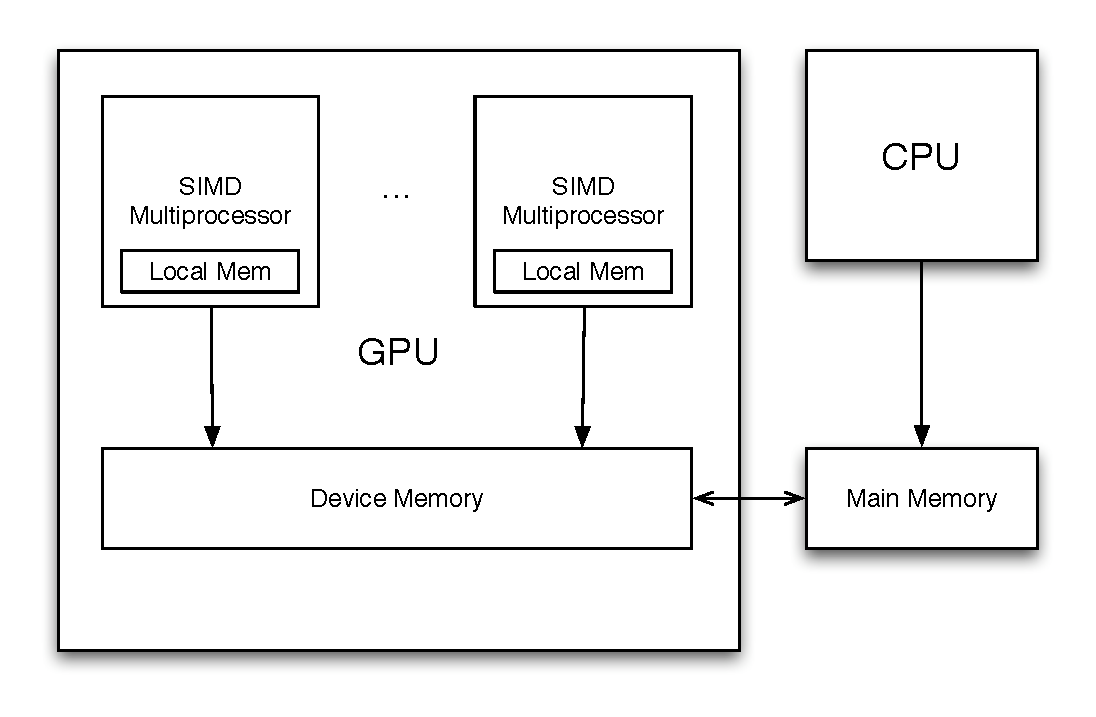
\includegraphics[width=0.65\textwidth]{figure/gpuarch.eps}
\caption{The many-core architecture model for GPUs}
\label{fig:manycore}
\end{figure}



%The major vendors such as NVIDIA and AMD provide similar programmable hardware pipelines, and develop similar programming frameworks.
As shown in Figure \ref{fig:manycore}, we model the GPU as a many-core processor, which
contains a number of SIMD multiprocessors.
Such a many-core model is common to both AMD and NVIDIA GPUs.
On the GPU board, there is a GRAM device memory.
The device memory has both a high bandwidth and a high access latency.
For example, the NVIDIA GTX280 GPU has an access latency of 400 to 600 cycles, and
the peak memory bandwidth between the device memory and the multiprocessors
is around 140 GB/second.

Both NVIDIA CUDA and AMD Brook+ expose a parallel programming model, which does not require programmers to have knowledge of the
graphics rendering pipeline. In this model, the system consists of a
{\em host} (a CPU), and one or more {\em devices} (GPUs).
GPUs are abstracted as massively data-parallel co-processors.
CUDA and Brook+ programmers write code using C/C++ syntax with extended keywords for kernel functions,
which are GPU programs to be executed on {\em devices}.

Programming frameworks such as CUDA and Brook+ greatly improve
the programmability of the GPU.
However, it is still a challenging task of developing efficient GPU programs for complex applications, such as those with MapReduce, because GPUs have a special-purpose co-processor architecture and are vendor-specific on the programming frameworks for complex applications.
\red{Although the newly introduced OpenCL~\cite{OPENCL} is an industry standard further hiding hardware details from users, Mars is at a higher level of abstraction.} OpenCL is a general-purpose programming language, with which Mars or other MapReduce frameworks can be developed.

\section{GPGPU}




GPGPU, or General Purpose Computation on GPUs, has recently emerged
in various applications, such as linear algebra~\cite{Jiang2005,Volkov2008}, embedded system design~\cite{Feng2007}, bioinformatics~\cite{Charalambous2005}, databases~\cite{Govindaraju2006,Govindaraju2004,He2008a}, machine learning~\cite{Chu2006}, and
distributed computing projects including Folding@home and Seti@home.
Recently, several GPGPU languages including AMD Brook+~\cite{BROOKPLUS} (extended from Brook~\cite{Buck2004}) and NVIDIA
CUDA~\cite{CUDA} have been proposed by GPU vendors. They usually
expose a general-purpose, massively multi-threaded computing
architecture and provide a programming environment similar to C/C++.
High-level programming frameworks such as Accelerator~\cite{Tarditi2006} and RapidMind~\cite{McCool2006} are also
developed to better facilitate GPGPU programming. These
programming frameworks require programmers to have knowledge of specific
programming models such as the stream programming model in Brook+~\cite{Buck2004}, or even more, knowledge of the GPU hardware
details. By contrast, we propose to develop a MapReduce framework accelerated with
GPUs to ease the development of a more complex class of data
processing tasks. It provides a uniform MapReduce interface no matter whether it runs on the GPU, on the CPU, or both.

We now briefly survey recent  work that developed GPGPU primitives as building blocks for various applications, in particular, those not covered in the survey by Owens et al~\cite{Owens2007}.
Sengupta et al.~\cite{Sengupta2007} proposed the segmented scan primitive.
He et al.~\cite{He2007} proposed a multi-pass scheme to optimize the scatter and the gather operations.
He et al.~\cite{He2008a} further developed a small set of primitives such as prefix sum and split for relational databases.
Additionally, CUDPP~\cite{CUDPP}, a CUDA library of data parallel primitives, was released for GPGPU computing.
These GPU-based primitives reduce the complexity of GPU programming.
However, even with the primitives, programmers need to write complex GPU code for data processing tasks.
By contrast, our work further simplifies GPU programming for MapReduce programmers by providing them with a higher level and more familiar interface than the primitives.

\red{This thesis focuses  on  accelerating  MapReduce  on  the  GPU,  and  provides  a  GPU-based MapReduce framework to developers. As in the original MapReduce,  it  is  up  to  developers'  choice  whether to  use  MapReduce  or  not  according  to the workload's computational characteristics. Recent studies \cite{Kerr2010}  have used data analysis techniques to categorize the computational characteristics of different workloads on the GPU. These techniques are helpful for developers to determine whether their workloads are suitable for Mars in
specific and the GPU in general.}

%Our previous study on Mars~\cite{He2008} implemented the MapReuduce framework on CUDA-enabled GPUs. This work extends the previous work in two major aspects. First, we extend the CUDA-only Mars to another large group of GPUs, so that it can run on both NVIDIA and AMD GPUs. Second, we use GPU-only Mars as a component to work with CPU-based Mars on a single machine, as well as with Hadoop in a distributed environment.

\section{MapReduce}
The MapReduce framework~\cite{Dean2008} is based on two primitives, Map and Reduce, from functional programming.
The general form is as follows:
\begin{quote}
\tab \bf{Map:} $(k_1, v_1) \rightarrow list(k_2, v_2)$.

\tab \bf{Reduce:} $(k_2, list(v_2)) \rightarrow list(k_3, v_3)$.
\end{quote}



The Map function takes an input key/value pair $(k_1, v_1)$ and outputs a list of intermediate key/value pairs $(k_2, v_2)$.
The Reduce function takes all values associated with the same key and produces a list of key/value pairs.
Programmers implement the application logic inside the Map function and the Reduce function.
The MapReduce runtime manages the parallel execution of these two functions.



The following pseudo code illustrates a program written using MapReduce.
This program counts the number of occurrences of each word in a collection of documents~\cite{Dean2008}.
In this program, {\em Map} and {\em Reduce} are implemented using two system-provided APIs, {\em EmitIntermediate} and {\em Emit}, respectively.

\begin{quote}
{\bf Map}(void *{\em doc}) \{ \\
1: {\bf for} each word {\em w} in {\em doc} \\
2: \hspace{3mm} {\bf EmitIntermediate}({\em w}, {\em 1}); // count each word once \\
\} \\
{\bf Reduce}(void *{\em word}, Iterator {\em values}) \{ \\
1: int {\em result} = 0; \\
2: {\bf for} each {\em v} in {\em values} \\
3: \hspace{3mm} {\em result} += {\em v}; \\
4: {\bf Emit}({\em word}, {\em result}); // output {\em word} and its count \\
\}
\end{quote}

%\begin{quote}
%\tab {\bf Map}(void *{\em doc}) \{ \\
%\tab 1: \tab {\bf for} each word {\em w} in {\em doc} \\
%\tab 2: \tab \tab {\bf EmitIntermediate}({\em w}, {\em 1}); // count each word once \\
%\tab \} \\
%\tab {\bf Reduce}(void *{\em word}, Iterator {\em values}) \{ \\
%\tab 1: \tab int {\em result} = 0; \\
%\tab 2: \tab {\bf for} each {\em v} in {\em values} \\
%\tab 3: \tab \tab {\em result} += {\em v}; \\
%\tab 4: \tab {\bf Emit}({\em word}, {\em result}); // output {\em word} and its count \\
%\tab \}
%\end{quote}

There have been several MapReduce implementations since MapReduce was proposed~\cite{Dean2008}.
Hadoop~\cite{HADOOP} is an open-source MapReduce implementation on clusters.
Based on Hadoop, Yang et al.~\cite{Yang2007} added the merge operation to MapReduce for the ease of relational databases operations.
Phoenix~\cite{Ranger2007} is an efficient MapReduce runtime system on multi-core CPUs.
Kruijf et al.~\cite{Kruijf2007} developed MapReduce on the Cell BE.
Yeung et al.~\cite{Yeung2008} implemented an FPGA-based MapReduce system.

\red{Let us briefly introduce the implementation of Phoenix~\cite{Ranger2007}. A key component in Phoenix is a scheduler, for buffer management and task distribution. The scheduler starts the Map stage by evenly dividing the input buffer into small chunks, and assigns the chunks to map workers dynamically. Each map worker runs in a CPU thread. The Reduce stage does not start until all Map tasks are done. The scheduler groups the intermediate output from the Map stage by key, and a Reduce worker processes values associated with the same key. Reduce tasks are assigned to workers dynamically. Each reduce worker maintains a static array for outputting results, and sorts this static array using insertion sort. Finally, the scheduler merges all output arrays of reduce workers into a single one. Because the output data size is not known in advance, the scheduler first allocates buffers with a default small size, and then resizes the buffer as needed.}


%Our previous work on Mars implemented MapReduce on CUDA-enabled GPUs~\cite{He2008}. 
Catanzaro et al.~\cite{Catanzaro2008}, developed another MapReduce system on the GPU, but it required programmers to be aware of GPU hardware details, such as thread configuration and memory hierarchy.
Finally, the Merge framework~\cite{Linderman2008}, focused on dynamically scheduling MapReduce tasks among multiple processors, dedicated to Intel products.
By contrast, Mars hides hardware details from programmers, and works on heterogeneous GPUs, a combination of CPU and GPU on a single machine, as well as a distributed system of multiple machines.

\newpage

% \chapter{Design of Mars} \label{sec-design}

In this chapter, we present our design for Mars, with emphasis on the GPU-based component.
Our design is guided by the following three goals.

\begin{enumerate}
  \item {\em Programmability}. User code size reduction encourages programmers to use the GPU for their tasks.
  \item {\em Flexibility}. The design should be applicable to various multi-/many-core processors, e.g., multi-core CPUs and AMD GPUs, and should be as expressive as the underlying runtime, e.g., NVIDIA CUDA, AMD Brook+ or pthreads, so that the system will work for a wide range of hardware and applications.
  \item {\em High Performance}. The overall performance should be accelerated by the GPU effectively.
\end{enumerate}

\section{Overview}
\red{By examining the Phoenix design, we see that there are three potential sources of overhead.  First, the tight-coupling of the Map and Reduce stages makes every application go through both stages, no matter whether they need both stages or not. Second, a dynamic thread scheduler for task assignment heavily relies on locking to implement synchronization. Third, each reduce worker may require frequent data movement for sorting the static output array, and the data movement can become a bottleneck for the overall performance. The latest paper about Phoenix also points out this problem~\cite{Yoo2009}.}


In the Mars design, we decide to separate a MapReduce workflow into three loosely coupled stages -
{\em Map}, {\em Group} and {\em Reduce}. The {\em Group} stage is designed to group {\em Map} output by key, which is the format for {\em Reduce} input. Our observation is that some applications need only the
{\em Map} stage, some need both {\em Map} and {\em Group}, and some need all of the three stages.
\red{The Group stage is the same as running Reduce with the identity function in the original MapReduce system \cite{Dean2008}.
Our purpose of providing an explicit Group stage is to allow a MapReduce application with high flexibility to customize its workflow,
and to avoid the overhead of entering unnecessary stages. }
No matter what configuration of the three stages is for an application, the MapReduce interface
of Mars is unchanged - users write Map and/or Reduce functions when necessary.

Moreover, we decide to use a lock-free scheme for synchronization
and to perform in-advance buffer allocation. One reason is to
avoid heavy overheads of locking and buffer reallocation. The
other reason is that, current GPUs do not support locking
or in-flight buffer reallocation. In our design, we statically
distributes tasks to a massive number of GPU threads, so that we
can fully utilize the parallelism of the GPU. We adopt a two-phase,
lock-free scheme for result output. The basic idea is that, in the
first phase, we calculate histograms on the size of output results for each
thread, followed by a prefix sum operation on the histograms,
so that we obtain both the exact output buffer size and the deterministic
write position for each thread; in the second phase, we
perform the actual computation and output. We will detail this strategy in
Section~\ref{sec-lockfree}.

\section{Data Structure} \label{sec-datastructure}
Data structures in Mars affect the workflow, memory access patterns, and the expressiveness of the system.

Since the GPU does not support dynamic memory allocation on the
device memory during the execution of the GPU code, this limitation rules out
 dynamic data structures such as queues and linked lists, as used in
other MapReduce implementations. Instead, we use plain arrays as the
main data structure in Mars. The {\em Map} stage takes input records in
the key/value form, and outputs intermediate result records, which
are in turn the input of the {\em Group} stage. The output of the {\em Group}
stage is the input of the {\em Reduce} stage, and {\em Reduce} produces final output
records. Each of the three sets - the input records, the intermediate records and the
output records  - is stored in three arrays, i.e., the
key array, the value array and the directory index array. The
directory index consists of an entry of $<$key offset, key size,
value offset, value size$>$ for each key/value pair. Given a
directory index entry, we fetch the key or the value at the
corresponding offset in the key array or the value array.

Variable-sized types, such as strings, are supported with the directory index, since current GPUs have no such build-in types yet. If
two key/value pairs need to be swapped, we swap their corresponding
entries in the directory index without modifying the key and the
value arrays.

Some applications perform chained MapReduce procedures,
where the output of one MapReduce procedure is the input of
another one. Since the sets of
input records, intermediate records and output records  are all
in the three-array structure uniformly, chained MapReduce is
supported gracefully in Mars.

\section{Mars Workflow}
Figure \ref{fig:MarsWorkflow} illustrates the workflow of Mars, assuming the data resides in the disk at the beginning.
The Mars scheduler runs on the CPU, and schedules tasks to the GPU.
Mars has three stages, {\em Map}, {\em Group}, and {\em Reduce}.

\begin{figure}[ht]
  \centering
  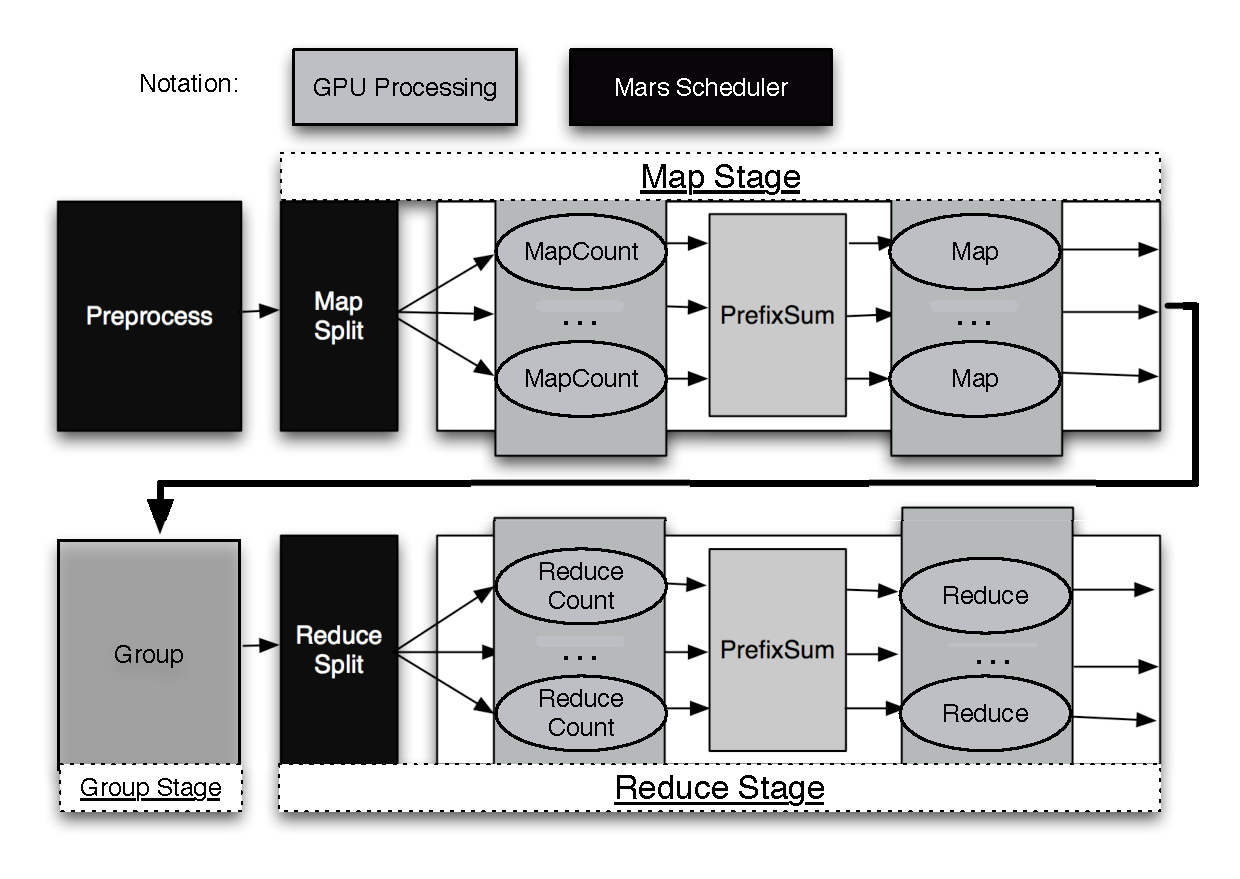
\includegraphics[width=0.60\textwidth]{figure/Mars_workflow.eps}
  \caption{The workflow of Mars on the GPU. }\label{fig:MarsWorkflow}
\end{figure}

Before the {\em Map} stage, Mars preprocesses on the CPU the input data from disk,
transforming the input data to key/value pairs (input records) in main memory.
After that, it transfers input records from the main memory to the GPU device memory.

In the {\em Map} stage, {\em Map Split} dispatches
input records to GPU threads such that the workload for all threads is even.
Each thread executes the user-defined MapCount function to compute a local histogram on
the number and the total size of intermediate records that {\em Map} will output.
Then, the runtime performs a GPU-based {\em Prefix Sum} on the local histograms to
obtain the output size and the write position for each thread.
Finally, after the CPU allocates the output buffer in the device memory, each GPU
thread executes the user-defined Map function and outputs results.  Since the write
position for each thread is pre-computed and has no conflict with any other threads,
there will be no write conflict between concurrent threads. This lock-free scheme of MapCount,
Prefix Sum, and Map is adapted from our previous
work~\cite{He2008a}.

\red{In the {\em Group} stage, both sort-based and hash-based approaches are available for grouping records by key. However, we adopt the sort-based, because some applications require to sort all output records, and the hash-based approach has to perform additional sort within each hash bucket. }


In the {\em Reduce} stage, {\em Reduce Split} dispatches each group of records
with the same key to a GPU thread.
However, it may cause load imbalance between threads, since the number of records of different groups may vary widely.
We adopt a skew handling scheme to alleviate the load imbalance problem (Section~\ref{sec-reduce}).
The {\em Reduce} stage then works in a lock-free scheme, similar to that in {\em Map}, to obtain the result size and the write location for each thread.
Finally, all Reduce workers output results to a single buffer.

Because these three stages are loosely coupled and not every application requires all
stages, Mars allows users to customize the following workflows in their applications:
\begin{itemize}
\item MAP\_ONLY. Mars executes the {\em Map} stage only, and does not execute the {\em Group} or {\em Reduce} stage.
\item MAP\_GROUP. Mars executes the {\em Map} and {\em Group} stages, and does not execute the {\em Reduce} stage.
\item MAP\_GROUP\_REDUCE.  Mars executes all three stages -- {\em Map}, {\em Group}, and {\em Reduce} stages.
\end{itemize}

Because usually applications need a Map to transform input records, and a Group to
prepare for the intermediate records to feed to Reduce, we exclude the other
workflow configurations that skip either Map or Group in the presence of Reduce.

\section{Lock-free Scheme} \label{sec-lockfree}

With the array structure, we allocate the space on the device memory
for the input data as well as for the result output before executing
the GPU program. However, the sizes of the output from the {\em Map} and
the {\em Reduce} stages are unknown. Moreover, write conflicts occur when
multiple threads write results to the shared output array. To
address these two problems, we adopt a previous lock-free output
scheme for relational joins~\cite{He2008a}. Since the output scheme
for the {\em Map} stage is similar to that for the {\em Reduce} stage, we
present the scheme for the {\em Map} stage only.

First, each MapCount invocation on a thread outputs three counts, i.e.,
the number of intermediate results, the total size of intermediate keys (in bytes)
and the total size of intermediate values (in bytes).
Based on intermediate key sizes (or value sizes),
Mars computes a prefix sum on these sizes and produces an array of write locations.
A write location is the start location in the output array for a map task to write.
Based on the number of intermediate results,
Mars computes a prefix sum and produces an array of start locations in the output
directory index.
Through these prefix sums, we also know the sizes of the arrays for the intermediate
results.
Finally, Mars allocates arrays in the device memory with the exact sizes for
storing the intermediate results.

Second, each Map invocation on a thread outputs the intermediate key/value pairs to
the output array.
Since each Map has its deterministic and non-overlapping positions to write to,
the write conflicts are avoided.


The lock-free scheme is suitable for the massive thread parallelism on the GPU, even
though it performs a MapCount in addition to a Map. The overhead of executing MapCount
is application dependent, and is usually small. For example, this overhead is negligible
in the matrix multiplication in our study, since MapCount simply emits the size without
performing the actual multiplication. In addition, the code for MapCount function is also application dependent, while in most cases, programmers write one statement to emits output data sizes. 

\red{
\section{Rapid Group} \label{sec-rapid}
The Group stage requires to sort intermediate records.
However, we observe that some applications inherently have their intermediate records grouped after the Map phase, and each group has the same number of records.
For example, [A,A,A,B,B,B,C,C,C] shows three groups with A, B, and C as the key respectively, and each group is with the same size 3.
For such applications, Mars provides a configuration parameter for users to indicate whether the intermediate data is already grouped. The runtime automatically skips the time consuming sorting, and then dispatches each group of intermediate records with the same group size to Reduce workers.
We name this strategy as ``Rapid Group".
}

\section{Skew handling} \label{sec-reduce}

We design a skew handling scheme to distribute workloads evenly across reduce workers, where the user-defined Reduce operation is commutative and associative.
This scheme iteratively performs the {\em Reduce} stage in the following two steps.  First, we divide the data into $M$ equal-sized chunks.  Second, we perform a reduction on each chunk. In this step, each of the $M$ threads applies the reduce function on groups of records in a single chunk.  Note, in each iteration, we perform reduction on the intermediate results with the same keys only.

%This scheme starts within the {\em Group} stage, immediately after the sorting, and performs in the following three steps.  First, we divide the data into $M$ equal-sized chunks. Second, we perform a reduction on each chunk.  In this step, each of the $M$ threads applies the reduce function on groups of records in a single chunk, called {\em local reduction}.  Finally, we group the reduced intermediate results and pass them to the {\em Reduce} stage.  This skew handling scheme makes sure that {\em local reduction} in {\em Group} stage are load-balanced.  Additionally, the {\em Reduce} stage processes compact groups of records, so that it alleviates the bottleneck caused by the largest group.

\section{Mars APIs}
Mars provides a small set of APIs. Similar to the existing MapReduce
frameworks, Mars has two kinds of APIs, the user-implemented APIs,
which the users should implement by themselves, and the
system-provided APIs, which the users can use as library calls.
%We refer the readers to our conference paper~\cite{He2008} for more details about Mars APIs.
The definitions of these APIs are in Table \ref{tb:marsapi}.

\doublerulesep 0.1pt
\begin{table}[htb]
  \centering
 \linespread{1.7}{ {\footnotesize
  \caption{Mars APIs}\label{tb:marsapi}
\vspace{2em}
  \begin{tabular}{p{5cm}p{7.5cm}p{3.5cm}}
  \hline
\noalign{\smallskip}
   \textbf{Function Name} & \textbf{Description} & \textbf{Function Type}\\
\noalign{\smallskip}
  \hline
   MAP\_COUNT & It calculates the output buffer size of MAP. & User-implemented \\
   MAP & The map function. & User-implemented \\
   REDUCE\_COUNT & It calculates the output buffer size of REDUCE. & User-implemented \\
   REDUCE & The reduce function. & User-implemented \\
   EMIT\_INTERMEDIATE\_COUNT & It emits the key size and the value size in MAP\_COUNT. & System-provided \\
   EMIT\_INTERMEDIATE & It emits the key and the value in MAP. & System-provided \\
   EMIT\_COUNT & It emits the key size and the value size in REDUCE\_COUNT. & System-provided \\
   EMIT & It emits the key and the value in REDUCE. & System-provided \\
\noalign{\smallskip}
  \hline
  \end{tabular}
  }}
\end{table}



\newpage

% \chapter{Single-Machine Implementations}\label{sec-implement}
In this chapter, we present the implementation details of Mars on a
single machine. The current Mars system consists of four modules
(Table \ref{tb:impls}). All these four modules share the common
design of Mars, and provide the same MapReduce interface to the
user. They can run on different hardware platforms: MarsCUDA on
an NVIDIA GPU, MarsBrook on an AMD GPU, MarsCPU on a multi-core CPU,
and the GPU/CPU co-processing module on both the CPU and the GPU
through combining the aforementioned modules.  Different modules in
Mars allow programmers to take advantage of different processors on
a single machine. Because our machines cannot host a multi-GPU configuration due to limited extension slots, we have not explored multi-GPU co-processing.

\begin{table}[htb]
  \centering
 \linespread{1.7}{ {\footnotesize
  \caption{Modules in the Mars system}\label{tb:impls}
\vspace{2em}
  \begin{tabular}{ccc}
  \hline
\noalign{\smallskip}
  \textbf{Implementation} & \textbf{Software platform} & \textbf{Hardware platform}\\
\noalign{\smallskip}
  \hline
  MarsCUDA & NVIDIA CUDA & an NVIDIA GPU \\
  MarsBrook & AMD Brook+ & an AMD GPU \\
  MarsCPU & pthreads & a multi-core CPU \\
  GPU/CPU co-processing & CUDA/Brook+ and pthreads &  NVIDIA/AMD GPUs and multi-core CPUs\\
\noalign{\smallskip}
  \hline
  \end{tabular}
  }}
\end{table}

\section{MarsCUDA}

We implemented MarsCUDA using NVIDIA CUDA. We used the GPU
Prefix Sum routine from CUDPP~\cite{CUDPP} to implement the lock-free scheme, and
the GPU Bitonic Sort routine for the {\em Group} phase.
CUDA exposes sufficient hardware details of NVIDIA GPUs, so that we can
apply some optimizations in MarsCUDA runtime.
\\\\
{\em 1. Memory access}
\\
{\bf Coalesced access.} We utilize the NVIDIA GPU feature of
coalesced access to improve the memory performance. In CUDA,
simultaneous device memory accesses by threads in a half-warp (warp is an NVIDIA term for a group of 32 threads for scheduling) can be
coalesced into a single memory transaction, which significantly
reduces the number of device memory accesses.
We implement the access to the directory index arrays as coalesced.

\red{{\bf Local  memory.} NVIDIA  GPUs  provide  the programmable  on-chip  local  memory  (or \emph{shared memory}~\cite{CUDA2008}), for sharing data among threads running on the same multiprocessor. It is important to fully utilize the local memory to reduce the costly accesses to the GPU memory. In Mars, data sharing or communication only happens in the Group stage. MarsCUDA runtime automatically uses a GPU-based bitonic sort~\cite{He2008} to exploit this memory hierarchy in the Group stage. Mars does not expose the local memory to the user-defined functions in the Map and the Reduce stages. Since local memory is programmer-controlled fast memory, it introduces complexity and needs the effort from the programmer. This is a trade-off between performance and programmability.  Nevertheless, users who are aware of the GPU memory hierarchy and need such data sharing can exploit the local memory in implementing the Map (or Reduce) function.
}
%{\bf Local memory.} NVIDIA GPUs provide programmable on-chip local memory (or shared memory in CUDA term), for sharing data among threads running on the same multiprocessor.  It is critical to well utilize local memory to achieve high GPU memory bandwidth.  In MapReduce framework, data sharing or communication only happens between the Map stage and the Reduce stage, that is, the Group stage in Mars.  MarsCUDA runtime automatically exploits this memory hierarchy in the Group stage, which is a GPU-based bitonic sort.  During the Map (or Reduce) stage, each Map (or Reduce) task is independent, and there is little opportunity for data sharing between the tasks.  Moreover, since local memory must be programmed explicitly, it introduces complexity and needs the effort from the programmer. This is a trade-off between performance and programmability.  Nevertheless, users who are aware of the GPU memory hierarchy and need such data sharing can exploit the local memory in implementing the Map (or Reduce) function.

\red{
{\bf Built-in vector types.}
%Accessing data values in the device memory can be costly, because they are often of different sizes and the accesses are hardly coalesced.  Fortunately, GPUs support built-in vector types \cite{CUDA2008}, including {\em char4} and {\em int4}.
Data accesses in the GPU device memory should be aligned to make sure the correctness and achieve high memory bandwidth.
Fortunately, GPUs support built-in vector types \cite{CUDA2008}, including {\em float4} and {\em int4}.
The alignment requirement is automatically fulfilled for built-in types.
%A read of a built-in vector fetches the entire vector in a single memory request.
In addition, the GPU is able to issue a single load instruction to read data of built-in type, of size up to 16 bytes.
%Compared with reading {\em char} or {\em int}, the number of memory requests in reading {\em char4} or {\em int4} is greatly reduced and the memory performance is improved.
Compared with reading an array one {\em float} or {\em int} at a time, the number of compiler-generated instructions for reading {\em float4} or {\em int4} is greatly reduced and the overall performance is improved.
}

\red{
{\bf Page-locked host memory.} CUDA supports page-locked host memory (a.k.a pinned), which prevents the operating system from paging the locked memory buffer, yielding high transfer bandwidth between the device memory and the host memory \cite{CUDA2008}.
The MarsCUDA runtime utilizes the page-locked host memory mechanism, in order to reduce the data transfer overhead. Our test demonstrated that page-locked memory can double the memory transfer rate through PCI-E bus than pageable memory.}
\\\\
{\em 2. Parallelism}
\\
Since CUDA exposes the thread configuration, we utilize the parallelism by assigning the tasks to
a large number of threads. The thread configuration, i.e., the number of thread blocks and the
number of threads per thread block, is related to both hardware and software factors:
 (1) the hardware configuration such as the number of
multiprocessors and the on-chip computation resources such as the
number of registers on each multiprocessor, and (2) the characteristics of the map and the reduce tasks, e.g., the degree of memory- or computation-intensiveness.

Since the map and the reduce functions are implemented by the
developer, and their costs are unknown to the runtime system, it is
difficult to find the optimal setting for the thread configuration
at run time. CUDA provides an off-line
calculator~\footnote{http://developer.download.nvidia.com/compute/cuda/CUDA\_Occupancy\_calculator.xls}
for computing the multiprocessor occupancy given a CUDA program. For
the program (either the map task or the reduce task), the calculator
takes the number of threads per thread block and the number of
registers used per thread as input, and outputs the occupancy and
the number of active thread blocks per multiprocessor. The number of
registers used per thread is obtained using the NVCC compiler of
CUDA.

With the calculator, we iterate the number of threads per block in
multiples of 32 (the schedule unit size) ranging from 32 to 512 (the
maximum number of threads per thread block), until the occupancy is
higher than a predefined threshold. Thus, we get the number of
threads per thread block and the number of thread blocks. In
practice, we set the occupancy threshold to be 2/3 so that the GPU
is sufficiently busy, and each thread block receives adequate
computation resources.


%We determine the thread configuration according to the warp occupancy on the multiprocessor.
%The thread configuration includes the number of threads per thread group $N_{t}$,
%and the number of thread groups $N_{g}$.
%Multiple factors determine the thread configuration, including
%the hardware configuration such as the number of multiprocessors and
%the on-chip computation resources such as the number of registers on each multiprocessor
%and the usage of on-chip local memory (shared memory).


%Since the map and the reduce functions are implemented by the developer, and their costs are unknown to the runtime system,
%it is difficult to find the optimal setting for the thread configuration at run time.
%Fortunately, CUDA provides an off-line calculator for computing the multiprocessor warp occupancy given a CUDA program,
%and then determine $N_{t}$.
%For the program (either the map task or the reduce task), the calculator takes the number of threads per thread group $N_{t}$,
%the number of registers used per thread and the usage of local memory per block as input,
%and outputs the occupancy, which is the number of active warps per multiprocessor.
%The number of registers used per thread and the usage of local memory per block are obtained using the NVCC compiler of CUDA.
%With the calculator, we iterate the number of threads per group in multiples of 32 (the schedule unit size) ranging from 32 to 512
%(the maximum number of threads per thread group), until the occupancy is higher than a predefined threshold.
%Thus, we get the number of threads per thread group $N_{t}$.
%In practice, we set the occupancy threshold to be 2/3 so that the GPU is sufficiently busy,
%and each thread group receives adequate computation resources.
%
%
%We obtain the number of threads per thread group $N_{t}$ manually,
%and obtain the number of thread groups $N_{g}$ automatically during the runtime.
%For the Map stage, given the number of input records $N_{r}$, we get:
%\begin{center}
%$N_{g} = \lceil \frac{N_{r}}{N_{t} \times num\_rec\_map} \rceil$
%\end{center}
%$num\_rec\_map$ is the parameter configured by users, meaning the number of records processed per map task.
%It is similar for the Reduce stage, so we skip that.

\section{MarsBrook} \label{sec-brook}
We implement MarsBrook on AMD GPUs using the stream programming
model Brook+ \cite{BROOKPLUS}.
Due to the limitation of Brook+, MarsBrook is less advanced than MarsCUDA in both expressivity and performance.
Nevertheless, as programming support of Brook+ improves, MarsBrook can demonstrate a higher flexibility and performance.

MarsBrook requires users to specify the data types of keys and values statically, and each record is of a fixed size.
Type conversion is not allowed in Brook+. Unlike CUDA, Brook+ does not allow the developer to access data in GPU memory by arbitrary address.
Instead, data in the GPU memory is accessed using a {\em stream}, which is essentially a sequentially-accessed array of fixed-sized elements. Random access in a stream is achieved by providing another predefined stream, consisting of indexes of target elements to access.
\red{Although the Mars APIs are the same on CUDA and on Brook+, as listed in Table \ref{tb:marsapi},
using Mars on CUDA is more flexible than using that on Brook+ when the Mars user develops a user-defined function.
}

Moreover, MarsBrook has relatively limited room for performance optimization.
The reason is that Brook+ does not expose detailed hardware
features, e.g., fast on-chip local memory, coalesced memory access,
or GPU thread configuration.



%While the implementation of MarsBrook shows the general design of
%Mars is also feasible to AMD GPUs, other than NVIDIA GPUs.

\section{MarsCPU}
We implement MarsCPU using the pthreads library on linux for multi-threading.
Instead of adopting lock-based task scheduling as in Phoenix,
MarsCPU inherits the lock-free design of GPU-based Mars, which we expect to scale to hundreds of cores for future many-core CPUs.
MarsCPU deploys CPU threads to perform Map and Reduce tasks.
If there are $N$ Map (or Reduce) tasks, and $T$ CPU threads, where $N$ is usually much larger than $T$, then a thread processes $\lceil N/T \rceil$ tasks.
We implement a CPU multi-threaded parallel mergesort for the Group stage.

\section{GPU/CPU co-processing} \label{sec-coprocessing}

%Since both the CPU and the GPU are integrated components on a
%commodity machine, we develop MapReduce with co-processing on these
%two kinds of processors to fully utilize their computation power.

The workflow of GPU/CPU co-processing is shown in Figure \ref{fig:Mars+}.
There are also mainly three stages, {\em Map}, {\em Group} and {\em Reduce}.
In the {\em Map} stage,
the scheduler divides the input data into multiple chunks. The
number of chunks is equal to the total number of CPUs and GPUs in
the machine. The chunk sizes are determined based on the performance
comparison between the CPU and the GPU. Suppose the speedup of the
GPU worker over the CPU worker is $S$, where the {\em speedup} is
defined to be the ratio of the execution time on the CPU to that on
the GPU for the same amount of input data. Given the total input
size of $I$ bytes, we assign data chunks of $\frac{SI}{1+S}$ and
$\frac{I}{1+S}$ bytes to the GPU and the CPU workers, respectively.
\red{The speedup $S$ can be obtained by either calibration or predictive model \cite{Kerr2010}.}

When a processor finishes a {\em Map} task, it performs a local {\em Group} on intermediate results.
The runtime merges all intermediate results. When all the processors finish their
tasks, the {\em Map} stage ends.

The {\em Reduce} stage takes the intermediate results from the {\em Group} stage
as input. Similar to the {\em Map} stage, the co-processing scheduler statically assigns the
data chunks to the processors. When all the processors finish their
tasks, the runtime merges all local results.

%Please note that, workload dispatching between the GPU worker and the CPU worker by speedup works well only under two conditions.
\red{
Mars dispatches workload between the GPU worker and the CPU worker only if the following conditions are satisfied.
First, the Map and Reduce stages take up high proportion of the entire running time on the CPU worker. If components other than the Map and Reduce stages contribute to a large portion of running time, the GPU worker is not able to make large performance acceleration. Second, the GPU worker and the CPU worker have comparable performance. The benefit of using the CPU worker diminishes, as the speedup of the GPU worker over the CPU worker becomes higher. 
}
\begin{figure}[h]
  \centering
  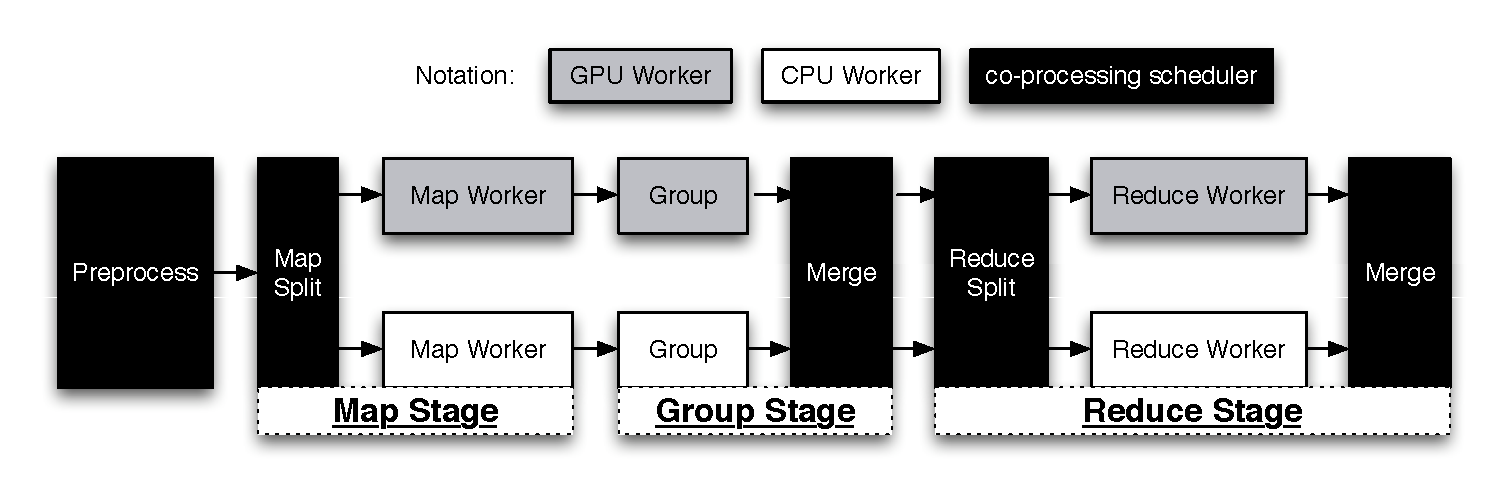
\includegraphics[width=1.00\textwidth]{figure/Mars+.eps} 
  \caption{The workflow of GPU/CPU co-processing. }\label{fig:Mars+}
\end{figure}

With the GPU/CPU co-processing module, Mars can harness the
computation power of NVIDIA GPUs, AMD GPUs, and multi-core CPUs on
the same machine, by integrating MarsCUDA, MarsBrook, and MarsCPU
modules as components.

% \chapter{Multi-machine Implementations}\label{sec-beyond}

In this chapter, we present the integration of Mars into a CPU-based distributed MapReduce system, specifically Hadoop in our implementation. 
This integration benefits from both worlds: Hadoop utilizes CPUs on multiple machines and provides fault-tolerance and other features of a distributed system; 
Mars utilizes the GPU to accelerate local computation. We denote Mars-enabled Hadoop as MarsHadoop. 

We use the {\em Hadoop Streaming}
technology~\footnote{http://hadoop.apache.org/common/docs/r0.15.2/streaming.html}
to integrate Mars into Hadoop. {\em Hadoop Streaming} enables the
developers to use their own custom Map or Reduce implementation in
Hadoop. In our implementation, we use the Mars executable to read
the input from {\em stdin} and to emit the output to {\em stdout}.
Thus, the Map and the Reduce tasks can be performed on the GPU, and
other tasks such as task scheduling and failure handling are
performed by Hadoop. Finally, since current GPUs do not support
multi-tasking, we configure MarsHadoop to run GPU-based tasks sequentially on one GPU. 


Figure \ref{fig:hadoop} illustrates the workflow of MarsHadoop. 
A Map Worker/Reduce Worker in MarsHadoop is the same as a Map Worker/Reduce Worker shown in Figure \ref{fig:Mars+}; 
in other words, it can be from MarsCUDA, MarsBrook, or MarsCPU, depending on the underlying processor. 
In the configuration of Figure \ref{fig:hadoop}, Node 1 simultaneously runs two Map Workers, on a GPU and a CPU respectively. 

\begin{figure}[ht]
  \centering
  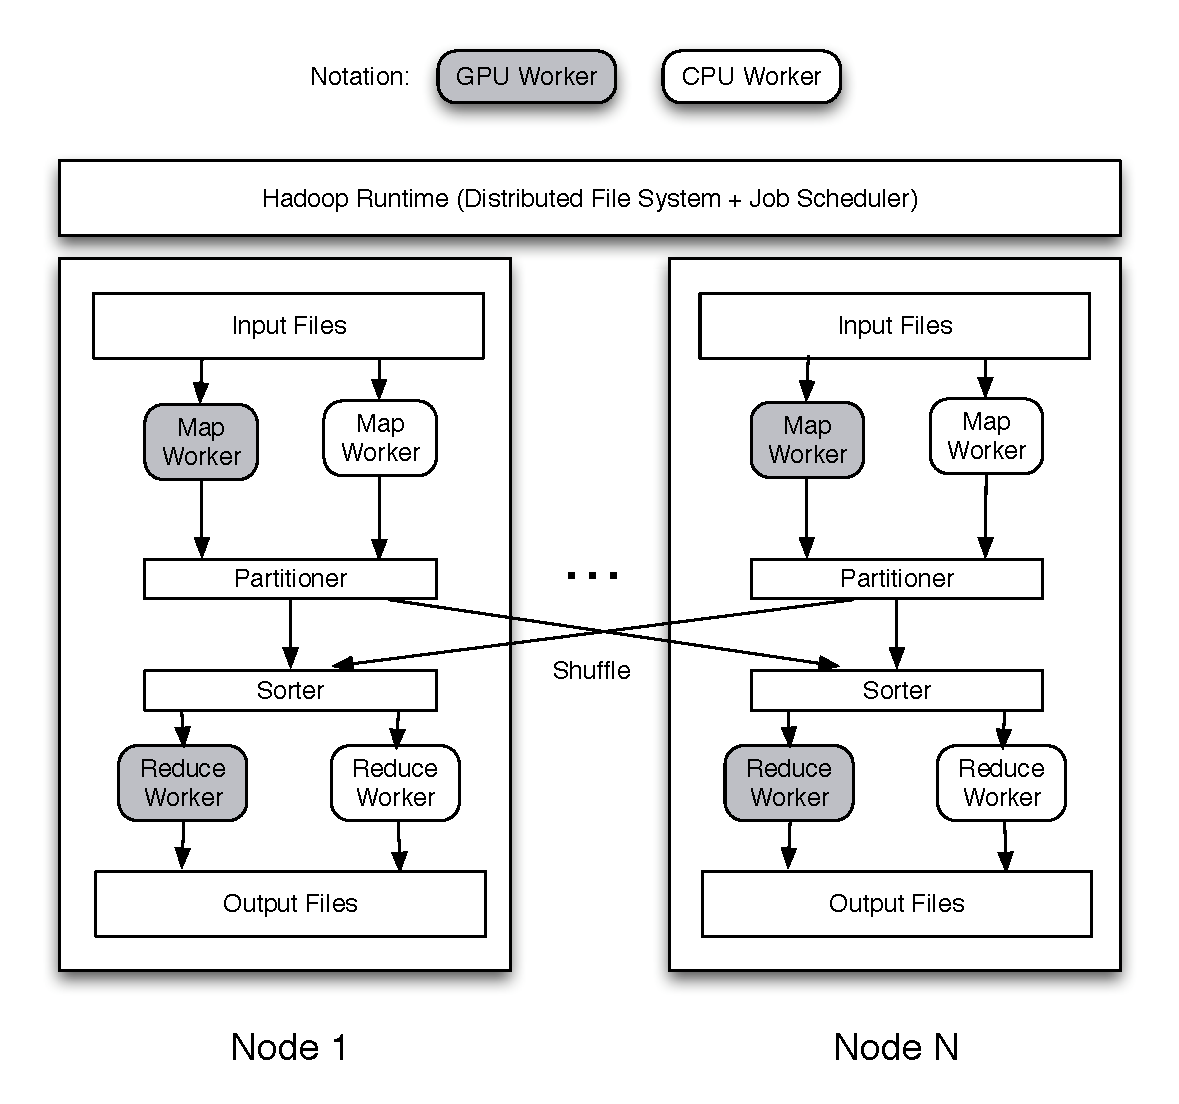
\includegraphics[width=0.70\textwidth]{figure/hadoop.eps} 
  \caption{MarsHadoop. Some Map and Reduce tasks are performed on the
  GPU, and others are on the CPU. }\label{fig:hadoop}
\end{figure}

% \chapter{Experimental Evaluation}\label{sec-eval}
In this chapter, we evaluate Mars on a single machine using a micro-benchmark of six applications in comparison with their CPU-based counterparts and native GPU-based implementations.
\red{We also evaluate the performance of MarsHadoop on two connected machines.}


\section{Experimental Setup}
Our experiments were performed on three PCs, A, B and
 C. Table \ref{tb:machines} shows their hardware configuration.
Both PCs A and B run 32-bit CentOS 5.1 Linux with kernel
2.6.18, NVIDIA CUDA 2.2, and the GPU driver 185.18.14. PC C runs
32-bit Windows XP Pro SP3, with Brook+ 1.01.0 beta, and the GPU
driver 8.561. All hard drives on these PCs are SATA magnetic hard
disks with 7200 rpm. On all PCs, the main memory and the device
memory are connected by PCI-E bus with a theoretical bandwidth of 4
GB/sec.

\doublerulesep 0.1pt
\begin{table}[htb]
  \centering
 \linespread{1.7}{ {\footnotesize
  \caption{Machine configurations}\label{tb:machines}
\vspace{2em}
  \begin{tabular}{p{4.5cm}p{3.5cm}p{3.5cm}p{3.5cm}}
  \hline
\noalign{\smallskip}
    \textbf{Machine} & \textbf{PC A}&\textbf{PC B}&\textbf{PC C}\\
\noalign{\smallskip}
  \hline
    GPU&NVIDIA GTX280& NVIDIA 8800GTX & ATI Radeon HD 3870\\
    \# GPU core & 240 & 128 & 320 \\
    GPU Core Clock (MHz)&602&575&775 \\
    GPU Memory Clock (MHz)&1107&900&2250 \\
    GPU Memory Bandwidth (GB/s)& 141.7& 86.4 &72.0\\
    GPU Memory Capacity (MB)& 1024 & 768 & 512\\
    CPU&Intel Core2 Quad Q6600 & Intel Core2 Quad Q6600 & Intel Pentium 4 540 \\
    CPU Clock (MHz)&2400&2400&3200 \\
    \# CPU core& 4 & 4 & 2\\
    CPU Memory Capacity (MB)& 2048 & 2048 & 1024\\
   \hline
 \hline
\noalign{\smallskip}
  \end{tabular}
  }}
\end{table}



\section{Micro-benchmark}

We have implemented the following six real-world applications for
evaluating the MapReduce framework.

{\bf String Match (SM):} Each Map task searches a portion of the
input file to check whether the target string is in the portion.
Neither the {\em Group} nor the {\em Reduce} stage is needed.
%The three data sets include 5 million, 10 million, and 15 million text lines to match respectively.

{\bf Matrix Multiplication (MM):} Matrix multiplication is used
intensively in analyzing the relationship of two documents. Given two
matrices $M$ and $N$, each Map task computes multiplication for a
row from $M$ and a column from $N$. It outputs the pair of the row
ID and the column ID as the key and the corresponding result as the
value. Neither the {\em Group} nor the {\em Reduce} stage is needed.
%The three data sets include about 65 thousand, 262 thousand, and 1 million pairs of row and column multiplications respectively.


{\bf Black-Scholes:} Black-Scholes model~\cite{Black1973} is used for calculating the price for European options according to a partial differential equation.
For each option, a Map task computes the prices for the call and put prices of an option, and emits a structure containing the price of the option call and the price of the option put as the key, and the option id as the value. The Group stage is to rank the price of option calls. No Reduce stage is needed.


{\bf Similarity Score (SS):} It is used in web document clustering.
The characteristics of a document are represented using a feature
vector of floating point numbers. Given two document features,
$\vec{a}$ and $\vec{b}$, the similarity score between these two
documents is defined to be $\frac{\vec{a}\cdot
\vec{b}}{|\vec{a}|\cdot |\vec{b}|}$. SS computes the pair-wise
similarity score for a set of documents. Each Map task computes the
similarity score for two documents. It outputs the intermediate pair
with the score as the key and the pair of the two document IDs as the
value. The {\em Group} stage is required to rank the pair-wise similarity
scores and no {\em Reduce} stage is required. %The three data sets include
%about 130 thousand, 262 thousand, and 1 million pairs of document
%features for calculation respectively.

\red{
{\bf Principal component analysis (PCA):} This application computes the mean vector and the covariance matrix of a set of points in the first two steps in PCA.
The input data is stored in a matrix.
The whole process contains two MapReduce invocations in a chain.
The first MapReduce procedure is to find the mean for each row in the matrix, and the second is to calculate the covariance matrix.
Neither Group nor Reduce stage is needed in the first MapReduce invocation. A Map task computes the mean for a row. In the second invocation, each Map task is to calculate the covariance of two rows.
The Group stage is required to sort the row-pairs by row IDs.
No Reduce phase is needed.
}


{\bf Monte Carlo (MC):} Monte Carlo~\cite{Boyle1977} is used to compute option pricing in financial engineering.
The Monte Carlo numeric integration is to mathematically estimate the expectation of the price of option call.
Each Map task is to compute the expected value of a random sample for an option, and to emit the option ID as the key, while the expected value of the random sample as the value.
The Group stage and the Reduce stage are required to calculate the mean of all the samples for each option.
In this application, all the options have the same number of samples, and the intermediate results are ordered by option ID already. Mars does not need to perform sorting in the Group stage.

The above applications are commonly used in benchmarking MapReduce implementations in the previous studies~\cite{Chu2006, Ranger2007}. SM, MM and PCA are adopted from Phoenix suite \cite{Ranger2007},  SS is a common component in web applications,
while BS and MC are prevalent in financial engineering, and are adopted from CUDA SDK.
In particular, the workflow of these applications differ: SM and
MM only have the {\em Map} stage, BS, SS and PCA have {\em Map} and {\em
Group} stages, and MC has all the three stages. PCA has a chain of multiple MapReduce procedures, whereas other applications have
only one MapReduce invocation.

Within a single machine, we used three data sets
for each application (S, M and L) to evaluate the scalability of the
MapReduce framework.
The input for SM is textual data, and is adopted from Phoenix~\cite{Ranger2007};
The input for all the other applications contains randomly generated real numbers, ranging from zero to one.
All these input data are stored as files in the hard disk.
We summarize the size of input data for each application in Table \ref{tab:app}.

\doublerulesep 0.1pt
\begin{table}[htb]
  \centering
 \linespread{1.7}{ {\footnotesize
  \caption{The input data sizes of the micro-benchmark}\label{tab:app}
\vspace{2em}
  \begin{tabular}{cp{3.0cm}p{3.0cm}p{3.0cm}}
  \hline
\noalign{\smallskip}
  \textbf{Applications} &  \textbf{Small} & \textbf{Medium} & \textbf{Large}\\
\noalign{\smallskip}
  \hline
  String Match  & size: 55MB & size: 105MB  & size: 160MB  \\
  Matrix Multiplication  & 256x256  &  512x512  &  1024x1024  \\
  Black-Scholes  & \# option: 1,000,000  & \# option: 3,000,000  & \# option: 5,000,000  \\
  Similarity Score  & \# feature: 128, \# documents: 512  & \# feature: 128, \# documents: 1024  & \# feature: 128, \# documents: 2048  \\
  PCA  & 1000x256  & 2000x256 &  4000x256  \\
  Monte Carlo & \# option: 500, \# samples per option: 500  &  \# option: 500, \# samples per option: 2500  &  \# option: 500, \# samples per option: 5000 \\
 \hline
\noalign{\smallskip}
  \end{tabular}
  }}
\end{table}


%With the micro benchmarks, we have compared the performance and programmability of the MapReduce frameworks between the CPU and the GPU. The third party MapReduce on the CPU is the latest release of Phoenix in version 2.0.0.  As for native implementation, we have implemented the applications directly on CUDA and pthreads.  

{\bf Metrics.} The wall time is the major metric for the
performance evaluation. \red{We measure the elapsed time of each
application from reading data from the disk till generating results
in the main memory.} We ran each experiment five times and report the
average value. The variation of elapsed time between runs is negligible.
\red{The performance speedup on A over B is defined as the running time of B divided by the running time of A.
The performance slowdown on A over B is defined as the running time of A divided by the running time of B.}

We use the number of code lines written by the user as the metric on
comparing the programmability of different MapReduce implementations
as well as the native implementation with CUDA and Brook+. Note that we exclude comments and empty lines from the code size counting.

\section{Results on a Single Machine}
On a single machine, we have compared the performance and
programmability of the MapReduce frameworks between the CPU and the
GPU. \red{We have implemented the six applications on MarsCUDA, MarsCPU, and the latest release of Phoenix in version 2.0.0.}
We have also implemented the applications directly on CUDA and pthreads respectively,
including thread configuration, data distribution, task execution,  buffer management, and various memory optimizations.

We present the results on the NVIDIA GPU in detail, and briefly
present the results on the AMD GPU, mainly demonstrating the
feasibility.
\\\\
{\em 1. Results on MarsCUDA and MarsCPU}

{\bf Programmability.} Table \ref{tab:codesize} shows the comparison
of user code size, for implementing the micro-benchmark
with MarsCUDA, MarsCPU, Phoenix, and CUDA. By design, the code sizes
with MarsCUDA are the same as those with MarsCPU. In general, the
applications with MarsCPU have a smaller code size to those with
Phoenix. Phoenix needs additional code to tune the runtime performance, for example, to setup cache sizes and data chunk size, and to specify the partition and locator functions that Mars does not require. 
If the {\em Group} stage is required, applications like
SS with MarsCUDA have a much smaller code size than that
is manually written using CUDA, due to an optimized but lengthy
group function on CUDA. \red{The user code size of MarsCUDA is up to 7 times smaller than that of the native implementation with CUDA.} 
For Matrix Multiplication, CUDA have a smaller code size, because MarsCUDA requires additional code to prepare the input key/value pairs, while the native CUDA implementation does not. 

\doublerulesep 0.1pt
\begin{table}[htb]
  \centering
 \linespread{1.7}{ {\footnotesize
  \caption{Comparison of application code size on MarsCPU, MarsCUDA, Phoenix, and  CUDA.}\label{tab:codesize}
\vspace{2em}
  \begin{tabular}{cccc}
  \hline
\noalign{\smallskip}
  \textbf{Applications} & \textbf{Phoenix} & \textbf{MarsCUDA/MarsCPU} & \textbf{CUDA} \\
\noalign{\smallskip}
  \hline
    String Match & 206 &  147 & 157 \\
  Matrix Multiplication & 178 & 72 & 68\\
  Black-Scholes & 199 & 147 & 721 \\
  Similarity Score & 125 & 82 & 615 \\
  Principal component analysis & 297 &  168 & 583 \\
  Monte Carlo & 251 &  203& 359 \\
  \hline
  \end{tabular}
  }}
\end{table}

\red{
{\bf Overall performance on MapReduce.}  We conducted the performance evaluation of MarsCUDA and MarsCPU on PC A by comparing with Phoenix. Figure~\ref{fig:overall} shows the overall performance comparison. Both MarsCUDA and MarsCPU outperform Phoenix for the
six applications, due to the general lock-free design of Mars.
}

\red{
The overall
performance of MarsCPU is generally better than
that of Phoenix, achieving a speedup of up to 25.9x. Applications written using Phoenix always have a {\em Reduce} stage, whereas using ours they may not have.
Phoenix maintains a global 2D array of pointers to keys array. Each keys array is in essence a contiguous buffer as a bucket for hashing, and is sorted by insertion sort when a new key arrives.
Such design incurs two serious performance bottlenecks. First, lock-based synchronization is needed.
Second, lots of memory buffer movements (calling {\em memmove()}) are required for insertion sort in the static array.
In contrast, the design of Mars is lock-free and each Map task or Reduce task has deterministic output buffer sizes and writing positions,
so neither lock nor memory management overhead would be introduced.
In particular, BS and SS that require to rank distinct real numbers are over 10x slower on Phoenix than on MarsCPU.
That is because Phoenix has to deploy millions of identity reduce tasks for these two applications. Our profiling results obtained from Intel VTune show that over 99\% of the total execution time of BS and SS on Phoenix is contributed to the {\em memmove()} operations in the Reduce stage.
}

\begin{figure*}[ht]
\centerline{ \subfigure[Performance speedup on MarsCPU over Phoenix]{
  \includegraphics[width=0.5\textwidth]{figure/MarsCPU_Phoenix.eps}
\label{fig:marscpu_phoenix}}
\hfill
\subfigure[Performance speedup on MarsCUDA over MarsCPU (The entire MapReduce)]{
  \includegraphics[width=0.5\textwidth]{figure/MarsGPU_MarsCPU.eps}
\label{fig:marsgpu_marscpu}}
} 

\centerline{ 
\subfigure[Performance speedup on MarsCUDA over MarsCPU (On large dataset, Map \& Reduce stages only)]{
  \includegraphics[width=0.5\textwidth]{figure/kernel.eps}
\label{fig:kernel}}
}
\caption{Performance evaluation for MarsCPU and MarsCUDA on the micro-benchmark} \label{fig:overall}
\end{figure*}

\red{
As shown in \ref{fig:kernel}, MarsCUDA utilizes the GPU hardware to accelerate the Map and Reduce stages for the 6 applications, and outperforms MarsCPU in the two stages by 21x on average, and up to 40.9x.
Please note that, this speedup is obtained without specific performance tuning on the GPU code, e.g., exploiting local memory.
When it turns to the overall performance, MarsCUDA has a 10x speedup over MarsCPU for MM,  and 6x for MC, but not so impressive speedup for the other applications (Figure \ref{fig:marsgpu_marscpu}).
}

In order to figure out the source of slowdown in overall speedup, we further investigate the time breakdown of each application on the large data set for both MarsCUDA and MarsCPU. We divide the total execution time into four components,
including the time for 1) preprocessing input data (``Preprocess"), including input file I/O, generating key/value pairs, and transfering data from main memory to device memory, 2) the
{\em Map} stage (``Map"), 3) the {\em Group} stage (``Group"), and 4) the {\em
Reduce} stage (``Reduce"). 
MarsCUDA generally has a larger portion of preprocess time, involving key-val pair preparation and PCI-E I/O. In addition, the GPU-based Group stage has limited speedup over the CPU-based. We use Amdahl's law to explain this speedup involving parallel and sequential executions. Take SM for example. Although the GPU accelerates the Map phase by 20 times, the Map only takes up some 25\% in MarsCPU. According to Amdahl's law, the theoretical speedup of MarsCUDA over MarsCPU is at most 1.3. Our measurement is close to this theoretical speedup.
The preprocess is possible to be parallelized on the multi-core CPU for MarsCUDA runtime. 
However, we leave the parallelization decision to programmers, for the consideration that the runtime system can support more general purpose applications. 

\begin{figure}[h]
\centerline{ \subfigure[Time breakdown of
MarsCUDA]{\includegraphics[width=0.50\linewidth]{figure/MarsGPU_Timebreakdown.eps}
\label{fig:timebreakdowngpu}} \hfill \subfigure[Time breakdown of
MarsCPU]{\includegraphics[width=0.50\linewidth]{figure/MarsCPU_Timebreakdown.eps}
\label{fig:timebreakdowncpu}} } \caption{Time breakdown of MarsCUDA
and MarsCPU on the micro-benchmark} \label{fig:timebreakdown}
\end{figure}

{\bf Scaling.} We used the clock rate scaling tool
NVClock~\footnote{http://www.linuxhardware.org/nvclock/} to vary the
NVIDIA GPU's core clock rate and memory clock rate, in order to
evaluate the impact of hardware capability on MarsCUDA. Figures~\ref{fig:corerate} and~\ref{fig:memoryrate} show the
performance result of the six applications running on MarsCUDA with
the large data set.

In general, most applications (except for SM) on MarsCUDA are
sensitive to both core clock rate and memory clock rate.
This result indicates that MarsCUDA can scale well as the GPU evolves.
SM is not sensitive to the hardware scaling, since its GPU computation time is relatively small (as shown in Figure~\ref{fig:timebreakdowngpu}).

\begin{figure}[ht]
\centerline{ \subfigure[Baseline: Running at 100 MHz core clock rate. Memory clock rate: fixed to 1100 MHz. ]{\includegraphics[width=0.50\linewidth]{figure/corerate.eps}
\label{fig:corerate}} \hfill \subfigure[Baseline: Running at 200 MHz memory clock rate. Core clock rate: fixed to 600 MHz. ]{\includegraphics[width=0.50\linewidth]{figure/memrate.eps}
\label{fig:memoryrate}} } \caption{Varying clock rates on GTX 280.} \label{fig:freq}
\end{figure}

{\bf Comparison with native implementation.}
Figure \ref{fig:marsgpu_cuda} shows the performance slowdown of the six applications on MarsCUDA over the native implementation, with large dataset.
Overall, the implementation of applications based on MarsCUDA has roughly the same performance as on CUDA.
However, MM and MC perform much poorer on MarsCUDA, mainly due to two reasons.
One reason is rooted at the potential deficiency of MapReduce compared with a native implementation, as a previous study has already demonstrated~\cite{Ranger2007}. The other reason is that MarsCUDA does not automatically exploit the local memory to improve the temporal locality due to the lack of knowledge about specific applications.
Similarly, Figure \ref{fig:marscpu_pthread} illustrates that applications on MarsCPU has roughly the same performance as on pthreads.

{\bf Comparison with other GPU implementations.}
There are two GPU-based MapReduce implementations in parallel to our work~\cite{Catanzaro2008,Linderman2008}, while the source code is not available in public. 
Therefore, we are not able to conduct empirical performance study by comparing with these two implementations. 
The peak speedup on the NVIDIA 8800 GTX GPU over on the CPU, reported by Catanzaro~\cite{Catanzaro2008}, is better than ours (150x vs 72x). However, their MapReduce runtime implementation is highly specialized for the machine learning workloads, and they compared with the sequential CPU code, while Mars is for general purpose applications, and we compared with parallel code. 
The Merge framework~\cite{Linderman2008} reports a peak speedup of about 23x on the Intel X3000 GPU over on the CPU, while their MapReduce design is targeted on Intel's GPUs, and Mars is a general design for different many-core processors. 

\begin{figure}[ht]
\centerline{ \subfigure[MarsCUDA over CUDA.]{\includegraphics[width=0.5\linewidth]{figure/MarsGPU_CUDA.eps}
\label{fig:marsgpu_cuda}} \hfill \subfigure[MarsCPU over pthreads.]{\includegraphics[width=0.5\linewidth]{figure/MarsCPU_pthread.eps}
\label{fig:marscpu_pthread}}
} 
\centerline{ 
\subfigure[MarsBrook over Brook+.]{\includegraphics[width=0.5\linewidth]{figure/MarsBrook_brook.eps}
\label{fig:marsbrook_brook}} 
}\caption{The performance slowdown of Mars over native implementations.}

\label{fig:slowdown}
\end{figure}

{\em 2. Results on MarsBrook}

Due to the limitation of Brook+, we have developed only two
numerical applications (i.e., MM and SS) on MarsBrook. Table
\ref{tab:brookcodesize} shows the code size of applications written
in MarsBrook compared with the native implementation in Brook+. The
result is consistent with the comparison between MarsCUDA and the
native CUDA implementation. For example, the native implementation
of SS has a much larger code size than that on MarsBrook,
since SS requires a {\em Group} stage.

\doublerulesep 0.1pt
\begin{table}[htb]
  \centering
 \linespread{1.7}{ {\footnotesize
  \caption{Comparison on code sizes of MM and SS using MarsBrook and Brook+.}\label{tab:brookcodesize}
\vspace{2em}
  \begin{tabular}{ccc}
  \hline
\noalign{\smallskip}
  \textbf{Applications} & \textbf{MarsBrook} & \textbf{Brook+} \\
\noalign{\smallskip}
  \hline
  MM & 66 & 93 \\
  SS & 66 & 611  \\
  \hline
\noalign{\smallskip}
  \end{tabular}
  }}
\end{table}

Figure \ref{fig:marsbrook_brook} shows the performance slowdown of
two applications by using MarsBrook over the native implementation.
The implementation on top of MarsBrook is up to twice slower than
the native implementation, which is the price to pay for the user code size reduction.
\\\\
{\em 3. Results on GPU/CPU co-processing of Mars}

We used MarsCUDA and MarsCPU as two components in the co-processing.
Figure \ref{fig:coprocess} shows the performance speedup of the GPU/CPU co-processing module over MarsCUDA, MarsCPU, and Phoenix, on the large dataset.
Overall, co-processing utilizes the computation power of both the CPU and the GPU, and yields a considerable performance improvement over using MarsCPU or Phoenix on a CPU.
However, the speedup of using co-processing over using standalone MarsCUDA is limited.

The workload dispatching between MarsCUDA and MarsCPU in co-processing mainly depends on the performance comparison between the CPU processing and the GPU processing.
The theoretical speedup of co-processing over MarsCUDA would be $(S + 1) / S$, where $S$ is the speedup of using MarsCUDA over using MarsCPU.
For example, if the speedup $S$ is 10, then using co-processing would only outperform using standalone MarsCUDA by a factor of $\frac{10+1}{10} = 1.1$.
Therefore, for compute-intensive applications MM, BS, SS, MC, and PCA, using co-processing cannot boost the performance considerably over using the standalone MarsCUDA.
For SM that spends most time in preprocessing, using co-processing can hardly achieve the theoretical speedup $\frac{1+1}{1} = 2$.
Nevertheless, applications using co-processing of MarsCUDA and MarsCPU still outperforms Phoenix with a speedup of 24 times on average, and 72 times at maximum.

\begin{figure}[h]
 \centering
 \includegraphics[width=0.65\textwidth]{figure/coprocess.eps}
 \caption{Performance speedup of GPU/CPU co-processing module over MarsCUDA, MarsCPU, and Phoenix.}\label{fig:coprocess}
\end{figure}


\section{Results on MarsHadoop}

We experimented MM on MarsHadoop. We configured Hadoop on
PC A and PC B: PC A as the master node, while PC A itself and PC B
as slave nodes.


Figure \ref{fig:hadoopspeedup} shows the performance speedup of
MarsHadoop over the native Hadoop implementation on MM. As the
matrix size varied, MarsHadoop is up to 2.8 times faster than the
native Hadoop implementation. We further examine the time breakdown
in the slave node, and the results are shown in Figure
\ref{fig:hadoopmmbreakdown}. As the matrix size increases, the ratio
for the computation time grows, indicating that Mars starts to help.
The disk I/O is mainly due to the extra I/O caused by Hadoop
streaming.

\begin{figure}[h]
\centerline{
\subfigure[Performance speedup on MarsHadoop over native Hadoop.]{\includegraphics[width=0.50\linewidth]{figure/speeduphadoop.eps}
\label{fig:hadoopspeedup}}
\hfill
\subfigure[Time breakdown on MarsHadoop.]{\includegraphics[width=0.5\linewidth]{figure/breakdownhadoop.eps}
\label{fig:hadoopmmbreakdown}} } \caption{Matrix Multiplication on MarsHadoop}
\end{figure}


% \chapter{Conclusion}\label{sec-conclusion}
Graphics processors have become an efficient accelerator for
high-performance computing. This thesis proposes Mars, which
harnesses the GPU computation power and high memory bandwidth to
accelerate MapReduce frameworks. Mars is applicable to run on
NVIDIA GPUs, AMD GPUs, multi-core CPUs, and Hadoop-based distributed systems. 
%and can be easily ported to other parallel systems, due to its lock-free design and simple array data structure. 
%In addition, Mars is flexible enough to support a variety of applications efficiently, because of the support of customized workflow. 
Our empirical studies show that Mars
improves the programmability of both the NVIDIA and the AMD GPUs,
and \red{the GPU-CPU co-processing of Mars on an NVIDIA GTX280 GPU and an Intel quad-core CPU outperformed Phoenix, the state-of-the-art MapReduce on the multi-core CPU with a speedup of up to 72 times and 24 times on average.} Additionally, integrating Mars into Hadoop enabled GPU acceleration for a network of PCs.

The code and documentation of Mars can be found at
http://www.cse.ust.hk/gpuqp/.



%%%%%%%%%%%%%%%%%%%%%%%%%%%%%%%%%%%%%%%%%%%%%%%%%%%%%%%%%%%%%%%%%%%%%%%%%
%                                                                       %
%      9) BIBLIOGRAPHY                                                  %
%                                                                       %
% This example uses bibtex to generate the required Bibliography. Refer %
% to the % the file ustthesis_test.bib for the entries of the           %
% Bibliography. Note that only the cited entries are printed.           %
%                                                                       %
% If BibTeX is not used to typeset the bibliography, replace the        %
% following line with the \begin{thebibliography} and \end{bibliography}%
% commands (the "thebibliography" environment) to process the           %
% Bibliography.                                                         %
%                                                                       %
%%%%%%%%%%%%%%%%%%%%%%%%%%%%%%%%%%%%%%%%%%%%%%%%%%%%%%%%%%%%%%%%%%%%%%%%%

%%%%%%%%%%%%%%%%%%%%%%%%%%%%%%%%%%%%%%%%%%%%%%%%%%%%%%%%%%%%%%%%%%%%%%%%%
%                                                                       %
% The recommended bibliography style is the IEEE bibliography style.    %
% "ustbib" defines the IEEE bibliography standard with the added        %
% ability of sorting the items by name of author.                       %
%                                                                       %
% If you are not using BibTeX to process your Bibliography, comment out %
% the following line.                                                   %
%                                                                       %
%%%%%%%%%%%%%%%%%%%%%%%%%%%%%%%%%%%%%%%%%%%%%%%%%%%%%%%%%%%%%%%%%%%%%%%%%

\bibliographystyle{plain}

\bibliography{ref}
% Please run "bibtex ustthesis_test" before the bibliography can be
% included.

%%%%%%%%%%%%%%%%%%%%%%%%%%%%%%%%%%%%%%%%%%%%%%%%%%%%%%%%%%%%%%%%%%%%%%%%%
%                                                                       %
%     10) APPENDIX (If Any)                                              %
%                                                                       %
% \appendix command marks the beginning of the APPENDIX part of the     %
% Thesis. The usual \chapter command is used for the different chapters %
% of the Appendix.                                                      %
%                                                                       %
%%%%%%%%%%%%%%%%%%%%%%%%%%%%%%%%%%%%%%%%%%%%%%%%%%%%%%%%%%%%%%%%%%%%%%%%%


%%%%%%%%%%%%%%%%%%%%%%%%%%%%%%%%%%%%%%%%%%%%%%%%%%%%%%%%%%%%%%%%%%%%%%%%%
%                                                                       %
%     11) BIOGRAPHY (Optional)                                          %
%                                                                       %
% \biography and \endbiography are used to define the optional          %
% Biography of the author of the Thesis.                                %
%                                                                       %
%%%%%%%%%%%%%%%%%%%%%%%%%%%%%%%%%%%%%%%%%%%%%%%%%%%%%%%%%%%%%%%%%%%%%%%%%

% \biography
% The biography of the student is ALSO optional.
% \endbiography

\end{document}
